% =====================================================================
% The per-dataset results, copied from the supplementary material of
% the paper.
%
% Organised as one subsection per dataset, each opening with its own
% prose and followed by its own tables, so that a table is never far
% from the text that refers to it. \FloatBarrier closes every
% subsection, which stops a float drifting into the next one.
%
% The tables themselves are generated by run_relaxation_sweep.py in the
% repository of the paper: regenerate between the AUTO markers, do not
% edit the rows by hand.
% =====================================================================

\subsection{Overview of the Results}
\label{sec:evaluation-results-overview}

We next show the execution time and the analysis tightness of all perturbations.
Figures~\ref{fig:n2-time-app} and~\ref{fig:n2-time-app-2} show the execution time as bars and the
analysis tightness as a black line, a box per perturbation and group of networks. The results show that
\tool is faster than \baseline on most perturbations, and transfer mode provides additional speedup.
Figures~\ref{fig:n2-bounddiff-app},~\ref{fig:n2-bounddiff-app-2}
and~\ref{fig:n2-bounddiff-app-3} show the analysis tightness on the instances where all
three verifiers reach the timeout. The results show that
\tool achieves tighter bounds than \baseline on these instances as well. Transfer mode improves them further on CIFAR-10 \emph{conv4}, where the average $\delta_u{-}\delta_l$ ratio grows from $3\times$ to $7.5\times$. On the other networks the two modes are close: $27.4\times$ and $27.5\times$ on MNIST, $1.7\times$ in both modes on Fashion-MNIST, and $65.8\times$ and $65.6\times$ on HAR.
The individual experiments behind these figures are in the detailed tables:
Tables~\ref{tab:mnist-timeout} and~\ref{tab:mnist-solved} for MNIST,
Tables~\ref{tab:fashion-timeout} and~\ref{tab:fashion-solved} for Fashion-MNIST,
Tables~\ref{tab:cifar-timeout} and~\ref{tab:cifar-solved} for CIFAR-10,
and Table~\ref{tab:har-timeout} for HAR.

% BEGIN AUTO: aaai_n2_time_appendix
% Every box is one axis, drawn by tools/build_time_figures.py from the
% numbers of the solve-time pdfs of the paper. A perturbation that runs
% to more class pairs than one text block holds is split over several
% boxes, so that every box keeps the same bar width; the boxes are then
% stacked here, so that one legend and one caption serve them all.

\begin{figure}[p]
\centering

\includegraphics[trim=117 102.604 118 0,clip]{graphics/n2_time_app}

\vspace{8pt}

% ===================================================================
% Written by tools/build_time_figures.py -- do not edit by hand.
% One axis for every experiment of this perturbation, rebuilt from
% the numbers of the pdfs the paper generates, in their colours.
% ===================================================================
\definecolor{blendtr}{rgb}{0.083,0.301,0.083}
\definecolor{blendpl}{rgb}{0.652,0.844,0.652}
\definecolor{vhagarcol}{rgb}{0.753,0.314,0.302}
\begin{tikzpicture}[x=1pt,y=1pt,font=\fontsize{9}{10.5}\selectfont]
  \fill[black!3] (0,0) rectangle (321.00,62.50);
  \fill[blendtr] (0.00,0) rectangle (5.50,18.48);
  \draw[black!60,line width=0.2pt] (0.00,0) rectangle (5.50,18.48);
  \fill[blendpl] (5.50,0) rectangle (11.00,29.95);
  \fill[pattern=north east lines,pattern color=blendtr] (5.50,0) rectangle (11.00,29.95);
  \draw[black!60,line width=0.2pt] (5.50,0) rectangle (11.00,29.95);
  \fill[vhagarcol] (11.00,0) rectangle (16.50,48.05);
  \draw[black!60,line width=0.2pt] (11.00,0) rectangle (16.50,48.05);
  \draw[black,line width=0.3pt] (2.75,0.31) -- (8.25,0.31) -- (13.75,7.26);
  \fill[black] (2.75,0.31) circle (0.75pt);
  \fill[black] (8.25,0.31) circle (0.75pt);
  \fill[black] (13.75,7.26) circle (0.75pt);
  \fill[blendtr] (30.05,0) rectangle (35.55,44.58);
  \draw[black!60,line width=0.2pt] (30.05,0) rectangle (35.55,44.58);
  \fill[blendpl] (35.55,0) rectangle (41.05,38.76);
  \fill[pattern=north east lines,pattern color=blendtr] (35.55,0) rectangle (41.05,38.76);
  \draw[black!60,line width=0.2pt] (35.55,0) rectangle (41.05,38.76);
  \fill[vhagarcol] (41.05,0) rectangle (46.55,48.05);
  \draw[black!60,line width=0.2pt] (41.05,0) rectangle (46.55,48.05);
  \draw[black,line width=0.3pt] (32.80,0.34) -- (38.30,0.34) -- (43.80,7.96);
  \fill[black] (32.80,0.34) circle (0.75pt);
  \fill[black] (38.30,0.34) circle (0.75pt);
  \fill[black] (43.80,7.96) circle (0.75pt);
  \fill[blendtr] (51.03,0) rectangle (56.53,5.59);
  \draw[black!60,line width=0.2pt] (51.03,0) rectangle (56.53,5.59);
  \fill[blendpl] (56.53,0) rectangle (62.03,5.21);
  \fill[pattern=north east lines,pattern color=blendtr] (56.53,0) rectangle (62.03,5.21);
  \draw[black!60,line width=0.2pt] (56.53,0) rectangle (62.03,5.21);
  \fill[vhagarcol] (62.03,0) rectangle (67.53,48.05);
  \draw[black!60,line width=0.2pt] (62.03,0) rectangle (67.53,48.05);
  \draw[black,line width=0.3pt] (53.78,0.27) -- (59.28,0.27) -- (64.78,9.46);
  \fill[black] (53.78,0.27) circle (0.75pt);
  \fill[black] (59.28,0.27) circle (0.75pt);
  \fill[black] (64.78,9.46) circle (0.75pt);
  \fill[blendtr] (73.53,0) rectangle (79.03,47.25);
  \draw[black!60,line width=0.2pt] (73.53,0) rectangle (79.03,47.25);
  \fill[blendpl] (79.03,0) rectangle (84.53,27.42);
  \fill[pattern=north east lines,pattern color=blendtr] (79.03,0) rectangle (84.53,27.42);
  \draw[black!60,line width=0.2pt] (79.03,0) rectangle (84.53,27.42);
  \fill[vhagarcol] (84.53,0) rectangle (90.03,48.05);
  \draw[black!60,line width=0.2pt] (84.53,0) rectangle (90.03,48.05);
  \draw[black,line width=0.3pt] (76.28,0.27) -- (81.78,0.27) -- (87.28,11.01);
  \fill[black] (76.28,0.27) circle (0.75pt);
  \fill[black] (81.78,0.27) circle (0.75pt);
  \fill[black] (87.28,11.01) circle (0.75pt);
  \fill[blendtr] (94.51,0) rectangle (100.01,2.76);
  \draw[black!60,line width=0.2pt] (94.51,0) rectangle (100.01,2.76);
  \fill[blendpl] (100.01,0) rectangle (105.51,2.51);
  \fill[pattern=north east lines,pattern color=blendtr] (100.01,0) rectangle (105.51,2.51);
  \draw[black!60,line width=0.2pt] (100.01,0) rectangle (105.51,2.51);
  \fill[vhagarcol] (105.51,0) rectangle (111.01,48.05);
  \draw[black!60,line width=0.2pt] (105.51,0) rectangle (111.01,48.05);
  \draw[black,line width=0.3pt] (97.26,0.19) -- (102.76,0.19) -- (108.26,9.67);
  \fill[black] (97.26,0.19) circle (0.75pt);
  \fill[black] (102.76,0.19) circle (0.75pt);
  \fill[black] (108.26,9.67) circle (0.75pt);
  \fill[blendtr] (124.55,0) rectangle (130.05,0.24);
  \draw[black!60,line width=0.2pt] (124.55,0) rectangle (130.05,0.24);
  \fill[blendpl] (130.05,0) rectangle (135.55,3.91);
  \fill[pattern=north east lines,pattern color=blendtr] (130.05,0) rectangle (135.55,3.91);
  \draw[black!60,line width=0.2pt] (130.05,0) rectangle (135.55,3.91);
  \fill[vhagarcol] (135.55,0) rectangle (141.05,48.05);
  \draw[black!60,line width=0.2pt] (135.55,0) rectangle (141.05,48.05);
  \draw[black,line width=0.3pt] (127.30,0.12) -- (132.80,0.00) -- (138.30,30.78);
  \fill[black] (127.30,0.12) circle (0.75pt);
  \fill[black] (132.80,0.00) circle (0.75pt);
  \fill[black] (138.30,30.78) circle (0.75pt);
  \fill[blendtr] (145.53,0) rectangle (151.03,0.74);
  \draw[black!60,line width=0.2pt] (145.53,0) rectangle (151.03,0.74);
  \fill[blendpl] (151.03,0) rectangle (156.53,1.30);
  \fill[pattern=north east lines,pattern color=blendtr] (151.03,0) rectangle (156.53,1.30);
  \draw[black!60,line width=0.2pt] (151.03,0) rectangle (156.53,1.30);
  \fill[vhagarcol] (156.53,0) rectangle (162.03,48.05);
  \draw[black!60,line width=0.2pt] (156.53,0) rectangle (162.03,48.05);
  \draw[black,line width=0.3pt] (148.28,0.10) -- (153.78,0.08) -- (159.28,9.08);
  \fill[black] (148.28,0.10) circle (0.75pt);
  \fill[black] (153.78,0.08) circle (0.75pt);
  \fill[black] (159.28,9.08) circle (0.75pt);
  \fill[blendtr] (168.03,0) rectangle (173.53,0.26);
  \draw[black!60,line width=0.2pt] (168.03,0) rectangle (173.53,0.26);
  \fill[blendpl] (173.53,0) rectangle (179.03,0.16);
  \fill[pattern=north east lines,pattern color=blendtr] (173.53,0) rectangle (179.03,0.16);
  \draw[black!60,line width=0.2pt] (173.53,0) rectangle (179.03,0.16);
  \fill[vhagarcol] (179.03,0) rectangle (184.53,5.63);
  \draw[black!60,line width=0.2pt] (179.03,0) rectangle (184.53,5.63);
  \draw[black,line width=0.3pt] (170.78,0.04) -- (176.28,0.05) -- (181.78,0.03);
  \fill[black] (170.78,0.04) circle (0.75pt);
  \fill[black] (176.28,0.05) circle (0.75pt);
  \fill[black] (181.78,0.03) circle (0.75pt);
  \fill[blendtr] (189.01,0) rectangle (194.51,0.66);
  \draw[black!60,line width=0.2pt] (189.01,0) rectangle (194.51,0.66);
  \fill[blendpl] (194.51,0) rectangle (200.01,0.56);
  \fill[pattern=north east lines,pattern color=blendtr] (194.51,0) rectangle (200.01,0.56);
  \draw[black!60,line width=0.2pt] (194.51,0) rectangle (200.01,0.56);
  \fill[vhagarcol] (200.01,0) rectangle (205.51,48.05);
  \draw[black!60,line width=0.2pt] (200.01,0) rectangle (205.51,48.05);
  \draw[black,line width=0.3pt] (191.76,0.05) -- (197.26,0.00) -- (202.76,14.11);
  \fill[black] (191.76,0.05) circle (0.75pt);
  \fill[black] (197.26,0.00) circle (0.75pt);
  \fill[black] (202.76,14.11) circle (0.75pt);
  \fill[blendtr] (219.06,0) rectangle (224.56,2.57);
  \draw[black!60,line width=0.2pt] (219.06,0) rectangle (224.56,2.57);
  \fill[blendpl] (224.56,0) rectangle (230.06,48.05);
  \fill[pattern=north east lines,pattern color=blendtr] (224.56,0) rectangle (230.06,48.05);
  \draw[black!60,line width=0.2pt] (224.56,0) rectangle (230.06,48.05);
  \fill[vhagarcol] (230.06,0) rectangle (235.56,48.05);
  \draw[black!60,line width=0.2pt] (230.06,0) rectangle (235.56,48.05);
  \draw[black,line width=0.3pt] (221.81,0.03) -- (227.31,6.87) -- (232.81,0.00);
  \fill[black] (221.81,0.03) circle (0.75pt);
  \fill[black] (227.31,6.87) circle (0.75pt);
  \fill[black] (232.81,0.00) circle (0.75pt);
  \fill[blendtr] (240.04,0) rectangle (245.54,34.17);
  \draw[black!60,line width=0.2pt] (240.04,0) rectangle (245.54,34.17);
  \fill[blendpl] (245.54,0) rectangle (251.04,48.05);
  \fill[pattern=north east lines,pattern color=blendtr] (245.54,0) rectangle (251.04,48.05);
  \draw[black!60,line width=0.2pt] (245.54,0) rectangle (251.04,48.05);
  \fill[vhagarcol] (251.04,0) rectangle (256.54,48.05);
  \draw[black!60,line width=0.2pt] (251.04,0) rectangle (256.54,48.05);
  \draw[black,line width=0.3pt] (242.79,0.25) -- (248.29,11.91) -- (253.79,41.68);
  \fill[black] (242.79,0.25) circle (0.75pt);
  \fill[black] (248.29,11.91) circle (0.75pt);
  \fill[black] (253.79,41.68) circle (0.75pt);
  \fill[blendtr] (262.54,0) rectangle (268.04,4.24);
  \draw[black!60,line width=0.2pt] (262.54,0) rectangle (268.04,4.24);
  \fill[blendpl] (268.04,0) rectangle (273.54,48.05);
  \fill[pattern=north east lines,pattern color=blendtr] (268.04,0) rectangle (273.54,48.05);
  \draw[black!60,line width=0.2pt] (268.04,0) rectangle (273.54,48.05);
  \fill[vhagarcol] (273.54,0) rectangle (279.04,48.05);
  \draw[black!60,line width=0.2pt] (273.54,0) rectangle (279.04,48.05);
  \draw[black,line width=0.3pt] (265.29,0.19) -- (270.79,1.83) -- (276.29,45.91);
  \fill[black] (265.29,0.19) circle (0.75pt);
  \fill[black] (270.79,1.83) circle (0.75pt);
  \fill[black] (276.29,45.91) circle (0.75pt);
  \fill[blendtr] (283.52,0) rectangle (289.02,1.93);
  \draw[black!60,line width=0.2pt] (283.52,0) rectangle (289.02,1.93);
  \fill[blendpl] (289.02,0) rectangle (294.52,37.13);
  \fill[pattern=north east lines,pattern color=blendtr] (289.02,0) rectangle (294.52,37.13);
  \draw[black!60,line width=0.2pt] (289.02,0) rectangle (294.52,37.13);
  \fill[vhagarcol] (294.52,0) rectangle (300.02,48.05);
  \draw[black!60,line width=0.2pt] (294.52,0) rectangle (300.02,48.05);
  \draw[black,line width=0.3pt] (286.27,0.06) -- (291.77,0.18) -- (297.27,41.27);
  \fill[black] (286.27,0.06) circle (0.75pt);
  \fill[black] (291.77,0.18) circle (0.75pt);
  \fill[black] (297.27,41.27) circle (0.75pt);
  \fill[blendtr] (304.50,0) rectangle (310.00,2.66);
  \draw[black!60,line width=0.2pt] (304.50,0) rectangle (310.00,2.66);
  \fill[blendpl] (310.00,0) rectangle (315.50,48.05);
  \fill[pattern=north east lines,pattern color=blendtr] (310.00,0) rectangle (315.50,48.05);
  \draw[black!60,line width=0.2pt] (310.00,0) rectangle (315.50,48.05);
  \fill[vhagarcol] (315.50,0) rectangle (321.00,48.05);
  \draw[black!60,line width=0.2pt] (315.50,0) rectangle (321.00,48.05);
  \draw[black,line width=0.3pt] (307.25,0.08) -- (312.75,1.82) -- (318.25,34.75);
  \fill[black] (307.25,0.08) circle (0.75pt);
  \fill[black] (312.75,1.82) circle (0.75pt);
  \fill[black] (318.25,34.75) circle (0.75pt);
  \draw[black!60,line width=0.3pt] (0,0) rectangle (321.00,62.50);
  \draw[black,dashed,line width=0.3pt] (0,48.05) -- (321.00,48.05);
  \draw[black!60,line width=0.3pt] (0,0.00) -- (-2,0.00) node[left,inner sep=1pt,font=\fontsize{10.95}{13}\selectfont] {0};
  \draw[black!60,line width=0.3pt] (0,26.69) -- (-2,26.69) node[left,inner sep=1pt,font=\fontsize{10.95}{13}\selectfont] {100};
  \draw[black!60,line width=0.3pt] (0,53.39) -- (-2,53.39) node[left,inner sep=1pt,font=\fontsize{10.95}{13}\selectfont] {200};
  \node[rotate=90,anchor=south,font=\fontsize{10.95}{13}\selectfont] at (-26.0,31.25) {time (minutes)};
  \draw[black!60,line width=0.3pt] (321.00,0.00) -- (323.00,0.00) node[right,inner sep=1pt,font=\fontsize{10.95}{13}\selectfont] {0};
  \draw[black!60,line width=0.3pt] (321.00,24.02) -- (323.00,24.02) node[right,inner sep=1pt,font=\fontsize{10.95}{13}\selectfont] {50};
  \draw[black!60,line width=0.3pt] (321.00,48.05) -- (323.00,48.05) node[right,inner sep=1pt,font=\fontsize{10.95}{13}\selectfont] {100};
  \node[rotate=90,anchor=north,font=\fontsize{10.95}{13}\selectfont] at (347.00,31.25) {$\delta_u-\delta_l$ (\%$\delta_{\max}$)};
  \node[above,inner sep=1.5pt,font=\fontsize{10.95}{13}\selectfont] at (160.50,75.50) {patch};
  \node[above,inner sep=1.5pt,font=\fontsize{9}{10.5}\selectfont] at (160.50,64.00) {(1,14,14,3)};
  \draw[black,line width=0.25pt] (0.00,-1.5) -- (0.00,-3) -- (16.50,-3) -- (16.50,-1.5);
  \node[below,inner sep=1.5pt,font=\fontsize{9}{10.5}\selectfont] at (8.25,-3) {$c_s{=}0$};
  \draw[black,line width=0.25pt] (30.05,-1.5) -- (30.05,-3) -- (67.53,-3) -- (67.53,-1.5);
  \node[below,inner sep=1.5pt,font=\fontsize{9}{10.5}\selectfont] at (48.79,-3) {$c_s{=}0$};
  \draw[black,line width=0.25pt] (73.53,-1.5) -- (73.53,-3) -- (111.01,-3) -- (111.01,-1.5);
  \node[below,inner sep=1.5pt,font=\fontsize{9}{10.5}\selectfont] at (92.27,-3) {$c_s{=}2$};
  \draw[black,line width=0.25pt] (124.55,-1.5) -- (124.55,-3) -- (162.03,-3) -- (162.03,-1.5);
  \node[below,inner sep=1.5pt,font=\fontsize{9}{10.5}\selectfont] at (143.29,-3) {$c_s{=}0$};
  \draw[black,line width=0.25pt] (168.03,-1.5) -- (168.03,-3) -- (205.51,-3) -- (205.51,-1.5);
  \node[below,inner sep=1.5pt,font=\fontsize{9}{10.5}\selectfont] at (186.77,-3) {$c_s{=}2$};
  \draw[black,line width=0.25pt] (219.06,-1.5) -- (219.06,-3) -- (256.54,-3) -- (256.54,-1.5);
  \node[below,inner sep=1.5pt,font=\fontsize{9}{10.5}\selectfont] at (237.80,-3) {$c_s{=}0$};
  \draw[black,line width=0.25pt] (262.54,-1.5) -- (262.54,-3) -- (321.00,-3) -- (321.00,-1.5);
  \node[below,inner sep=1.5pt,font=\fontsize{9}{10.5}\selectfont] at (291.77,-3) {$c_s{=}2$};
  \node[below,align=center,inner sep=1pt,font=\fontsize{9}{10.5}\selectfont\bfseries] at (8.25,-15.00) {3$\times$50\\MNIST};
  \node[below,align=center,inner sep=1pt,font=\fontsize{9}{10.5}\selectfont\bfseries] at (70.53,-15.00) {3$\times$50\\FMNIST};
  \node[below,align=center,inner sep=1pt,font=\fontsize{9}{10.5}\selectfont\bfseries] at (165.03,-15.00) {\emph{conv1}\\MNIST};
  \node[below,align=center,inner sep=1pt,font=\fontsize{9}{10.5}\selectfont\bfseries] at (270.03,-15.00) {\emph{conv4}\\CIFAR-10};
\end{tikzpicture}


\vspace{8pt}

% ===================================================================
% Written by tools/build_time_figures.py -- do not edit by hand.
% One axis for every experiment of this perturbation, rebuilt from
% the numbers of the pdfs the paper generates, in their colours.
% ===================================================================
\definecolor{blendtr}{rgb}{0.083,0.301,0.083}
\definecolor{blendpl}{rgb}{0.652,0.844,0.652}
\definecolor{vhagarcol}{rgb}{0.753,0.314,0.302}
\begin{tikzpicture}[x=1pt,y=1pt,font=\fontsize{9}{10.5}\selectfont]
  \fill[black!3] (0,0) rectangle (321.00,62.50);
  \fill[blendtr] (0.00,0) rectangle (4.57,1.31);
  \draw[black!60,line width=0.2pt] (0.00,0) rectangle (4.57,1.31);
  \fill[blendpl] (4.57,0) rectangle (9.14,1.13);
  \fill[pattern=north east lines,pattern color=blendtr] (4.57,0) rectangle (9.14,1.13);
  \draw[black!60,line width=0.2pt] (4.57,0) rectangle (9.14,1.13);
  \fill[vhagarcol] (9.14,0) rectangle (13.72,5.47);
  \draw[black!60,line width=0.2pt] (9.14,0) rectangle (13.72,5.47);
  \draw[black,line width=0.3pt] (2.29,0.42) -- (6.86,0.42) -- (11.43,0.40);
  \fill[black] (2.29,0.42) circle (0.75pt);
  \fill[black] (6.86,0.42) circle (0.75pt);
  \fill[black] (11.43,0.40) circle (0.75pt);
  \fill[blendtr] (19.72,0) rectangle (24.29,1.23);
  \draw[black!60,line width=0.2pt] (19.72,0) rectangle (24.29,1.23);
  \fill[blendpl] (24.29,0) rectangle (28.86,2.22);
  \fill[pattern=north east lines,pattern color=blendtr] (24.29,0) rectangle (28.86,2.22);
  \draw[black!60,line width=0.2pt] (24.29,0) rectangle (28.86,2.22);
  \fill[vhagarcol] (28.86,0) rectangle (33.43,19.08);
  \draw[black!60,line width=0.2pt] (28.86,0) rectangle (33.43,19.08);
  \draw[black,line width=0.3pt] (22.00,0.16) -- (26.57,0.18) -- (31.14,0.46);
  \fill[black] (22.00,0.16) circle (0.75pt);
  \fill[black] (26.57,0.18) circle (0.75pt);
  \fill[black] (31.14,0.46) circle (0.75pt);
  \fill[blendtr] (37.91,0) rectangle (42.48,0.77);
  \draw[black!60,line width=0.2pt] (37.91,0) rectangle (42.48,0.77);
  \fill[blendpl] (42.48,0) rectangle (47.05,1.59);
  \fill[pattern=north east lines,pattern color=blendtr] (42.48,0) rectangle (47.05,1.59);
  \draw[black!60,line width=0.2pt] (42.48,0) rectangle (47.05,1.59);
  \fill[vhagarcol] (47.05,0) rectangle (51.63,5.00);
  \draw[black!60,line width=0.2pt] (47.05,0) rectangle (51.63,5.00);
  \draw[black,line width=0.3pt] (40.20,0.00) -- (44.77,0.00) -- (49.34,0.47);
  \fill[black] (40.20,0.00) circle (0.75pt);
  \fill[black] (44.77,0.00) circle (0.75pt);
  \fill[black] (49.34,0.47) circle (0.75pt);
  \fill[blendtr] (56.11,0) rectangle (60.68,3.27);
  \draw[black!60,line width=0.2pt] (56.11,0) rectangle (60.68,3.27);
  \fill[blendpl] (60.68,0) rectangle (65.25,5.31);
  \fill[pattern=north east lines,pattern color=blendtr] (60.68,0) rectangle (65.25,5.31);
  \draw[black!60,line width=0.2pt] (60.68,0) rectangle (65.25,5.31);
  \fill[vhagarcol] (65.25,0) rectangle (69.82,29.87);
  \draw[black!60,line width=0.2pt] (65.25,0) rectangle (69.82,29.87);
  \draw[black,line width=0.3pt] (58.39,0.20) -- (62.96,0.27) -- (67.54,0.46);
  \fill[black] (58.39,0.20) circle (0.75pt);
  \fill[black] (62.96,0.27) circle (0.75pt);
  \fill[black] (67.54,0.46) circle (0.75pt);
  \fill[blendtr] (75.82,0) rectangle (80.39,0.70);
  \draw[black!60,line width=0.2pt] (75.82,0) rectangle (80.39,0.70);
  \fill[blendpl] (80.39,0) rectangle (84.96,0.72);
  \fill[pattern=north east lines,pattern color=blendtr] (80.39,0) rectangle (84.96,0.72);
  \draw[black!60,line width=0.2pt] (80.39,0) rectangle (84.96,0.72);
  \fill[vhagarcol] (84.96,0) rectangle (89.54,4.28);
  \draw[black!60,line width=0.2pt] (84.96,0) rectangle (89.54,4.28);
  \draw[black,line width=0.3pt] (78.11,0.46) -- (82.68,0.40) -- (87.25,0.41);
  \fill[black] (78.11,0.46) circle (0.75pt);
  \fill[black] (82.68,0.40) circle (0.75pt);
  \fill[black] (87.25,0.41) circle (0.75pt);
  \fill[blendtr] (94.02,0) rectangle (98.59,2.07);
  \draw[black!60,line width=0.2pt] (94.02,0) rectangle (98.59,2.07);
  \fill[blendpl] (98.59,0) rectangle (103.16,1.99);
  \fill[pattern=north east lines,pattern color=blendtr] (98.59,0) rectangle (103.16,1.99);
  \draw[black!60,line width=0.2pt] (98.59,0) rectangle (103.16,1.99);
  \fill[vhagarcol] (103.16,0) rectangle (107.73,20.98);
  \draw[black!60,line width=0.2pt] (103.16,0) rectangle (107.73,20.98);
  \draw[black,line width=0.3pt] (96.30,0.39) -- (100.87,0.36) -- (105.45,0.39);
  \fill[black] (96.30,0.39) circle (0.75pt);
  \fill[black] (100.87,0.36) circle (0.75pt);
  \fill[black] (105.45,0.39) circle (0.75pt);
  \fill[blendtr] (113.73,0) rectangle (118.30,5.07);
  \draw[black!60,line width=0.2pt] (113.73,0) rectangle (118.30,5.07);
  \fill[blendpl] (118.30,0) rectangle (122.88,4.32);
  \fill[pattern=north east lines,pattern color=blendtr] (118.30,0) rectangle (122.88,4.32);
  \draw[black!60,line width=0.2pt] (118.30,0) rectangle (122.88,4.32);
  \fill[vhagarcol] (122.88,0) rectangle (127.45,48.05);
  \draw[black!60,line width=0.2pt] (122.88,0) rectangle (127.45,48.05);
  \draw[black,line width=0.3pt] (116.02,0.47) -- (120.59,0.47) -- (125.16,0.79);
  \fill[black] (116.02,0.47) circle (0.75pt);
  \fill[black] (120.59,0.47) circle (0.75pt);
  \fill[black] (125.16,0.79) circle (0.75pt);
  \fill[blendtr] (131.93,0) rectangle (136.50,1.82);
  \draw[black!60,line width=0.2pt] (131.93,0) rectangle (136.50,1.82);
  \fill[blendpl] (136.50,0) rectangle (141.07,14.88);
  \fill[pattern=north east lines,pattern color=blendtr] (136.50,0) rectangle (141.07,14.88);
  \draw[black!60,line width=0.2pt] (136.50,0) rectangle (141.07,14.88);
  \fill[vhagarcol] (141.07,0) rectangle (145.64,48.05);
  \draw[black!60,line width=0.2pt] (141.07,0) rectangle (145.64,48.05);
  \draw[black,line width=0.3pt] (134.21,0.46) -- (138.78,0.47) -- (143.36,0.57);
  \fill[black] (134.21,0.46) circle (0.75pt);
  \fill[black] (138.78,0.47) circle (0.75pt);
  \fill[black] (143.36,0.57) circle (0.75pt);
  \fill[blendtr] (150.12,0) rectangle (154.69,16.44);
  \draw[black!60,line width=0.2pt] (150.12,0) rectangle (154.69,16.44);
  \fill[blendpl] (154.69,0) rectangle (159.27,14.68);
  \fill[pattern=north east lines,pattern color=blendtr] (154.69,0) rectangle (159.27,14.68);
  \draw[black!60,line width=0.2pt] (154.69,0) rectangle (159.27,14.68);
  \fill[vhagarcol] (159.27,0) rectangle (163.84,48.05);
  \draw[black!60,line width=0.2pt] (159.27,0) rectangle (163.84,48.05);
  \draw[black,line width=0.3pt] (152.41,0.46) -- (156.98,0.47) -- (161.55,1.23);
  \fill[black] (152.41,0.46) circle (0.75pt);
  \fill[black] (156.98,0.47) circle (0.75pt);
  \fill[black] (161.55,1.23) circle (0.75pt);
  \fill[blendtr] (171.84,0) rectangle (176.41,3.26);
  \draw[black!60,line width=0.2pt] (171.84,0) rectangle (176.41,3.26);
  \fill[blendpl] (176.41,0) rectangle (180.98,4.07);
  \fill[pattern=north east lines,pattern color=blendtr] (176.41,0) rectangle (180.98,4.07);
  \draw[black!60,line width=0.2pt] (176.41,0) rectangle (180.98,4.07);
  \fill[vhagarcol] (180.98,0) rectangle (185.55,3.61);
  \draw[black!60,line width=0.2pt] (180.98,0) rectangle (185.55,3.61);
  \draw[black,line width=0.3pt] (174.12,0.32) -- (178.70,0.42) -- (183.27,0.47);
  \fill[black] (174.12,0.32) circle (0.75pt);
  \fill[black] (178.70,0.42) circle (0.75pt);
  \fill[black] (183.27,0.47) circle (0.75pt);
  \fill[blendtr] (193.55,0) rectangle (198.12,3.33);
  \draw[black!60,line width=0.2pt] (193.55,0) rectangle (198.12,3.33);
  \fill[blendpl] (198.12,0) rectangle (202.70,5.26);
  \fill[pattern=north east lines,pattern color=blendtr] (198.12,0) rectangle (202.70,5.26);
  \draw[black!60,line width=0.2pt] (198.12,0) rectangle (202.70,5.26);
  \fill[vhagarcol] (202.70,0) rectangle (207.27,48.05);
  \draw[black!60,line width=0.2pt] (202.70,0) rectangle (207.27,48.05);
  \draw[black,line width=0.3pt] (195.84,0.44) -- (200.41,0.45) -- (204.98,17.02);
  \fill[black] (195.84,0.44) circle (0.75pt);
  \fill[black] (200.41,0.45) circle (0.75pt);
  \fill[black] (204.98,17.02) circle (0.75pt);
  \fill[blendtr] (211.75,0) rectangle (216.32,3.56);
  \draw[black!60,line width=0.2pt] (211.75,0) rectangle (216.32,3.56);
  \fill[blendpl] (216.32,0) rectangle (220.89,3.97);
  \fill[pattern=north east lines,pattern color=blendtr] (216.32,0) rectangle (220.89,3.97);
  \draw[black!60,line width=0.2pt] (216.32,0) rectangle (220.89,3.97);
  \fill[vhagarcol] (220.89,0) rectangle (225.46,48.05);
  \draw[black!60,line width=0.2pt] (220.89,0) rectangle (225.46,48.05);
  \draw[black,line width=0.3pt] (214.03,0.32) -- (218.61,0.31) -- (223.18,7.94);
  \fill[black] (214.03,0.32) circle (0.75pt);
  \fill[black] (218.61,0.31) circle (0.75pt);
  \fill[black] (223.18,7.94) circle (0.75pt);
  \fill[blendtr] (231.46,0) rectangle (236.04,43.97);
  \draw[black!60,line width=0.2pt] (231.46,0) rectangle (236.04,43.97);
  \fill[blendpl] (236.04,0) rectangle (240.61,45.57);
  \fill[pattern=north east lines,pattern color=blendtr] (236.04,0) rectangle (240.61,45.57);
  \draw[black!60,line width=0.2pt] (236.04,0) rectangle (240.61,45.57);
  \fill[vhagarcol] (240.61,0) rectangle (245.18,48.05);
  \draw[black!60,line width=0.2pt] (240.61,0) rectangle (245.18,48.05);
  \draw[black,line width=0.3pt] (233.75,0.43) -- (238.32,0.42) -- (242.89,21.73);
  \fill[black] (233.75,0.43) circle (0.75pt);
  \fill[black] (238.32,0.42) circle (0.75pt);
  \fill[black] (242.89,21.73) circle (0.75pt);
  \fill[blendtr] (251.18,0) rectangle (255.75,0.93);
  \draw[black!60,line width=0.2pt] (251.18,0) rectangle (255.75,0.93);
  \fill[blendpl] (255.75,0) rectangle (260.32,1.13);
  \fill[pattern=north east lines,pattern color=blendtr] (255.75,0) rectangle (260.32,1.13);
  \draw[black!60,line width=0.2pt] (255.75,0) rectangle (260.32,1.13);
  \fill[vhagarcol] (260.32,0) rectangle (264.89,43.54);
  \draw[black!60,line width=0.2pt] (260.32,0) rectangle (264.89,43.54);
  \draw[black,line width=0.3pt] (253.46,0.24) -- (258.04,0.42) -- (262.61,0.45);
  \fill[black] (253.46,0.24) circle (0.75pt);
  \fill[black] (258.04,0.42) circle (0.75pt);
  \fill[black] (262.61,0.45) circle (0.75pt);
  \fill[blendtr] (269.37,0) rectangle (273.95,1.55);
  \draw[black!60,line width=0.2pt] (269.37,0) rectangle (273.95,1.55);
  \fill[blendpl] (273.95,0) rectangle (278.52,1.16);
  \fill[pattern=north east lines,pattern color=blendtr] (273.95,0) rectangle (278.52,1.16);
  \draw[black!60,line width=0.2pt] (273.95,0) rectangle (278.52,1.16);
  \fill[vhagarcol] (278.52,0) rectangle (283.09,48.05);
  \draw[black!60,line width=0.2pt] (278.52,0) rectangle (283.09,48.05);
  \draw[black,line width=0.3pt] (271.66,0.45) -- (276.23,0.34) -- (280.80,3.72);
  \fill[black] (271.66,0.45) circle (0.75pt);
  \fill[black] (276.23,0.34) circle (0.75pt);
  \fill[black] (280.80,3.72) circle (0.75pt);
  \fill[blendtr] (289.09,0) rectangle (293.66,5.56);
  \draw[black!60,line width=0.2pt] (289.09,0) rectangle (293.66,5.56);
  \fill[blendpl] (293.66,0) rectangle (298.23,5.20);
  \fill[pattern=north east lines,pattern color=blendtr] (293.66,0) rectangle (298.23,5.20);
  \draw[black!60,line width=0.2pt] (293.66,0) rectangle (298.23,5.20);
  \fill[vhagarcol] (298.23,0) rectangle (302.80,48.05);
  \draw[black!60,line width=0.2pt] (298.23,0) rectangle (302.80,48.05);
  \draw[black,line width=0.3pt] (291.38,0.35) -- (295.95,0.35) -- (300.52,5.04);
  \fill[black] (291.38,0.35) circle (0.75pt);
  \fill[black] (295.95,0.35) circle (0.75pt);
  \fill[black] (300.52,5.04) circle (0.75pt);
  \fill[blendtr] (307.28,0) rectangle (311.86,1.14);
  \draw[black!60,line width=0.2pt] (307.28,0) rectangle (311.86,1.14);
  \fill[blendpl] (311.86,0) rectangle (316.43,1.95);
  \fill[pattern=north east lines,pattern color=blendtr] (311.86,0) rectangle (316.43,1.95);
  \draw[black!60,line width=0.2pt] (311.86,0) rectangle (316.43,1.95);
  \fill[vhagarcol] (316.43,0) rectangle (321.00,48.05);
  \draw[black!60,line width=0.2pt] (316.43,0) rectangle (321.00,48.05);
  \draw[black,line width=0.3pt] (309.57,0.16) -- (314.14,0.02) -- (318.71,1.45);
  \fill[black] (309.57,0.16) circle (0.75pt);
  \fill[black] (314.14,0.02) circle (0.75pt);
  \fill[black] (318.71,1.45) circle (0.75pt);
  \draw[black!60,line width=0.3pt] (0,0) rectangle (321.00,62.50);
  \draw[black,dashed,line width=0.3pt] (0,48.05) -- (321.00,48.05);
  \draw[black!60,line width=0.3pt] (0,0.00) -- (-2,0.00) node[left,inner sep=1pt,font=\fontsize{10.95}{13}\selectfont] {0};
  \draw[black!60,line width=0.3pt] (0,26.69) -- (-2,26.69) node[left,inner sep=1pt,font=\fontsize{10.95}{13}\selectfont] {100};
  \draw[black!60,line width=0.3pt] (0,53.39) -- (-2,53.39) node[left,inner sep=1pt,font=\fontsize{10.95}{13}\selectfont] {200};
  \node[rotate=90,anchor=south,font=\fontsize{10.95}{13}\selectfont] at (-26.0,31.25) {time (minutes)};
  \draw[black!60,line width=0.3pt] (321.00,0.00) -- (323.00,0.00) node[right,inner sep=1pt,font=\fontsize{10.95}{13}\selectfont] {0};
  \draw[black!60,line width=0.3pt] (321.00,24.02) -- (323.00,24.02) node[right,inner sep=1pt,font=\fontsize{10.95}{13}\selectfont] {50};
  \draw[black!60,line width=0.3pt] (321.00,48.05) -- (323.00,48.05) node[right,inner sep=1pt,font=\fontsize{10.95}{13}\selectfont] {100};
  \node[rotate=90,anchor=north,font=\fontsize{10.95}{13}\selectfont] at (347.00,31.25) {$\delta_u-\delta_l$ (\%$\delta_{\max}$)};
  \draw[black,line width=0.25pt] (0.00,77.00) -- (0.00,78.50) -- (185.55,78.50) -- (185.55,77.00);
  \node[above,inner sep=1.5pt,font=\fontsize{10.95}{13}\selectfont] at (92.78,78.50) {rotation};
  \draw[black,line width=0.25pt] (193.55,77.00) -- (193.55,78.50) -- (321.00,78.50) -- (321.00,77.00);
  \node[above,inner sep=1.5pt,font=\fontsize{10.95}{13}\selectfont] at (257.28,78.50) {$\ell_\infty$};
  \draw[black,line width=0.25pt] (0.00,64.00) -- (0.00,65.50) -- (69.82,65.50) -- (69.82,64.00);
  \node[above,inner sep=1.5pt,font=\fontsize{9}{10.5}\selectfont] at (34.91,65.50) {(10)};
  \draw[black,line width=0.25pt] (75.82,64.00) -- (75.82,65.50) -- (163.84,65.50) -- (163.84,64.00);
  \node[above,inner sep=1.5pt,font=\fontsize{9}{10.5}\selectfont] at (119.83,65.50) {(5)};
  \draw[black,line width=0.25pt] (171.84,64.00) -- (171.84,65.50) -- (185.55,65.50) -- (185.55,64.00);
  \node[above,inner sep=1.5pt,font=\fontsize{9}{10.5}\selectfont] at (178.70,65.50) {(10)};
  \draw[black,line width=0.25pt] (193.55,64.00) -- (193.55,65.50) -- (245.18,65.50) -- (245.18,64.00);
  \node[above,inner sep=1.5pt,font=\fontsize{9}{10.5}\selectfont] at (219.37,65.50) {(0.05)};
  \draw[black,line width=0.25pt] (251.18,64.00) -- (251.18,65.50) -- (321.00,65.50) -- (321.00,64.00);
  \node[above,inner sep=1.5pt,font=\fontsize{9}{10.5}\selectfont] at (286.09,65.50) {(0.1)};
  \draw[black,line width=0.25pt] (0.00,-1.5) -- (0.00,-3) -- (13.72,-3) -- (13.72,-1.5);
  \node[below,inner sep=1.5pt,font=\fontsize{9}{10.5}\selectfont] at (6.86,-3) {$c_s{=}0$};
  \draw[black,line width=0.25pt] (19.72,-1.5) -- (19.72,-3) -- (69.82,-3) -- (69.82,-1.5);
  \node[below,inner sep=1.5pt,font=\fontsize{9}{10.5}\selectfont] at (44.77,-3) {$c_s{=}2$};
  \draw[black,line width=0.25pt] (75.82,-1.5) -- (75.82,-3) -- (107.73,-3) -- (107.73,-1.5);
  \node[below,inner sep=1.5pt,font=\fontsize{9}{10.5}\selectfont] at (91.78,-3) {$c_s{=}0$};
  \draw[black,line width=0.25pt] (113.73,-1.5) -- (113.73,-3) -- (163.84,-3) -- (163.84,-1.5);
  \node[below,inner sep=1.5pt,font=\fontsize{9}{10.5}\selectfont] at (138.78,-3) {$c_s{=}2$};
  \draw[black,line width=0.25pt] (171.84,-1.5) -- (171.84,-3) -- (185.55,-3) -- (185.55,-1.5);
  \node[below,inner sep=1.5pt,font=\fontsize{9}{10.5}\selectfont] at (178.70,-3) {$c_s{=}2$};
  \draw[black,line width=0.25pt] (193.55,-1.5) -- (193.55,-3) -- (225.46,-3) -- (225.46,-1.5);
  \node[below,inner sep=1.5pt,font=\fontsize{9}{10.5}\selectfont] at (209.51,-3) {$c_s{=}0$};
  \draw[black,line width=0.25pt] (231.46,-1.5) -- (231.46,-3) -- (245.18,-3) -- (245.18,-1.5);
  \node[below,inner sep=1.5pt,font=\fontsize{9}{10.5}\selectfont] at (238.32,-3) {$c_s{=}2$};
  \draw[black,line width=0.25pt] (251.18,-1.5) -- (251.18,-3) -- (283.09,-3) -- (283.09,-1.5);
  \node[below,inner sep=1.5pt,font=\fontsize{9}{10.5}\selectfont] at (267.13,-3) {$c_s{=}0$};
  \draw[black,line width=0.25pt] (289.09,-1.5) -- (289.09,-3) -- (321.00,-3) -- (321.00,-1.5);
  \node[below,inner sep=1.5pt,font=\fontsize{9}{10.5}\selectfont] at (305.04,-3) {$c_s{=}2$};
  \node[below,align=center,inner sep=1pt,font=\fontsize{9}{10.5}\selectfont\bfseries] at (81.92,-15.00) {\emph{conv1}\\FMNIST};
  \node[below,align=center,inner sep=1pt,font=\fontsize{9}{10.5}\selectfont\bfseries] at (178.70,-15.00) {\emph{conv1}\\MNIST};
  \node[below,align=center,inner sep=1pt,font=\fontsize{9}{10.5}\selectfont\bfseries] at (257.28,-15.00) {\emph{conv1}\\FMNIST};
\end{tikzpicture}


\vspace{8pt}

% ===================================================================
% Written by tools/build_time_figures.py -- do not edit by hand.
% One axis for every experiment of this perturbation, rebuilt from
% the numbers of the pdfs the paper generates, in their colours.
% ===================================================================
\definecolor{blendtr}{rgb}{0.083,0.301,0.083}
\definecolor{blendpl}{rgb}{0.652,0.844,0.652}
\definecolor{vhagarcol}{rgb}{0.753,0.314,0.302}
\begin{tikzpicture}[x=1pt,y=1pt,font=\fontsize{9}{10.5}\selectfont]
  \fill[black!3] (0,0) rectangle (185.92,62.50);
  \fill[blendtr] (0.00,0) rectangle (5.50,39.13);
  \draw[black!60,line width=0.2pt] (0.00,0) rectangle (5.50,39.13);
  \fill[blendpl] (5.50,0) rectangle (11.00,3.42);
  \fill[pattern=north east lines,pattern color=blendtr] (5.50,0) rectangle (11.00,3.42);
  \draw[black!60,line width=0.2pt] (5.50,0) rectangle (11.00,3.42);
  \fill[vhagarcol] (11.00,0) rectangle (16.50,48.05);
  \draw[black!60,line width=0.2pt] (11.00,0) rectangle (16.50,48.05);
  \draw[black,line width=0.3pt] (2.75,0.47) -- (8.25,0.45) -- (13.75,0.56);
  \fill[black] (2.75,0.47) circle (0.75pt);
  \fill[black] (8.25,0.45) circle (0.75pt);
  \fill[black] (13.75,0.56) circle (0.75pt);
  \fill[blendtr] (22.50,0) rectangle (28.00,1.98);
  \draw[black!60,line width=0.2pt] (22.50,0) rectangle (28.00,1.98);
  \fill[blendpl] (28.00,0) rectangle (33.50,2.92);
  \fill[pattern=north east lines,pattern color=blendtr] (28.00,0) rectangle (33.50,2.92);
  \draw[black!60,line width=0.2pt] (28.00,0) rectangle (33.50,2.92);
  \fill[vhagarcol] (33.50,0) rectangle (39.00,4.86);
  \draw[black!60,line width=0.2pt] (33.50,0) rectangle (39.00,4.86);
  \draw[black,line width=0.3pt] (25.25,0.32) -- (30.75,0.39) -- (36.25,0.46);
  \fill[black] (25.25,0.32) circle (0.75pt);
  \fill[black] (30.75,0.39) circle (0.75pt);
  \fill[black] (36.25,0.46) circle (0.75pt);
  \fill[blendtr] (63.00,0) rectangle (68.50,19.91);
  \draw[black!60,line width=0.2pt] (63.00,0) rectangle (68.50,19.91);
  \fill[blendpl] (68.50,0) rectangle (74.00,48.05);
  \fill[pattern=north east lines,pattern color=blendtr] (68.50,0) rectangle (74.00,48.05);
  \draw[black!60,line width=0.2pt] (68.50,0) rectangle (74.00,48.05);
  \fill[vhagarcol] (74.00,0) rectangle (79.50,48.05);
  \draw[black!60,line width=0.2pt] (74.00,0) rectangle (79.50,48.05);
  \draw[black,line width=0.3pt] (65.75,0.39) -- (71.25,1.86) -- (76.75,30.64);
  \fill[black] (65.75,0.39) circle (0.75pt);
  \fill[black] (71.25,1.86) circle (0.75pt);
  \fill[black] (76.75,30.64) circle (0.75pt);
  \fill[blendtr] (83.98,0) rectangle (89.48,12.24);
  \draw[black!60,line width=0.2pt] (83.98,0) rectangle (89.48,12.24);
  \fill[blendpl] (89.48,0) rectangle (94.98,48.05);
  \fill[pattern=north east lines,pattern color=blendtr] (89.48,0) rectangle (94.98,48.05);
  \draw[black!60,line width=0.2pt] (89.48,0) rectangle (94.98,48.05);
  \fill[vhagarcol] (94.98,0) rectangle (100.48,48.05);
  \draw[black!60,line width=0.2pt] (94.98,0) rectangle (100.48,48.05);
  \draw[black,line width=0.3pt] (86.73,0.38) -- (92.23,1.39) -- (97.73,30.21);
  \fill[black] (86.73,0.38) circle (0.75pt);
  \fill[black] (92.23,1.39) circle (0.75pt);
  \fill[black] (97.73,30.21) circle (0.75pt);
  \fill[blendtr] (104.96,0) rectangle (110.46,6.14);
  \draw[black!60,line width=0.2pt] (104.96,0) rectangle (110.46,6.14);
  \fill[blendpl] (110.46,0) rectangle (115.96,48.05);
  \fill[pattern=north east lines,pattern color=blendtr] (110.46,0) rectangle (115.96,48.05);
  \draw[black!60,line width=0.2pt] (110.46,0) rectangle (115.96,48.05);
  \fill[vhagarcol] (115.96,0) rectangle (121.46,48.05);
  \draw[black!60,line width=0.2pt] (115.96,0) rectangle (121.46,48.05);
  \draw[black,line width=0.3pt] (107.71,0.37) -- (113.21,1.10) -- (118.71,32.38);
  \fill[black] (107.71,0.37) circle (0.75pt);
  \fill[black] (113.21,1.10) circle (0.75pt);
  \fill[black] (118.71,32.38) circle (0.75pt);
  \fill[blendtr] (127.46,0) rectangle (132.96,1.19);
  \draw[black!60,line width=0.2pt] (127.46,0) rectangle (132.96,1.19);
  \fill[blendpl] (132.96,0) rectangle (138.46,19.42);
  \fill[pattern=north east lines,pattern color=blendtr] (132.96,0) rectangle (138.46,19.42);
  \draw[black!60,line width=0.2pt] (132.96,0) rectangle (138.46,19.42);
  \fill[vhagarcol] (138.46,0) rectangle (143.96,48.05);
  \draw[black!60,line width=0.2pt] (138.46,0) rectangle (143.96,48.05);
  \draw[black,line width=0.3pt] (130.21,0.37) -- (135.71,0.36) -- (141.21,26.59);
  \fill[black] (130.21,0.37) circle (0.75pt);
  \fill[black] (135.71,0.36) circle (0.75pt);
  \fill[black] (141.21,26.59) circle (0.75pt);
  \fill[blendtr] (148.44,0) rectangle (153.94,2.51);
  \draw[black!60,line width=0.2pt] (148.44,0) rectangle (153.94,2.51);
  \fill[blendpl] (153.94,0) rectangle (159.44,22.72);
  \fill[pattern=north east lines,pattern color=blendtr] (153.94,0) rectangle (159.44,22.72);
  \draw[black!60,line width=0.2pt] (153.94,0) rectangle (159.44,22.72);
  \fill[vhagarcol] (159.44,0) rectangle (164.94,48.05);
  \draw[black!60,line width=0.2pt] (159.44,0) rectangle (164.94,48.05);
  \draw[black,line width=0.3pt] (151.19,0.23) -- (156.69,0.36) -- (162.19,22.63);
  \fill[black] (151.19,0.23) circle (0.75pt);
  \fill[black] (156.69,0.36) circle (0.75pt);
  \fill[black] (162.19,22.63) circle (0.75pt);
  \fill[blendtr] (169.42,0) rectangle (174.92,4.61);
  \draw[black!60,line width=0.2pt] (169.42,0) rectangle (174.92,4.61);
  \fill[blendpl] (174.92,0) rectangle (180.42,25.84);
  \fill[pattern=north east lines,pattern color=blendtr] (174.92,0) rectangle (180.42,25.84);
  \draw[black!60,line width=0.2pt] (174.92,0) rectangle (180.42,25.84);
  \fill[vhagarcol] (180.42,0) rectangle (185.92,48.05);
  \draw[black!60,line width=0.2pt] (180.42,0) rectangle (185.92,48.05);
  \draw[black,line width=0.3pt] (172.17,0.27) -- (177.67,0.36) -- (183.17,21.78);
  \fill[black] (172.17,0.27) circle (0.75pt);
  \fill[black] (177.67,0.36) circle (0.75pt);
  \fill[black] (183.17,21.78) circle (0.75pt);
  \draw[black!60,line width=0.3pt] (0,0) rectangle (185.92,62.50);
  \draw[black,dashed,line width=0.3pt] (0,48.05) -- (185.92,48.05);
  \draw[black!60,line width=0.3pt] (0,0.00) -- (-2,0.00) node[left,inner sep=1pt,font=\fontsize{10.95}{13}\selectfont] {0};
  \draw[black!60,line width=0.3pt] (0,26.69) -- (-2,26.69) node[left,inner sep=1pt,font=\fontsize{10.95}{13}\selectfont] {100};
  \draw[black!60,line width=0.3pt] (0,53.39) -- (-2,53.39) node[left,inner sep=1pt,font=\fontsize{10.95}{13}\selectfont] {200};
  \node[rotate=90,anchor=south,font=\fontsize{10.95}{13}\selectfont] at (-26.0,31.25) {time (minutes)};
  \draw[black!60,line width=0.3pt] (185.92,0.00) -- (187.92,0.00) node[right,inner sep=1pt,font=\fontsize{10.95}{13}\selectfont] {0};
  \draw[black!60,line width=0.3pt] (185.92,24.02) -- (187.92,24.02) node[right,inner sep=1pt,font=\fontsize{10.95}{13}\selectfont] {50};
  \draw[black!60,line width=0.3pt] (185.92,48.05) -- (187.92,48.05) node[right,inner sep=1pt,font=\fontsize{10.95}{13}\selectfont] {100};
  \node[rotate=90,anchor=north,font=\fontsize{10.95}{13}\selectfont] at (211.92,31.25) {$\delta_u-\delta_l$ (\%$\delta_{\max}$)};
  \node[above,inner sep=1.5pt,font=\fontsize{10.95}{13}\selectfont] at (92.96,77.00) {translation};
  \draw[black,line width=0.25pt] (0.00,64.00) -- (0.00,65.50) -- (39.00,65.50) -- (39.00,64.00);
  \node[above,inner sep=1.5pt,font=\fontsize{9}{10.5}\selectfont] at (19.50,65.50) {(3,3)};
  \draw[black,line width=0.25pt] (63.00,64.00) -- (63.00,65.50) -- (185.92,65.50) -- (185.92,64.00);
  \node[above,inner sep=1.5pt,font=\fontsize{9}{10.5}\selectfont] at (124.46,65.50) {(1,1)};
  \draw[black,line width=0.25pt] (0.00,-1.5) -- (0.00,-3) -- (16.50,-3) -- (16.50,-1.5);
  \node[below,inner sep=1.5pt,font=\fontsize{9}{10.5}\selectfont] at (8.25,-3) {$c_s{=}1$};
  \draw[black,line width=0.25pt] (22.50,-1.5) -- (22.50,-3) -- (39.00,-3) -- (39.00,-1.5);
  \node[below,inner sep=1.5pt,font=\fontsize{9}{10.5}\selectfont] at (30.75,-3) {$c_s{=}2$};
  \draw[black,line width=0.25pt] (63.00,-1.5) -- (63.00,-3) -- (121.46,-3) -- (121.46,-1.5);
  \node[below,inner sep=1.5pt,font=\fontsize{9}{10.5}\selectfont] at (92.23,-3) {$c_s{=}0$};
  \draw[black,line width=0.25pt] (127.46,-1.5) -- (127.46,-3) -- (185.92,-3) -- (185.92,-1.5);
  \node[below,inner sep=1.5pt,font=\fontsize{9}{10.5}\selectfont] at (156.69,-3) {$c_s{=}2$};
  \node[below,align=center,inner sep=1pt,font=\fontsize{9}{10.5}\selectfont\bfseries] at (19.50,-15.00) {\emph{conv1}\\MNIST};
  \node[below,align=center,inner sep=1pt,font=\fontsize{9}{10.5}\selectfont\bfseries] at (124.46,-15.00) {\emph{conv4}\\CIFAR-10};
\end{tikzpicture}


\vspace{8pt}

% ===================================================================
% Written by tools/build_time_figures.py -- do not edit by hand.
% One axis for every experiment of this perturbation, rebuilt from
% the numbers of the pdfs the paper generates, in their colours.
% ===================================================================
\definecolor{blendtr}{rgb}{0.083,0.301,0.083}
\definecolor{blendpl}{rgb}{0.652,0.844,0.652}
\definecolor{vhagarcol}{rgb}{0.753,0.314,0.302}
\begin{tikzpicture}[x=1pt,y=1pt,font=\fontsize{9}{10.5}\selectfont]
  \fill[black!3] (0,0) rectangle (321.00,62.50);
  \fill[blendtr] (0.00,0) rectangle (5.31,18.64);
  \draw[black!60,line width=0.2pt] (0.00,0) rectangle (5.31,18.64);
  \fill[blendpl] (5.31,0) rectangle (10.63,19.20);
  \fill[pattern=north east lines,pattern color=blendtr] (5.31,0) rectangle (10.63,19.20);
  \draw[black!60,line width=0.2pt] (5.31,0) rectangle (10.63,19.20);
  \fill[vhagarcol] (10.63,0) rectangle (15.94,31.93);
  \draw[black!60,line width=0.2pt] (10.63,0) rectangle (15.94,31.93);
  \draw[black,line width=0.3pt] (2.66,0.46) -- (7.97,0.46) -- (13.28,0.46);
  \fill[black] (2.66,0.46) circle (0.75pt);
  \fill[black] (7.97,0.46) circle (0.75pt);
  \fill[black] (13.28,0.46) circle (0.75pt);
  \fill[blendtr] (21.94,0) rectangle (27.25,2.14);
  \draw[black!60,line width=0.2pt] (21.94,0) rectangle (27.25,2.14);
  \fill[blendpl] (27.25,0) rectangle (32.56,3.46);
  \fill[pattern=north east lines,pattern color=blendtr] (27.25,0) rectangle (32.56,3.46);
  \draw[black!60,line width=0.2pt] (27.25,0) rectangle (32.56,3.46);
  \fill[vhagarcol] (32.56,0) rectangle (37.88,12.57);
  \draw[black!60,line width=0.2pt] (32.56,0) rectangle (37.88,12.57);
  \draw[black,line width=0.3pt] (24.60,0.46) -- (29.91,0.39) -- (35.22,0.46);
  \fill[black] (24.60,0.46) circle (0.75pt);
  \fill[black] (29.91,0.39) circle (0.75pt);
  \fill[black] (35.22,0.46) circle (0.75pt);
  \fill[blendtr] (42.36,0) rectangle (47.67,1.94);
  \draw[black!60,line width=0.2pt] (42.36,0) rectangle (47.67,1.94);
  \fill[blendpl] (47.67,0) rectangle (52.98,1.38);
  \fill[pattern=north east lines,pattern color=blendtr] (47.67,0) rectangle (52.98,1.38);
  \draw[black!60,line width=0.2pt] (47.67,0) rectangle (52.98,1.38);
  \fill[vhagarcol] (52.98,0) rectangle (58.30,5.13);
  \draw[black!60,line width=0.2pt] (52.98,0) rectangle (58.30,5.13);
  \draw[black,line width=0.3pt] (45.01,0.45) -- (50.33,0.46) -- (55.64,0.46);
  \fill[black] (45.01,0.45) circle (0.75pt);
  \fill[black] (50.33,0.46) circle (0.75pt);
  \fill[black] (55.64,0.46) circle (0.75pt);
  \fill[blendtr] (64.30,0) rectangle (69.61,1.42);
  \draw[black!60,line width=0.2pt] (64.30,0) rectangle (69.61,1.42);
  \fill[blendpl] (69.61,0) rectangle (74.92,1.37);
  \fill[pattern=north east lines,pattern color=blendtr] (69.61,0) rectangle (74.92,1.37);
  \draw[black!60,line width=0.2pt] (69.61,0) rectangle (74.92,1.37);
  \fill[vhagarcol] (74.92,0) rectangle (80.23,4.31);
  \draw[black!60,line width=0.2pt] (74.92,0) rectangle (80.23,4.31);
  \draw[black,line width=0.3pt] (66.95,0.46) -- (72.27,0.46) -- (77.58,0.47);
  \fill[black] (66.95,0.46) circle (0.75pt);
  \fill[black] (72.27,0.46) circle (0.75pt);
  \fill[black] (77.58,0.47) circle (0.75pt);
  \fill[blendtr] (84.71,0) rectangle (90.03,35.85);
  \draw[black!60,line width=0.2pt] (84.71,0) rectangle (90.03,35.85);
  \fill[blendpl] (90.03,0) rectangle (95.34,48.05);
  \fill[pattern=north east lines,pattern color=blendtr] (90.03,0) rectangle (95.34,48.05);
  \draw[black!60,line width=0.2pt] (90.03,0) rectangle (95.34,48.05);
  \fill[vhagarcol] (95.34,0) rectangle (100.65,48.05);
  \draw[black!60,line width=0.2pt] (95.34,0) rectangle (100.65,48.05);
  \draw[black,line width=0.3pt] (87.37,0.43) -- (92.68,0.70) -- (98.00,0.78);
  \fill[black] (87.37,0.43) circle (0.75pt);
  \fill[black] (92.68,0.70) circle (0.75pt);
  \fill[black] (98.00,0.78) circle (0.75pt);
  \fill[blendtr] (106.65,0) rectangle (111.97,6.62);
  \draw[black!60,line width=0.2pt] (106.65,0) rectangle (111.97,6.62);
  \fill[blendpl] (111.97,0) rectangle (117.28,9.11);
  \fill[pattern=north east lines,pattern color=blendtr] (111.97,0) rectangle (117.28,9.11);
  \draw[black!60,line width=0.2pt] (111.97,0) rectangle (117.28,9.11);
  \fill[vhagarcol] (117.28,0) rectangle (122.59,11.55);
  \draw[black!60,line width=0.2pt] (117.28,0) rectangle (122.59,11.55);
  \draw[black,line width=0.3pt] (109.31,0.46) -- (114.62,0.33) -- (119.94,0.46);
  \fill[black] (109.31,0.46) circle (0.75pt);
  \fill[black] (114.62,0.33) circle (0.75pt);
  \fill[black] (119.94,0.46) circle (0.75pt);
  \fill[blendtr] (127.07,0) rectangle (132.38,4.43);
  \draw[black!60,line width=0.2pt] (127.07,0) rectangle (132.38,4.43);
  \fill[blendpl] (132.38,0) rectangle (137.70,3.67);
  \fill[pattern=north east lines,pattern color=blendtr] (132.38,0) rectangle (137.70,3.67);
  \draw[black!60,line width=0.2pt] (132.38,0) rectangle (137.70,3.67);
  \fill[vhagarcol] (137.70,0) rectangle (143.01,6.45);
  \draw[black!60,line width=0.2pt] (137.70,0) rectangle (143.01,6.45);
  \draw[black,line width=0.3pt] (129.73,0.46) -- (135.04,0.46) -- (140.35,0.46);
  \fill[black] (129.73,0.46) circle (0.75pt);
  \fill[black] (135.04,0.46) circle (0.75pt);
  \fill[black] (140.35,0.46) circle (0.75pt);
  \fill[blendtr] (149.01,0) rectangle (154.32,1.52);
  \draw[black!60,line width=0.2pt] (149.01,0) rectangle (154.32,1.52);
  \fill[blendpl] (154.32,0) rectangle (159.64,1.05);
  \fill[pattern=north east lines,pattern color=blendtr] (154.32,0) rectangle (159.64,1.05);
  \draw[black!60,line width=0.2pt] (154.32,0) rectangle (159.64,1.05);
  \fill[vhagarcol] (159.64,0) rectangle (164.95,4.96);
  \draw[black!60,line width=0.2pt] (159.64,0) rectangle (164.95,4.96);
  \draw[black,line width=0.3pt] (151.67,0.40) -- (156.98,0.38) -- (162.29,0.38);
  \fill[black] (151.67,0.40) circle (0.75pt);
  \fill[black] (156.98,0.38) circle (0.75pt);
  \fill[black] (162.29,0.38) circle (0.75pt);
  \fill[blendtr] (170.95,0) rectangle (176.26,3.85);
  \draw[black!60,line width=0.2pt] (170.95,0) rectangle (176.26,3.85);
  \fill[blendpl] (176.26,0) rectangle (181.58,5.36);
  \fill[pattern=north east lines,pattern color=blendtr] (176.26,0) rectangle (181.58,5.36);
  \draw[black!60,line width=0.2pt] (176.26,0) rectangle (181.58,5.36);
  \fill[vhagarcol] (181.58,0) rectangle (186.89,7.25);
  \draw[black!60,line width=0.2pt] (181.58,0) rectangle (186.89,7.25);
  \draw[black,line width=0.3pt] (173.61,0.46) -- (178.92,0.29) -- (184.23,0.46);
  \fill[black] (173.61,0.46) circle (0.75pt);
  \fill[black] (178.92,0.29) circle (0.75pt);
  \fill[black] (184.23,0.46) circle (0.75pt);
  \fill[blendtr] (194.89,0) rectangle (200.20,1.03);
  \draw[black!60,line width=0.2pt] (194.89,0) rectangle (200.20,1.03);
  \fill[blendpl] (200.20,0) rectangle (205.51,1.22);
  \fill[pattern=north east lines,pattern color=blendtr] (200.20,0) rectangle (205.51,1.22);
  \draw[black!60,line width=0.2pt] (200.20,0) rectangle (205.51,1.22);
  \fill[vhagarcol] (205.51,0) rectangle (210.83,4.73);
  \draw[black!60,line width=0.2pt] (205.51,0) rectangle (210.83,4.73);
  \draw[black,line width=0.3pt] (197.54,0.01) -- (202.86,0.02) -- (208.17,0.45);
  \fill[black] (197.54,0.01) circle (0.75pt);
  \fill[black] (202.86,0.02) circle (0.75pt);
  \fill[black] (208.17,0.45) circle (0.75pt);
  \fill[blendtr] (218.83,0) rectangle (224.14,1.71);
  \draw[black!60,line width=0.2pt] (218.83,0) rectangle (224.14,1.71);
  \fill[blendpl] (224.14,0) rectangle (229.45,1.65);
  \fill[pattern=north east lines,pattern color=blendtr] (224.14,0) rectangle (229.45,1.65);
  \draw[black!60,line width=0.2pt] (224.14,0) rectangle (229.45,1.65);
  \fill[vhagarcol] (229.45,0) rectangle (234.77,41.08);
  \draw[black!60,line width=0.2pt] (229.45,0) rectangle (234.77,41.08);
  \draw[black,line width=0.3pt] (221.48,0.25) -- (226.80,0.28) -- (232.11,0.31);
  \fill[black] (221.48,0.25) circle (0.75pt);
  \fill[black] (226.80,0.28) circle (0.75pt);
  \fill[black] (232.11,0.31) circle (0.75pt);
  \fill[blendtr] (240.77,0) rectangle (246.08,2.87);
  \draw[black!60,line width=0.2pt] (240.77,0) rectangle (246.08,2.87);
  \fill[blendpl] (246.08,0) rectangle (251.39,2.89);
  \fill[pattern=north east lines,pattern color=blendtr] (246.08,0) rectangle (251.39,2.89);
  \draw[black!60,line width=0.2pt] (246.08,0) rectangle (251.39,2.89);
  \fill[vhagarcol] (251.39,0) rectangle (256.70,5.18);
  \draw[black!60,line width=0.2pt] (251.39,0) rectangle (256.70,5.18);
  \draw[black,line width=0.3pt] (243.42,0.47) -- (248.73,0.46) -- (254.05,0.47);
  \fill[black] (243.42,0.47) circle (0.75pt);
  \fill[black] (248.73,0.46) circle (0.75pt);
  \fill[black] (254.05,0.47) circle (0.75pt);
  \fill[blendtr] (262.70,0) rectangle (268.02,3.23);
  \draw[black!60,line width=0.2pt] (262.70,0) rectangle (268.02,3.23);
  \fill[blendpl] (268.02,0) rectangle (273.33,6.17);
  \fill[pattern=north east lines,pattern color=blendtr] (268.02,0) rectangle (273.33,6.17);
  \draw[black!60,line width=0.2pt] (268.02,0) rectangle (273.33,6.17);
  \fill[vhagarcol] (273.33,0) rectangle (278.64,48.05);
  \draw[black!60,line width=0.2pt] (273.33,0) rectangle (278.64,48.05);
  \draw[black,line width=0.3pt] (265.36,0.46) -- (270.67,0.45) -- (275.99,1.01);
  \fill[black] (265.36,0.46) circle (0.75pt);
  \fill[black] (270.67,0.45) circle (0.75pt);
  \fill[black] (275.99,1.01) circle (0.75pt);
  \fill[blendtr] (283.12,0) rectangle (288.44,3.30);
  \draw[black!60,line width=0.2pt] (283.12,0) rectangle (288.44,3.30);
  \fill[blendpl] (288.44,0) rectangle (293.75,4.32);
  \fill[pattern=north east lines,pattern color=blendtr] (288.44,0) rectangle (293.75,4.32);
  \draw[black!60,line width=0.2pt] (288.44,0) rectangle (293.75,4.32);
  \fill[vhagarcol] (293.75,0) rectangle (299.06,15.83);
  \draw[black!60,line width=0.2pt] (293.75,0) rectangle (299.06,15.83);
  \draw[black,line width=0.3pt] (285.78,0.47) -- (291.09,0.47) -- (296.40,0.47);
  \fill[black] (285.78,0.47) circle (0.75pt);
  \fill[black] (291.09,0.47) circle (0.75pt);
  \fill[black] (296.40,0.47) circle (0.75pt);
  \fill[blendtr] (305.06,0) rectangle (310.37,7.66);
  \draw[black!60,line width=0.2pt] (305.06,0) rectangle (310.37,7.66);
  \fill[blendpl] (310.37,0) rectangle (315.69,7.84);
  \fill[pattern=north east lines,pattern color=blendtr] (310.37,0) rectangle (315.69,7.84);
  \draw[black!60,line width=0.2pt] (310.37,0) rectangle (315.69,7.84);
  \fill[vhagarcol] (315.69,0) rectangle (321.00,48.05);
  \draw[black!60,line width=0.2pt] (315.69,0) rectangle (321.00,48.05);
  \draw[black,line width=0.3pt] (307.72,0.47) -- (313.03,0.46) -- (318.34,1.52);
  \fill[black] (307.72,0.47) circle (0.75pt);
  \fill[black] (313.03,0.46) circle (0.75pt);
  \fill[black] (318.34,1.52) circle (0.75pt);
  \draw[black!60,line width=0.3pt] (0,0) rectangle (321.00,62.50);
  \draw[black,dashed,line width=0.3pt] (0,48.05) -- (321.00,48.05);
  \draw[black!60,line width=0.3pt] (0,0.00) -- (-2,0.00) node[left,inner sep=1pt,font=\fontsize{10.95}{13}\selectfont] {0};
  \draw[black!60,line width=0.3pt] (0,26.69) -- (-2,26.69) node[left,inner sep=1pt,font=\fontsize{10.95}{13}\selectfont] {100};
  \draw[black!60,line width=0.3pt] (0,53.39) -- (-2,53.39) node[left,inner sep=1pt,font=\fontsize{10.95}{13}\selectfont] {200};
  \node[rotate=90,anchor=south,font=\fontsize{10.95}{13}\selectfont] at (-26.0,31.25) {time (minutes)};
  \draw[black!60,line width=0.3pt] (321.00,0.00) -- (323.00,0.00) node[right,inner sep=1pt,font=\fontsize{10.95}{13}\selectfont] {0};
  \draw[black!60,line width=0.3pt] (321.00,24.02) -- (323.00,24.02) node[right,inner sep=1pt,font=\fontsize{10.95}{13}\selectfont] {50};
  \draw[black!60,line width=0.3pt] (321.00,48.05) -- (323.00,48.05) node[right,inner sep=1pt,font=\fontsize{10.95}{13}\selectfont] {100};
  \node[rotate=90,anchor=north,font=\fontsize{10.95}{13}\selectfont] at (347.00,31.25) {$\delta_u-\delta_l$ (\%$\delta_{\max}$)};
  \node[above,inner sep=1.5pt,font=\fontsize{10.95}{13}\selectfont] at (160.50,77.00) {translation};
  \draw[black,line width=0.25pt] (0.00,64.00) -- (0.00,65.50) -- (15.94,65.50) -- (15.94,64.00);
  \node[above,inner sep=1.5pt,font=\fontsize{9}{10.5}\selectfont] at (7.97,65.50) {(1,1)};
  \draw[black,line width=0.25pt] (21.94,64.00) -- (21.94,65.50) -- (100.65,65.50) -- (100.65,64.00);
  \node[above,inner sep=1.5pt,font=\fontsize{9}{10.5}\selectfont] at (61.30,65.50) {(3,1)};
  \draw[black,line width=0.25pt] (106.65,64.00) -- (106.65,65.50) -- (186.89,65.50) -- (186.89,64.00);
  \node[above,inner sep=1.5pt,font=\fontsize{9}{10.5}\selectfont] at (146.77,65.50) {(3,3)};
  \draw[black,line width=0.25pt] (194.89,64.00) -- (194.89,65.50) -- (299.06,65.50) -- (299.06,64.00);
  \node[above,inner sep=1.5pt,font=\fontsize{9}{10.5}\selectfont] at (246.97,65.50) {(1,1)};
  \draw[black,line width=0.25pt] (305.06,64.00) -- (305.06,65.50) -- (321.00,65.50) -- (321.00,64.00);
  \node[above,inner sep=1.5pt,font=\fontsize{9}{10.5}\selectfont] at (313.03,65.50) {(3,3)};
  \draw[black,line width=0.25pt] (0.00,-1.5) -- (0.00,-3) -- (15.94,-3) -- (15.94,-1.5);
  \node[below,inner sep=1.5pt,font=\fontsize{9}{10.5}\selectfont] at (7.97,-3) {$c_s{=}1$};
  \draw[black,line width=0.25pt] (21.94,-1.5) -- (21.94,-3) -- (58.30,-3) -- (58.30,-1.5);
  \node[below,inner sep=1.5pt,font=\fontsize{9}{10.5}\selectfont] at (40.12,-3) {$c_s{=}0$};
  \draw[black,line width=0.25pt] (64.30,-1.5) -- (64.30,-3) -- (100.65,-3) -- (100.65,-1.5);
  \node[below,inner sep=1.5pt,font=\fontsize{9}{10.5}\selectfont] at (82.47,-3) {$c_s{=}2$};
  \draw[black,line width=0.25pt] (106.65,-1.5) -- (106.65,-3) -- (143.01,-3) -- (143.01,-1.5);
  \node[below,inner sep=1.5pt,font=\fontsize{9}{10.5}\selectfont] at (124.83,-3) {$c_s{=}0$};
  \draw[black,line width=0.25pt] (149.01,-1.5) -- (149.01,-3) -- (164.95,-3) -- (164.95,-1.5);
  \node[below,inner sep=1.5pt,font=\fontsize{9}{10.5}\selectfont] at (156.98,-3) {$c_s{=}1$};
  \draw[black,line width=0.25pt] (170.95,-1.5) -- (170.95,-3) -- (186.89,-3) -- (186.89,-1.5);
  \node[below,inner sep=1.5pt,font=\fontsize{9}{10.5}\selectfont] at (178.92,-3) {$c_s{=}2$};
  \draw[black,line width=0.25pt] (194.89,-1.5) -- (194.89,-3) -- (210.83,-3) -- (210.83,-1.5);
  \node[below,inner sep=1.5pt,font=\fontsize{9}{10.5}\selectfont] at (202.86,-3) {$c_s{=}2$};
  \draw[black,line width=0.25pt] (218.83,-1.5) -- (218.83,-3) -- (234.77,-3) -- (234.77,-1.5);
  \node[below,inner sep=1.5pt,font=\fontsize{9}{10.5}\selectfont] at (226.80,-3) {$c_s{=}0$};
  \draw[black,line width=0.25pt] (240.77,-1.5) -- (240.77,-3) -- (256.70,-3) -- (256.70,-1.5);
  \node[below,inner sep=1.5pt,font=\fontsize{9}{10.5}\selectfont] at (248.73,-3) {$c_s{=}1$};
  \draw[black,line width=0.25pt] (262.70,-1.5) -- (262.70,-3) -- (299.06,-3) -- (299.06,-1.5);
  \node[below,inner sep=1.5pt,font=\fontsize{9}{10.5}\selectfont] at (280.88,-3) {$c_s{=}2$};
  \draw[black,line width=0.25pt] (305.06,-1.5) -- (305.06,-3) -- (321.00,-3) -- (321.00,-1.5);
  \node[below,inner sep=1.5pt,font=\fontsize{9}{10.5}\selectfont] at (313.03,-3) {$c_s{=}0$};
  \node[below,align=center,inner sep=1pt,font=\fontsize{9}{10.5}\selectfont\bfseries] at (93.44,-15.00) {3$\times$50\\MNIST};
  \node[below,align=center,inner sep=1pt,font=\fontsize{9}{10.5}\selectfont\bfseries] at (202.86,-15.00) {\emph{conv1}\\FMNIST};
  \node[below,align=center,inner sep=1pt,font=\fontsize{9}{10.5}\selectfont\bfseries] at (269.91,-15.00) {\emph{conv1}\\MNIST};
\end{tikzpicture}


\caption[Execution time and tightness: patch, rotation, $\ell_\infty$ and translation]{Execution time (bars) and analysis tightness $\delta_u-\delta_l$ (black line), under patch, rotation, $\ell_\infty$ and translation. Each box is one perturbation and one group of networks, named over and under it.}
\label{fig:n2-time-app}
\end{figure}

\begin{figure}[p]
\centering
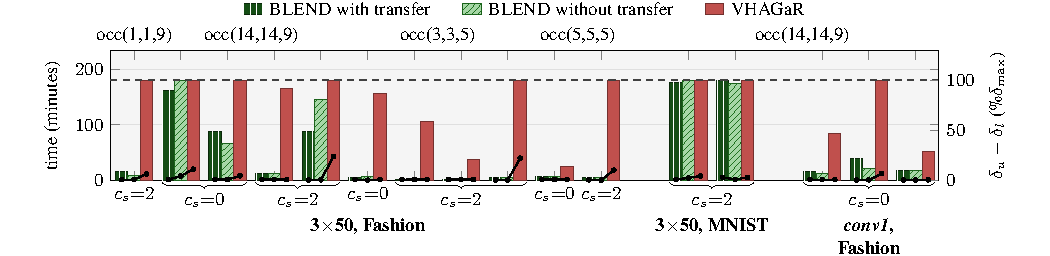
\includegraphics[trim=117 114.731 118 0,clip]{graphics/n2_time_app_6}

\vspace{8pt}

% ===================================================================
% Written by tools/build_time_figures.py -- do not edit by hand.
% One axis for every experiment of this perturbation, rebuilt from
% the numbers of the pdfs the paper generates, in their colours.
% ===================================================================
\definecolor{blendtr}{rgb}{0.083,0.301,0.083}
\definecolor{blendpl}{rgb}{0.652,0.844,0.652}
\definecolor{vhagarcol}{rgb}{0.753,0.314,0.302}
\begin{tikzpicture}[x=1pt,y=1pt,font=\fontsize{9}{10.5}\selectfont]
  \fill[black!3] (0,0) rectangle (296.90,62.50);
  \fill[blendtr] (0.00,0) rectangle (5.50,4.38);
  \draw[black!60,line width=0.2pt] (0.00,0) rectangle (5.50,4.38);
  \fill[blendpl] (5.50,0) rectangle (11.00,2.27);
  \fill[pattern=north east lines,pattern color=blendtr] (5.50,0) rectangle (11.00,2.27);
  \draw[black!60,line width=0.2pt] (5.50,0) rectangle (11.00,2.27);
  \fill[vhagarcol] (11.00,0) rectangle (16.50,48.05);
  \draw[black!60,line width=0.2pt] (11.00,0) rectangle (16.50,48.05);
  \draw[black,line width=0.3pt] (2.75,0.28) -- (8.25,0.30) -- (13.75,3.04);
  \fill[black] (2.75,0.28) circle (0.75pt);
  \fill[black] (8.25,0.30) circle (0.75pt);
  \fill[black] (13.75,3.04) circle (0.75pt);
  \fill[blendtr] (22.50,0) rectangle (28.00,43.17);
  \draw[black!60,line width=0.2pt] (22.50,0) rectangle (28.00,43.17);
  \fill[blendpl] (28.00,0) rectangle (33.50,48.05);
  \fill[pattern=north east lines,pattern color=blendtr] (28.00,0) rectangle (33.50,48.05);
  \draw[black!60,line width=0.2pt] (28.00,0) rectangle (33.50,48.05);
  \fill[vhagarcol] (33.50,0) rectangle (39.00,48.05);
  \draw[black!60,line width=0.2pt] (33.50,0) rectangle (39.00,48.05);
  \draw[black,line width=0.3pt] (25.25,0.31) -- (30.75,2.01) -- (36.25,5.29);
  \fill[black] (25.25,0.31) circle (0.75pt);
  \fill[black] (30.75,2.01) circle (0.75pt);
  \fill[black] (36.25,5.29) circle (0.75pt);
  \fill[blendtr] (43.48,0) rectangle (48.98,23.30);
  \draw[black!60,line width=0.2pt] (43.48,0) rectangle (48.98,23.30);
  \fill[blendpl] (48.98,0) rectangle (54.48,17.42);
  \fill[pattern=north east lines,pattern color=blendtr] (48.98,0) rectangle (54.48,17.42);
  \draw[black!60,line width=0.2pt] (48.98,0) rectangle (54.48,17.42);
  \fill[vhagarcol] (54.48,0) rectangle (59.98,48.05);
  \draw[black!60,line width=0.2pt] (54.48,0) rectangle (59.98,48.05);
  \draw[black,line width=0.3pt] (46.23,0.31) -- (51.73,0.31) -- (57.23,2.09);
  \fill[black] (46.23,0.31) circle (0.75pt);
  \fill[black] (51.73,0.31) circle (0.75pt);
  \fill[black] (57.23,2.09) circle (0.75pt);
  \fill[blendtr] (65.98,0) rectangle (71.48,3.12);
  \draw[black!60,line width=0.2pt] (65.98,0) rectangle (71.48,3.12);
  \fill[blendpl] (71.48,0) rectangle (76.98,3.28);
  \fill[pattern=north east lines,pattern color=blendtr] (71.48,0) rectangle (76.98,3.28);
  \draw[black!60,line width=0.2pt] (71.48,0) rectangle (76.98,3.28);
  \fill[vhagarcol] (76.98,0) rectangle (82.48,44.23);
  \draw[black!60,line width=0.2pt] (76.98,0) rectangle (82.48,44.23);
  \draw[black,line width=0.3pt] (68.73,0.31) -- (74.23,0.30) -- (79.73,0.31);
  \fill[black] (68.73,0.31) circle (0.75pt);
  \fill[black] (74.23,0.30) circle (0.75pt);
  \fill[black] (79.73,0.31) circle (0.75pt);
  \fill[blendtr] (86.96,0) rectangle (92.46,23.17);
  \draw[black!60,line width=0.2pt] (86.96,0) rectangle (92.46,23.17);
  \fill[blendpl] (92.46,0) rectangle (97.96,38.73);
  \fill[pattern=north east lines,pattern color=blendtr] (92.46,0) rectangle (97.96,38.73);
  \draw[black!60,line width=0.2pt] (92.46,0) rectangle (97.96,38.73);
  \fill[vhagarcol] (97.96,0) rectangle (103.46,48.05);
  \draw[black!60,line width=0.2pt] (97.96,0) rectangle (103.46,48.05);
  \draw[black,line width=0.3pt] (89.71,0.17) -- (95.21,0.17) -- (100.71,11.37);
  \fill[black] (89.71,0.17) circle (0.75pt);
  \fill[black] (95.21,0.17) circle (0.75pt);
  \fill[black] (100.71,11.37) circle (0.75pt);
  \fill[blendtr] (109.46,0) rectangle (114.96,1.45);
  \draw[black!60,line width=0.2pt] (109.46,0) rectangle (114.96,1.45);
  \fill[blendpl] (114.96,0) rectangle (120.46,1.62);
  \fill[pattern=north east lines,pattern color=blendtr] (114.96,0) rectangle (120.46,1.62);
  \draw[black!60,line width=0.2pt] (114.96,0) rectangle (120.46,1.62);
  \fill[vhagarcol] (120.46,0) rectangle (125.96,41.78);
  \draw[black!60,line width=0.2pt] (120.46,0) rectangle (125.96,41.78);
  \draw[black,line width=0.3pt] (112.21,0.35) -- (117.71,0.01) -- (123.21,0.36);
  \fill[black] (112.21,0.35) circle (0.75pt);
  \fill[black] (117.71,0.01) circle (0.75pt);
  \fill[black] (123.21,0.36) circle (0.75pt);
  \fill[blendtr] (131.96,0) rectangle (137.46,0.58);
  \draw[black!60,line width=0.2pt] (131.96,0) rectangle (137.46,0.58);
  \fill[blendpl] (137.46,0) rectangle (142.96,0.47);
  \fill[pattern=north east lines,pattern color=blendtr] (137.46,0) rectangle (142.96,0.47);
  \draw[black!60,line width=0.2pt] (137.46,0) rectangle (142.96,0.47);
  \fill[vhagarcol] (142.96,0) rectangle (148.46,27.98);
  \draw[black!60,line width=0.2pt] (142.96,0) rectangle (148.46,27.98);
  \draw[black,line width=0.3pt] (134.71,0.27) -- (140.21,0.34) -- (145.71,0.37);
  \fill[black] (134.71,0.27) circle (0.75pt);
  \fill[black] (140.21,0.34) circle (0.75pt);
  \fill[black] (145.71,0.37) circle (0.75pt);
  \fill[blendtr] (152.94,0) rectangle (158.44,0.38);
  \draw[black!60,line width=0.2pt] (152.94,0) rectangle (158.44,0.38);
  \fill[blendpl] (158.44,0) rectangle (163.94,0.42);
  \fill[pattern=north east lines,pattern color=blendtr] (158.44,0) rectangle (163.94,0.42);
  \draw[black!60,line width=0.2pt] (158.44,0) rectangle (163.94,0.42);
  \fill[vhagarcol] (163.94,0) rectangle (169.44,9.97);
  \draw[black!60,line width=0.2pt] (163.94,0) rectangle (169.44,9.97);
  \draw[black,line width=0.3pt] (155.69,0.31) -- (161.19,0.33) -- (166.69,0.36);
  \fill[black] (155.69,0.31) circle (0.75pt);
  \fill[black] (161.19,0.33) circle (0.75pt);
  \fill[black] (166.69,0.36) circle (0.75pt);
  \fill[blendtr] (175.44,0) rectangle (180.94,1.44);
  \draw[black!60,line width=0.2pt] (175.44,0) rectangle (180.94,1.44);
  \fill[blendpl] (180.94,0) rectangle (186.44,1.35);
  \fill[pattern=north east lines,pattern color=blendtr] (180.94,0) rectangle (186.44,1.35);
  \draw[black!60,line width=0.2pt] (180.94,0) rectangle (186.44,1.35);
  \fill[vhagarcol] (186.44,0) rectangle (191.94,48.05);
  \draw[black!60,line width=0.2pt] (186.44,0) rectangle (191.94,48.05);
  \draw[black,line width=0.3pt] (178.19,0.12) -- (183.69,0.07) -- (189.19,10.60);
  \fill[black] (178.19,0.12) circle (0.75pt);
  \fill[black] (183.69,0.07) circle (0.75pt);
  \fill[black] (189.19,10.60) circle (0.75pt);
  \fill[blendtr] (196.42,0) rectangle (201.92,1.97);
  \draw[black!60,line width=0.2pt] (196.42,0) rectangle (201.92,1.97);
  \fill[blendpl] (201.92,0) rectangle (207.42,1.97);
  \fill[pattern=north east lines,pattern color=blendtr] (201.92,0) rectangle (207.42,1.97);
  \draw[black!60,line width=0.2pt] (201.92,0) rectangle (207.42,1.97);
  \fill[vhagarcol] (207.42,0) rectangle (212.92,6.50);
  \draw[black!60,line width=0.2pt] (207.42,0) rectangle (212.92,6.50);
  \draw[black,line width=0.3pt] (199.17,0.37) -- (204.67,0.38) -- (210.17,0.38);
  \fill[black] (199.17,0.37) circle (0.75pt);
  \fill[black] (204.67,0.38) circle (0.75pt);
  \fill[black] (210.17,0.38) circle (0.75pt);
  \fill[blendtr] (218.92,0) rectangle (224.42,1.36);
  \draw[black!60,line width=0.2pt] (218.92,0) rectangle (224.42,1.36);
  \fill[blendpl] (224.42,0) rectangle (229.92,1.39);
  \fill[pattern=north east lines,pattern color=blendtr] (224.42,0) rectangle (229.92,1.39);
  \draw[black!60,line width=0.2pt] (224.42,0) rectangle (229.92,1.39);
  \fill[vhagarcol] (229.92,0) rectangle (235.42,48.05);
  \draw[black!60,line width=0.2pt] (229.92,0) rectangle (235.42,48.05);
  \draw[black,line width=0.3pt] (221.67,0.22) -- (227.17,0.01) -- (232.67,4.87);
  \fill[black] (221.67,0.22) circle (0.75pt);
  \fill[black] (227.17,0.01) circle (0.75pt);
  \fill[black] (232.67,4.87) circle (0.75pt);
  \fill[blendtr] (259.42,0) rectangle (264.92,46.85);
  \draw[black!60,line width=0.2pt] (259.42,0) rectangle (264.92,46.85);
  \fill[blendpl] (264.92,0) rectangle (270.42,48.05);
  \fill[pattern=north east lines,pattern color=blendtr] (264.92,0) rectangle (270.42,48.05);
  \draw[black!60,line width=0.2pt] (264.92,0) rectangle (270.42,48.05);
  \fill[vhagarcol] (270.42,0) rectangle (275.92,48.05);
  \draw[black!60,line width=0.2pt] (270.42,0) rectangle (275.92,48.05);
  \draw[black,line width=0.3pt] (262.17,0.39) -- (267.67,1.11) -- (273.17,2.08);
  \fill[black] (262.17,0.39) circle (0.75pt);
  \fill[black] (267.67,1.11) circle (0.75pt);
  \fill[black] (273.17,2.08) circle (0.75pt);
  \fill[blendtr] (280.40,0) rectangle (285.90,48.05);
  \draw[black!60,line width=0.2pt] (280.40,0) rectangle (285.90,48.05);
  \fill[blendpl] (285.90,0) rectangle (291.40,46.34);
  \fill[pattern=north east lines,pattern color=blendtr] (285.90,0) rectangle (291.40,46.34);
  \draw[black!60,line width=0.2pt] (285.90,0) rectangle (291.40,46.34);
  \fill[vhagarcol] (291.40,0) rectangle (296.90,48.05);
  \draw[black!60,line width=0.2pt] (291.40,0) rectangle (296.90,48.05);
  \draw[black,line width=0.3pt] (283.15,1.35) -- (288.65,0.39) -- (294.15,1.32);
  \fill[black] (283.15,1.35) circle (0.75pt);
  \fill[black] (288.65,0.39) circle (0.75pt);
  \fill[black] (294.15,1.32) circle (0.75pt);
  \draw[black!60,line width=0.3pt] (0,0) rectangle (296.90,62.50);
  \draw[black,dashed,line width=0.3pt] (0,48.05) -- (296.90,48.05);
  \draw[black!60,line width=0.3pt] (0,0.00) -- (-2,0.00) node[left,inner sep=1pt,font=\fontsize{10.95}{13}\selectfont] {0};
  \draw[black!60,line width=0.3pt] (0,26.69) -- (-2,26.69) node[left,inner sep=1pt,font=\fontsize{10.95}{13}\selectfont] {100};
  \draw[black!60,line width=0.3pt] (0,53.39) -- (-2,53.39) node[left,inner sep=1pt,font=\fontsize{10.95}{13}\selectfont] {200};
  \node[rotate=90,anchor=south,font=\fontsize{10.95}{13}\selectfont] at (-26.0,31.25) {time (minutes)};
  \draw[black!60,line width=0.3pt] (296.90,0.00) -- (298.90,0.00) node[right,inner sep=1pt,font=\fontsize{10.95}{13}\selectfont] {0};
  \draw[black!60,line width=0.3pt] (296.90,24.02) -- (298.90,24.02) node[right,inner sep=1pt,font=\fontsize{10.95}{13}\selectfont] {50};
  \draw[black!60,line width=0.3pt] (296.90,48.05) -- (298.90,48.05) node[right,inner sep=1pt,font=\fontsize{10.95}{13}\selectfont] {100};
  \node[rotate=90,anchor=north,font=\fontsize{10.95}{13}\selectfont] at (322.90,31.25) {$\delta_u-\delta_l$ (\%$\delta_{\max}$)};
  \node[above,inner sep=1.5pt,font=\fontsize{10.95}{13}\selectfont] at (148.45,77.00) {occlusion};
  \draw[black,line width=0.25pt] (0.00,64.00) -- (0.00,65.50) -- (39.00,65.50) -- (39.00,64.00);
  \node[above,inner sep=1.5pt,font=\fontsize{9}{10.5}\selectfont] at (19.50,65.50) {(1,1,9)};
  \draw[black,line width=0.25pt] (43.48,64.00) -- (43.48,65.50) -- (103.46,65.50) -- (103.46,64.00);
  \node[above,inner sep=1.5pt,font=\fontsize{9}{10.5}\selectfont] at (73.47,65.50) {(14,14,9)};
  \draw[black,line width=0.25pt] (109.46,64.00) -- (109.46,65.50) -- (169.44,65.50) -- (169.44,64.00);
  \node[above,inner sep=1.5pt,font=\fontsize{9}{10.5}\selectfont] at (139.45,65.50) {(3,3,5)};
  \draw[black,line width=0.25pt] (175.44,64.00) -- (175.44,65.50) -- (235.42,65.50) -- (235.42,64.00);
  \node[above,inner sep=1.5pt,font=\fontsize{9}{10.5}\selectfont] at (205.43,65.50) {(5,5,5)};
  \draw[black,line width=0.25pt] (259.42,64.00) -- (259.42,65.50) -- (296.90,65.50) -- (296.90,64.00);
  \node[above,inner sep=1.5pt,font=\fontsize{9}{10.5}\selectfont] at (278.16,65.50) {(14,14,9)};
  \draw[black,line width=0.25pt] (0.00,-1.5) -- (0.00,-3) -- (16.50,-3) -- (16.50,-1.5);
  \node[below,inner sep=1.5pt,font=\fontsize{9}{10.5}\selectfont] at (8.25,-3) {$c_s{=}2$};
  \draw[black,line width=0.25pt] (22.50,-1.5) -- (22.50,-3) -- (59.98,-3) -- (59.98,-1.5);
  \node[below,inner sep=1.5pt,font=\fontsize{9}{10.5}\selectfont] at (41.24,-3) {$c_s{=}0$};
  \draw[black,line width=0.25pt] (65.98,-1.5) -- (65.98,-3) -- (103.46,-3) -- (103.46,-1.5);
  \node[below,inner sep=1.5pt,font=\fontsize{9}{10.5}\selectfont] at (84.72,-3) {$c_s{=}2$};
  \draw[black,line width=0.25pt] (109.46,-1.5) -- (109.46,-3) -- (125.96,-3) -- (125.96,-1.5);
  \node[below,inner sep=1.5pt,font=\fontsize{9}{10.5}\selectfont] at (117.71,-3) {$c_s{=}0$};
  \draw[black,line width=0.25pt] (131.96,-1.5) -- (131.96,-3) -- (169.44,-3) -- (169.44,-1.5);
  \node[below,inner sep=1.5pt,font=\fontsize{9}{10.5}\selectfont] at (150.70,-3) {$c_s{=}2$};
  \draw[black,line width=0.25pt] (175.44,-1.5) -- (175.44,-3) -- (212.92,-3) -- (212.92,-1.5);
  \node[below,inner sep=1.5pt,font=\fontsize{9}{10.5}\selectfont] at (194.18,-3) {$c_s{=}0$};
  \draw[black,line width=0.25pt] (218.92,-1.5) -- (218.92,-3) -- (235.42,-3) -- (235.42,-1.5);
  \node[below,inner sep=1.5pt,font=\fontsize{9}{10.5}\selectfont] at (227.17,-3) {$c_s{=}2$};
  \draw[black,line width=0.25pt] (259.42,-1.5) -- (259.42,-3) -- (296.90,-3) -- (296.90,-1.5);
  \node[below,inner sep=1.5pt,font=\fontsize{9}{10.5}\selectfont] at (278.16,-3) {$c_s{=}2$};
  \node[below,align=center,inner sep=1pt,font=\fontsize{9}{10.5}\selectfont\bfseries] at (117.71,-15.00) {3$\times$50\\FMNIST};
  \node[below,align=center,inner sep=1pt,font=\fontsize{9}{10.5}\selectfont\bfseries] at (278.16,-15.00) {3$\times$50\\MNIST};
\end{tikzpicture}


\vspace{8pt}

% ===================================================================
% Written by tools/build_time_figures.py -- do not edit by hand.
% One axis for every experiment of this perturbation, rebuilt from
% the numbers of the pdfs the paper generates, in their colours.
% ===================================================================
\definecolor{blendtr}{rgb}{0.083,0.301,0.083}
\definecolor{blendpl}{rgb}{0.652,0.844,0.652}
\definecolor{vhagarcol}{rgb}{0.753,0.314,0.302}
\begin{tikzpicture}[x=1pt,y=1pt,font=\fontsize{9}{10.5}\selectfont]
  \fill[black!3] (0,0) rectangle (321.00,62.50);
  \fill[blendtr] (0.00,0) rectangle (5.49,4.34);
  \draw[black!60,line width=0.2pt] (0.00,0) rectangle (5.49,4.34);
  \fill[blendpl] (5.49,0) rectangle (10.98,3.37);
  \fill[pattern=north east lines,pattern color=blendtr] (5.49,0) rectangle (10.98,3.37);
  \draw[black!60,line width=0.2pt] (5.49,0) rectangle (10.98,3.37);
  \fill[vhagarcol] (10.98,0) rectangle (16.48,22.63);
  \draw[black!60,line width=0.2pt] (10.98,0) rectangle (16.48,22.63);
  \draw[black,line width=0.3pt] (2.75,0.29) -- (8.24,0.26) -- (13.73,0.30);
  \fill[black] (2.75,0.29) circle (0.75pt);
  \fill[black] (8.24,0.26) circle (0.75pt);
  \fill[black] (13.73,0.30) circle (0.75pt);
  \fill[blendtr] (20.96,0) rectangle (26.45,10.36);
  \draw[black!60,line width=0.2pt] (20.96,0) rectangle (26.45,10.36);
  \fill[blendpl] (26.45,0) rectangle (31.94,5.46);
  \fill[pattern=north east lines,pattern color=blendtr] (26.45,0) rectangle (31.94,5.46);
  \draw[black!60,line width=0.2pt] (26.45,0) rectangle (31.94,5.46);
  \fill[vhagarcol] (31.94,0) rectangle (37.43,48.05);
  \draw[black!60,line width=0.2pt] (31.94,0) rectangle (37.43,48.05);
  \draw[black,line width=0.3pt] (23.70,0.13) -- (29.20,0.15) -- (34.69,3.18);
  \fill[black] (23.70,0.13) circle (0.75pt);
  \fill[black] (29.20,0.15) circle (0.75pt);
  \fill[black] (34.69,3.18) circle (0.75pt);
  \fill[blendtr] (41.91,0) rectangle (47.41,4.77);
  \draw[black!60,line width=0.2pt] (41.91,0) rectangle (47.41,4.77);
  \fill[blendpl] (47.41,0) rectangle (52.90,4.77);
  \fill[pattern=north east lines,pattern color=blendtr] (47.41,0) rectangle (52.90,4.77);
  \draw[black!60,line width=0.2pt] (47.41,0) rectangle (52.90,4.77);
  \fill[vhagarcol] (52.90,0) rectangle (58.39,13.78);
  \draw[black!60,line width=0.2pt] (52.90,0) rectangle (58.39,13.78);
  \draw[black,line width=0.3pt] (44.66,0.16) -- (50.15,0.16) -- (55.65,0.18);
  \fill[black] (44.66,0.16) circle (0.75pt);
  \fill[black] (50.15,0.16) circle (0.75pt);
  \fill[black] (55.65,0.18) circle (0.75pt);
  \fill[blendtr] (64.39,0) rectangle (69.88,0.78);
  \draw[black!60,line width=0.2pt] (64.39,0) rectangle (69.88,0.78);
  \fill[blendpl] (69.88,0) rectangle (75.38,1.27);
  \fill[pattern=north east lines,pattern color=blendtr] (69.88,0) rectangle (75.38,1.27);
  \draw[black!60,line width=0.2pt] (69.88,0) rectangle (75.38,1.27);
  \fill[vhagarcol] (75.38,0) rectangle (80.87,8.81);
  \draw[black!60,line width=0.2pt] (75.38,0) rectangle (80.87,8.81);
  \draw[black,line width=0.3pt] (67.14,0.42) -- (72.63,0.36) -- (78.12,0.41);
  \fill[black] (67.14,0.42) circle (0.75pt);
  \fill[black] (72.63,0.36) circle (0.75pt);
  \fill[black] (78.12,0.41) circle (0.75pt);
  \fill[blendtr] (85.35,0) rectangle (90.84,18.76);
  \draw[black!60,line width=0.2pt] (85.35,0) rectangle (90.84,18.76);
  \fill[blendpl] (90.84,0) rectangle (96.33,16.56);
  \fill[pattern=north east lines,pattern color=blendtr] (90.84,0) rectangle (96.33,16.56);
  \draw[black!60,line width=0.2pt] (90.84,0) rectangle (96.33,16.56);
  \fill[vhagarcol] (96.33,0) rectangle (101.83,48.05);
  \draw[black!60,line width=0.2pt] (96.33,0) rectangle (101.83,48.05);
  \draw[black,line width=0.3pt] (88.10,0.27) -- (93.59,0.28) -- (99.08,3.71);
  \fill[black] (88.10,0.27) circle (0.75pt);
  \fill[black] (93.59,0.28) circle (0.75pt);
  \fill[black] (99.08,3.71) circle (0.75pt);
  \fill[blendtr] (106.31,0) rectangle (111.80,41.08);
  \draw[black!60,line width=0.2pt] (106.31,0) rectangle (111.80,41.08);
  \fill[blendpl] (111.80,0) rectangle (117.29,20.33);
  \fill[pattern=north east lines,pattern color=blendtr] (111.80,0) rectangle (117.29,20.33);
  \draw[black!60,line width=0.2pt] (111.80,0) rectangle (117.29,20.33);
  \fill[vhagarcol] (117.29,0) rectangle (122.78,48.05);
  \draw[black!60,line width=0.2pt] (117.29,0) rectangle (122.78,48.05);
  \draw[black,line width=0.3pt] (109.05,0.33) -- (114.55,0.33) -- (120.04,7.77);
  \fill[black] (109.05,0.33) circle (0.75pt);
  \fill[black] (114.55,0.33) circle (0.75pt);
  \fill[black] (120.04,7.77) circle (0.75pt);
  \fill[blendtr] (127.26,0) rectangle (132.76,0.15);
  \draw[black!60,line width=0.2pt] (127.26,0) rectangle (132.76,0.15);
  \fill[blendpl] (132.76,0) rectangle (138.25,0.14);
  \fill[pattern=north east lines,pattern color=blendtr] (132.76,0) rectangle (138.25,0.14);
  \draw[black!60,line width=0.2pt] (132.76,0) rectangle (138.25,0.14);
  \fill[vhagarcol] (138.25,0) rectangle (143.74,11.16);
  \draw[black!60,line width=0.2pt] (138.25,0) rectangle (143.74,11.16);
  \draw[black,line width=0.3pt] (130.01,0.23) -- (135.50,0.22) -- (141.00,0.19);
  \fill[black] (130.01,0.23) circle (0.75pt);
  \fill[black] (135.50,0.22) circle (0.75pt);
  \fill[black] (141.00,0.19) circle (0.75pt);
  \fill[blendtr] (148.22,0) rectangle (153.71,0.31);
  \draw[black!60,line width=0.2pt] (148.22,0) rectangle (153.71,0.31);
  \fill[blendpl] (153.71,0) rectangle (159.21,0.28);
  \fill[pattern=north east lines,pattern color=blendtr] (153.71,0) rectangle (159.21,0.28);
  \draw[black!60,line width=0.2pt] (153.71,0) rectangle (159.21,0.28);
  \fill[vhagarcol] (159.21,0) rectangle (164.70,9.51);
  \draw[black!60,line width=0.2pt] (159.21,0) rectangle (164.70,9.51);
  \draw[black,line width=0.3pt] (150.97,0.30) -- (156.46,0.35) -- (161.95,0.34);
  \fill[black] (150.97,0.30) circle (0.75pt);
  \fill[black] (156.46,0.35) circle (0.75pt);
  \fill[black] (161.95,0.34) circle (0.75pt);
  \fill[blendtr] (169.18,0) rectangle (174.67,0.49);
  \draw[black!60,line width=0.2pt] (169.18,0) rectangle (174.67,0.49);
  \fill[blendpl] (174.67,0) rectangle (180.16,0.78);
  \fill[pattern=north east lines,pattern color=blendtr] (174.67,0) rectangle (180.16,0.78);
  \draw[black!60,line width=0.2pt] (174.67,0) rectangle (180.16,0.78);
  \fill[vhagarcol] (180.16,0) rectangle (185.66,7.20);
  \draw[black!60,line width=0.2pt] (180.16,0) rectangle (185.66,7.20);
  \draw[black,line width=0.3pt] (171.92,0.27) -- (177.42,0.30) -- (182.91,0.33);
  \fill[black] (171.92,0.27) circle (0.75pt);
  \fill[black] (177.42,0.30) circle (0.75pt);
  \fill[black] (182.91,0.33) circle (0.75pt);
  \fill[blendtr] (193.66,0) rectangle (199.15,0.17);
  \draw[black!60,line width=0.2pt] (193.66,0) rectangle (199.15,0.17);
  \fill[blendpl] (199.15,0) rectangle (204.64,0.19);
  \fill[pattern=north east lines,pattern color=blendtr] (199.15,0) rectangle (204.64,0.19);
  \draw[black!60,line width=0.2pt] (199.15,0) rectangle (204.64,0.19);
  \fill[vhagarcol] (204.64,0) rectangle (210.13,14.78);
  \draw[black!60,line width=0.2pt] (204.64,0) rectangle (210.13,14.78);
  \draw[black,line width=0.3pt] (196.40,0.09) -- (201.89,0.09) -- (207.39,0.10);
  \fill[black] (196.40,0.09) circle (0.75pt);
  \fill[black] (201.89,0.09) circle (0.75pt);
  \fill[black] (207.39,0.10) circle (0.75pt);
  \fill[blendtr] (216.13,0) rectangle (221.63,0.20);
  \draw[black!60,line width=0.2pt] (216.13,0) rectangle (221.63,0.20);
  \fill[blendpl] (221.63,0) rectangle (227.12,0.26);
  \fill[pattern=north east lines,pattern color=blendtr] (221.63,0) rectangle (227.12,0.26);
  \draw[black!60,line width=0.2pt] (221.63,0) rectangle (227.12,0.26);
  \fill[vhagarcol] (227.12,0) rectangle (232.61,48.05);
  \draw[black!60,line width=0.2pt] (227.12,0) rectangle (232.61,48.05);
  \draw[black,line width=0.3pt] (218.88,0.04) -- (224.37,0.00) -- (229.86,13.84);
  \fill[black] (218.88,0.04) circle (0.75pt);
  \fill[black] (224.37,0.00) circle (0.75pt);
  \fill[black] (229.86,13.84) circle (0.75pt);
  \fill[blendtr] (238.61,0) rectangle (244.10,0.12);
  \draw[black!60,line width=0.2pt] (238.61,0) rectangle (244.10,0.12);
  \fill[blendpl] (244.10,0) rectangle (249.60,4.27);
  \fill[pattern=north east lines,pattern color=blendtr] (244.10,0) rectangle (249.60,4.27);
  \draw[black!60,line width=0.2pt] (244.10,0) rectangle (249.60,4.27);
  \fill[vhagarcol] (249.60,0) rectangle (255.09,2.49);
  \draw[black!60,line width=0.2pt] (249.60,0) rectangle (255.09,2.49);
  \draw[black,line width=0.3pt] (241.36,0.13) -- (246.85,0.08) -- (252.34,0.12);
  \fill[black] (241.36,0.13) circle (0.75pt);
  \fill[black] (246.85,0.08) circle (0.75pt);
  \fill[black] (252.34,0.12) circle (0.75pt);
  \fill[blendtr] (259.57,0) rectangle (265.06,0.14);
  \draw[black!60,line width=0.2pt] (259.57,0) rectangle (265.06,0.14);
  \fill[blendpl] (265.06,0) rectangle (270.55,0.17);
  \fill[pattern=north east lines,pattern color=blendtr] (265.06,0) rectangle (270.55,0.17);
  \draw[black!60,line width=0.2pt] (265.06,0) rectangle (270.55,0.17);
  \fill[vhagarcol] (270.55,0) rectangle (276.05,48.05);
  \draw[black!60,line width=0.2pt] (270.55,0) rectangle (276.05,48.05);
  \draw[black,line width=0.3pt] (262.31,0.17) -- (267.81,0.20) -- (273.30,10.11);
  \fill[black] (262.31,0.17) circle (0.75pt);
  \fill[black] (267.81,0.20) circle (0.75pt);
  \fill[black] (273.30,10.11) circle (0.75pt);
  \fill[blendtr] (282.05,0) rectangle (287.54,0.16);
  \draw[black!60,line width=0.2pt] (282.05,0) rectangle (287.54,0.16);
  \fill[blendpl] (287.54,0) rectangle (293.03,0.62);
  \fill[pattern=north east lines,pattern color=blendtr] (287.54,0) rectangle (293.03,0.62);
  \draw[black!60,line width=0.2pt] (287.54,0) rectangle (293.03,0.62);
  \fill[vhagarcol] (293.03,0) rectangle (298.52,4.98);
  \draw[black!60,line width=0.2pt] (293.03,0) rectangle (298.52,4.98);
  \draw[black,line width=0.3pt] (284.79,0.00) -- (290.28,0.15) -- (295.78,0.18);
  \fill[black] (284.79,0.00) circle (0.75pt);
  \fill[black] (290.28,0.15) circle (0.75pt);
  \fill[black] (295.78,0.18) circle (0.75pt);
  \fill[blendtr] (304.52,0) rectangle (310.02,0.13);
  \draw[black!60,line width=0.2pt] (304.52,0) rectangle (310.02,0.13);
  \fill[blendpl] (310.02,0) rectangle (315.51,16.10);
  \fill[pattern=north east lines,pattern color=blendtr] (310.02,0) rectangle (315.51,16.10);
  \draw[black!60,line width=0.2pt] (310.02,0) rectangle (315.51,16.10);
  \fill[vhagarcol] (315.51,0) rectangle (321.00,1.37);
  \draw[black!60,line width=0.2pt] (315.51,0) rectangle (321.00,1.37);
  \draw[black,line width=0.3pt] (307.27,0.05) -- (312.76,0.03) -- (318.25,0.00);
  \fill[black] (307.27,0.05) circle (0.75pt);
  \fill[black] (312.76,0.03) circle (0.75pt);
  \fill[black] (318.25,0.00) circle (0.75pt);
  \draw[black!60,line width=0.3pt] (0,0) rectangle (321.00,62.50);
  \draw[black,dashed,line width=0.3pt] (0,48.05) -- (321.00,48.05);
  \draw[black!60,line width=0.3pt] (0,0.00) -- (-2,0.00) node[left,inner sep=1pt,font=\fontsize{10.95}{13}\selectfont] {0};
  \draw[black!60,line width=0.3pt] (0,26.69) -- (-2,26.69) node[left,inner sep=1pt,font=\fontsize{10.95}{13}\selectfont] {100};
  \draw[black!60,line width=0.3pt] (0,53.39) -- (-2,53.39) node[left,inner sep=1pt,font=\fontsize{10.95}{13}\selectfont] {200};
  \node[rotate=90,anchor=south,font=\fontsize{10.95}{13}\selectfont] at (-26.0,31.25) {time (minutes)};
  \draw[black!60,line width=0.3pt] (321.00,0.00) -- (323.00,0.00) node[right,inner sep=1pt,font=\fontsize{10.95}{13}\selectfont] {0};
  \draw[black!60,line width=0.3pt] (321.00,24.02) -- (323.00,24.02) node[right,inner sep=1pt,font=\fontsize{10.95}{13}\selectfont] {50};
  \draw[black!60,line width=0.3pt] (321.00,48.05) -- (323.00,48.05) node[right,inner sep=1pt,font=\fontsize{10.95}{13}\selectfont] {100};
  \node[rotate=90,anchor=north,font=\fontsize{10.95}{13}\selectfont] at (347.00,31.25) {$\delta_u-\delta_l$ (\%$\delta_{\max}$)};
  \node[above,inner sep=1.5pt,font=\fontsize{10.95}{13}\selectfont] at (160.50,77.00) {occlusion};
  \draw[black,line width=0.25pt] (0.00,64.00) -- (0.00,65.50) -- (122.78,65.50) -- (122.78,64.00);
  \node[above,inner sep=1.5pt,font=\fontsize{9}{10.5}\selectfont] at (61.39,65.50) {(14,14,9)};
  \draw[black,line width=0.25pt] (127.26,64.00) -- (127.26,65.50) -- (185.66,65.50) -- (185.66,64.00);
  \node[above,inner sep=1.5pt,font=\fontsize{9}{10.5}\selectfont] at (156.46,65.50) {(3,3,5)};
  \draw[black,line width=0.25pt] (193.66,64.00) -- (193.66,65.50) -- (232.61,65.50) -- (232.61,64.00);
  \node[above,inner sep=1.5pt,font=\fontsize{9}{10.5}\selectfont] at (213.13,65.50) {(1,1,5)};
  \draw[black,line width=0.25pt] (238.61,64.00) -- (238.61,65.50) -- (321.00,65.50) -- (321.00,64.00);
  \node[above,inner sep=1.5pt,font=\fontsize{9}{10.5}\selectfont] at (279.81,65.50) {(1,1,9)};
  \draw[black,line width=0.25pt] (0.00,-1.5) -- (0.00,-3) -- (58.39,-3) -- (58.39,-1.5);
  \node[below,inner sep=1.5pt,font=\fontsize{9}{10.5}\selectfont] at (29.20,-3) {$c_s{=}0$};
  \draw[black,line width=0.25pt] (64.39,-1.5) -- (64.39,-3) -- (185.66,-3) -- (185.66,-1.5);
  \node[below,inner sep=1.5pt,font=\fontsize{9}{10.5}\selectfont] at (125.02,-3) {$c_s{=}2$};
  \draw[black,line width=0.25pt] (193.66,-1.5) -- (193.66,-3) -- (210.13,-3) -- (210.13,-1.5);
  \node[below,inner sep=1.5pt,font=\fontsize{9}{10.5}\selectfont] at (201.89,-3) {$c_s{=}0$};
  \draw[black,line width=0.25pt] (216.13,-1.5) -- (216.13,-3) -- (232.61,-3) -- (232.61,-1.5);
  \node[below,inner sep=1.5pt,font=\fontsize{9}{10.5}\selectfont] at (224.37,-3) {$c_s{=}1$};
  \draw[black,line width=0.25pt] (238.61,-1.5) -- (238.61,-3) -- (276.05,-3) -- (276.05,-1.5);
  \node[below,inner sep=1.5pt,font=\fontsize{9}{10.5}\selectfont] at (257.33,-3) {$c_s{=}0$};
  \draw[black,line width=0.25pt] (282.05,-1.5) -- (282.05,-3) -- (298.52,-3) -- (298.52,-1.5);
  \node[below,inner sep=1.5pt,font=\fontsize{9}{10.5}\selectfont] at (290.28,-3) {$c_s{=}1$};
  \draw[black,line width=0.25pt] (304.52,-1.5) -- (304.52,-3) -- (321.00,-3) -- (321.00,-1.5);
  \node[below,inner sep=1.5pt,font=\fontsize{9}{10.5}\selectfont] at (312.76,-3) {$c_s{=}2$};
  \node[below,align=center,inner sep=1pt,font=\fontsize{9}{10.5}\selectfont\bfseries] at (92.83,-15.00) {\emph{conv1}\\FMNIST};
  \node[below,align=center,inner sep=1pt,font=\fontsize{9}{10.5}\selectfont\bfseries] at (257.33,-15.00) {\emph{conv1}\\MNIST};
\end{tikzpicture}


\vspace{8pt}

% ===================================================================
% Written by tools/build_time_figures.py -- do not edit by hand.
% One axis for every experiment of this perturbation, rebuilt from
% the numbers of the pdfs the paper generates, in their colours.
% ===================================================================
\definecolor{blendtr}{rgb}{0.083,0.301,0.083}
\definecolor{blendpl}{rgb}{0.652,0.844,0.652}
\definecolor{vhagarcol}{rgb}{0.753,0.314,0.302}
\begin{tikzpicture}[x=1pt,y=1pt,font=\fontsize{9}{10.5}\selectfont]
  \fill[black!3] (0,0) rectangle (319.40,62.50);
  \fill[blendtr] (0.00,0) rectangle (5.50,40.63);
  \draw[black!60,line width=0.2pt] (0.00,0) rectangle (5.50,40.63);
  \fill[blendpl] (5.50,0) rectangle (11.00,43.06);
  \fill[pattern=north east lines,pattern color=blendtr] (5.50,0) rectangle (11.00,43.06);
  \draw[black!60,line width=0.2pt] (5.50,0) rectangle (11.00,43.06);
  \fill[vhagarcol] (11.00,0) rectangle (16.50,48.05);
  \draw[black!60,line width=0.2pt] (11.00,0) rectangle (16.50,48.05);
  \draw[black,line width=0.3pt] (2.75,0.19) -- (8.25,0.19) -- (13.75,24.65);
  \fill[black] (2.75,0.19) circle (0.75pt);
  \fill[black] (8.25,0.19) circle (0.75pt);
  \fill[black] (13.75,24.65) circle (0.75pt);
  \fill[blendtr] (20.98,0) rectangle (26.48,48.05);
  \draw[black!60,line width=0.2pt] (20.98,0) rectangle (26.48,48.05);
  \fill[blendpl] (26.48,0) rectangle (31.98,43.62);
  \fill[pattern=north east lines,pattern color=blendtr] (26.48,0) rectangle (31.98,43.62);
  \draw[black!60,line width=0.2pt] (26.48,0) rectangle (31.98,43.62);
  \fill[vhagarcol] (31.98,0) rectangle (37.48,48.05);
  \draw[black!60,line width=0.2pt] (31.98,0) rectangle (37.48,48.05);
  \draw[black,line width=0.3pt] (23.73,0.54) -- (29.23,0.14) -- (34.73,34.40);
  \fill[black] (23.73,0.54) circle (0.75pt);
  \fill[black] (29.23,0.14) circle (0.75pt);
  \fill[black] (34.73,34.40) circle (0.75pt);
  \fill[blendtr] (43.48,0) rectangle (48.98,48.05);
  \draw[black!60,line width=0.2pt] (43.48,0) rectangle (48.98,48.05);
  \fill[blendpl] (48.98,0) rectangle (54.48,33.29);
  \fill[pattern=north east lines,pattern color=blendtr] (48.98,0) rectangle (54.48,33.29);
  \draw[black!60,line width=0.2pt] (48.98,0) rectangle (54.48,33.29);
  \fill[vhagarcol] (54.48,0) rectangle (59.98,48.05);
  \draw[black!60,line width=0.2pt] (54.48,0) rectangle (59.98,48.05);
  \draw[black,line width=0.3pt] (46.23,28.28) -- (51.73,0.18) -- (57.23,29.72);
  \fill[black] (46.23,28.28) circle (0.75pt);
  \fill[black] (51.73,0.18) circle (0.75pt);
  \fill[black] (57.23,29.72) circle (0.75pt);
  \fill[blendtr] (65.98,0) rectangle (71.48,29.52);
  \draw[black!60,line width=0.2pt] (65.98,0) rectangle (71.48,29.52);
  \fill[blendpl] (71.48,0) rectangle (76.98,35.26);
  \fill[pattern=north east lines,pattern color=blendtr] (71.48,0) rectangle (76.98,35.26);
  \draw[black!60,line width=0.2pt] (71.48,0) rectangle (76.98,35.26);
  \fill[vhagarcol] (76.98,0) rectangle (82.48,48.05);
  \draw[black!60,line width=0.2pt] (76.98,0) rectangle (82.48,48.05);
  \draw[black,line width=0.3pt] (68.73,0.18) -- (74.23,0.19) -- (79.73,4.64);
  \fill[black] (68.73,0.18) circle (0.75pt);
  \fill[black] (74.23,0.19) circle (0.75pt);
  \fill[black] (79.73,4.64) circle (0.75pt);
  \fill[blendtr] (88.48,0) rectangle (93.98,0.14);
  \draw[black!60,line width=0.2pt] (88.48,0) rectangle (93.98,0.14);
  \fill[blendpl] (93.98,0) rectangle (99.48,48.05);
  \fill[pattern=north east lines,pattern color=blendtr] (93.98,0) rectangle (99.48,48.05);
  \draw[black!60,line width=0.2pt] (93.98,0) rectangle (99.48,48.05);
  \fill[vhagarcol] (99.48,0) rectangle (104.98,15.59);
  \draw[black!60,line width=0.2pt] (99.48,0) rectangle (104.98,15.59);
  \draw[black,line width=0.3pt] (91.23,0.00) -- (96.73,1.05) -- (102.23,0.10);
  \fill[black] (91.23,0.00) circle (0.75pt);
  \fill[black] (96.73,1.05) circle (0.75pt);
  \fill[black] (102.23,0.10) circle (0.75pt);
  \fill[blendtr] (110.98,0) rectangle (116.48,0.49);
  \draw[black!60,line width=0.2pt] (110.98,0) rectangle (116.48,0.49);
  \fill[blendpl] (116.48,0) rectangle (121.98,0.85);
  \fill[pattern=north east lines,pattern color=blendtr] (116.48,0) rectangle (121.98,0.85);
  \draw[black!60,line width=0.2pt] (116.48,0) rectangle (121.98,0.85);
  \fill[vhagarcol] (121.98,0) rectangle (127.48,47.73);
  \draw[black!60,line width=0.2pt] (121.98,0) rectangle (127.48,47.73);
  \draw[black,line width=0.3pt] (113.73,0.03) -- (119.23,0.02) -- (124.73,0.02);
  \fill[black] (113.73,0.03) circle (0.75pt);
  \fill[black] (119.23,0.02) circle (0.75pt);
  \fill[black] (124.73,0.02) circle (0.75pt);
  \fill[blendtr] (131.96,0) rectangle (137.46,1.03);
  \draw[black!60,line width=0.2pt] (131.96,0) rectangle (137.46,1.03);
  \fill[blendpl] (137.46,0) rectangle (142.96,2.00);
  \fill[pattern=north east lines,pattern color=blendtr] (137.46,0) rectangle (142.96,2.00);
  \draw[black!60,line width=0.2pt] (137.46,0) rectangle (142.96,2.00);
  \fill[vhagarcol] (142.96,0) rectangle (148.46,4.69);
  \draw[black!60,line width=0.2pt] (142.96,0) rectangle (148.46,4.69);
  \draw[black,line width=0.3pt] (134.71,0.03) -- (140.21,0.02) -- (145.71,0.03);
  \fill[black] (134.71,0.03) circle (0.75pt);
  \fill[black] (140.21,0.02) circle (0.75pt);
  \fill[black] (145.71,0.03) circle (0.75pt);
  \fill[blendtr] (154.46,0) rectangle (159.96,0.25);
  \draw[black!60,line width=0.2pt] (154.46,0) rectangle (159.96,0.25);
  \fill[blendpl] (159.96,0) rectangle (165.46,0.19);
  \fill[pattern=north east lines,pattern color=blendtr] (159.96,0) rectangle (165.46,0.19);
  \draw[black!60,line width=0.2pt] (159.96,0) rectangle (165.46,0.19);
  \fill[vhagarcol] (165.46,0) rectangle (170.96,34.57);
  \draw[black!60,line width=0.2pt] (165.46,0) rectangle (170.96,34.57);
  \draw[black,line width=0.3pt] (157.21,0.07) -- (162.71,0.00) -- (168.21,0.10);
  \fill[black] (157.21,0.07) circle (0.75pt);
  \fill[black] (162.71,0.00) circle (0.75pt);
  \fill[black] (168.21,0.10) circle (0.75pt);
  \fill[blendtr] (175.44,0) rectangle (180.94,48.05);
  \draw[black!60,line width=0.2pt] (175.44,0) rectangle (180.94,48.05);
  \fill[blendpl] (180.94,0) rectangle (186.44,1.43);
  \fill[pattern=north east lines,pattern color=blendtr] (180.94,0) rectangle (186.44,1.43);
  \draw[black!60,line width=0.2pt] (180.94,0) rectangle (186.44,1.43);
  \fill[vhagarcol] (186.44,0) rectangle (191.94,7.16);
  \draw[black!60,line width=0.2pt] (186.44,0) rectangle (191.94,7.16);
  \draw[black,line width=0.3pt] (178.19,3.55) -- (183.69,0.06) -- (189.19,0.08);
  \fill[black] (178.19,3.55) circle (0.75pt);
  \fill[black] (183.69,0.06) circle (0.75pt);
  \fill[black] (189.19,0.08) circle (0.75pt);
  \fill[blendtr] (197.94,0) rectangle (203.44,0.14);
  \draw[black!60,line width=0.2pt] (197.94,0) rectangle (203.44,0.14);
  \fill[blendpl] (203.44,0) rectangle (208.94,0.13);
  \fill[pattern=north east lines,pattern color=blendtr] (203.44,0) rectangle (208.94,0.13);
  \draw[black!60,line width=0.2pt] (203.44,0) rectangle (208.94,0.13);
  \fill[vhagarcol] (208.94,0) rectangle (214.44,16.32);
  \draw[black!60,line width=0.2pt] (208.94,0) rectangle (214.44,16.32);
  \draw[black,line width=0.3pt] (200.69,0.03) -- (206.19,0.00) -- (211.69,0.02);
  \fill[black] (200.69,0.03) circle (0.75pt);
  \fill[black] (206.19,0.00) circle (0.75pt);
  \fill[black] (211.69,0.02) circle (0.75pt);
  \fill[blendtr] (220.44,0) rectangle (225.94,0.30);
  \draw[black!60,line width=0.2pt] (220.44,0) rectangle (225.94,0.30);
  \fill[blendpl] (225.94,0) rectangle (231.44,0.28);
  \fill[pattern=north east lines,pattern color=blendtr] (225.94,0) rectangle (231.44,0.28);
  \draw[black!60,line width=0.2pt] (225.94,0) rectangle (231.44,0.28);
  \fill[vhagarcol] (231.44,0) rectangle (236.94,5.25);
  \draw[black!60,line width=0.2pt] (231.44,0) rectangle (236.94,5.25);
  \draw[black,line width=0.3pt] (223.19,0.13) -- (228.69,0.07) -- (234.19,0.12);
  \fill[black] (223.19,0.13) circle (0.75pt);
  \fill[black] (228.69,0.07) circle (0.75pt);
  \fill[black] (234.19,0.12) circle (0.75pt);
  \fill[blendtr] (260.94,0) rectangle (266.44,18.03);
  \draw[black!60,line width=0.2pt] (260.94,0) rectangle (266.44,18.03);
  \fill[blendpl] (266.44,0) rectangle (271.94,48.05);
  \fill[pattern=north east lines,pattern color=blendtr] (266.44,0) rectangle (271.94,48.05);
  \draw[black!60,line width=0.2pt] (266.44,0) rectangle (271.94,48.05);
  \fill[vhagarcol] (271.94,0) rectangle (277.44,48.05);
  \draw[black!60,line width=0.2pt] (271.94,0) rectangle (277.44,48.05);
  \draw[black,line width=0.3pt] (263.69,0.25) -- (269.19,5.49) -- (274.69,47.57);
  \fill[black] (263.69,0.25) circle (0.75pt);
  \fill[black] (269.19,5.49) circle (0.75pt);
  \fill[black] (274.69,47.57) circle (0.75pt);
  \fill[blendtr] (281.92,0) rectangle (287.42,11.68);
  \draw[black!60,line width=0.2pt] (281.92,0) rectangle (287.42,11.68);
  \fill[blendpl] (287.42,0) rectangle (292.92,48.05);
  \fill[pattern=north east lines,pattern color=blendtr] (287.42,0) rectangle (292.92,48.05);
  \draw[black!60,line width=0.2pt] (287.42,0) rectangle (292.92,48.05);
  \fill[vhagarcol] (292.92,0) rectangle (298.42,48.05);
  \draw[black!60,line width=0.2pt] (292.92,0) rectangle (298.42,48.05);
  \draw[black,line width=0.3pt] (284.67,0.26) -- (290.17,1.28) -- (295.67,43.21);
  \fill[black] (284.67,0.26) circle (0.75pt);
  \fill[black] (290.17,1.28) circle (0.75pt);
  \fill[black] (295.67,43.21) circle (0.75pt);
  \fill[blendtr] (302.90,0) rectangle (308.40,4.67);
  \draw[black!60,line width=0.2pt] (302.90,0) rectangle (308.40,4.67);
  \fill[blendpl] (308.40,0) rectangle (313.90,48.05);
  \fill[pattern=north east lines,pattern color=blendtr] (308.40,0) rectangle (313.90,48.05);
  \draw[black!60,line width=0.2pt] (308.40,0) rectangle (313.90,48.05);
  \fill[vhagarcol] (313.90,0) rectangle (319.40,48.05);
  \draw[black!60,line width=0.2pt] (313.90,0) rectangle (319.40,48.05);
  \draw[black,line width=0.3pt] (305.65,0.17) -- (311.15,4.06) -- (316.65,37.33);
  \fill[black] (305.65,0.17) circle (0.75pt);
  \fill[black] (311.15,4.06) circle (0.75pt);
  \fill[black] (316.65,37.33) circle (0.75pt);
  \draw[black!60,line width=0.3pt] (0,0) rectangle (319.40,62.50);
  \draw[black,dashed,line width=0.3pt] (0,48.05) -- (319.40,48.05);
  \draw[black!60,line width=0.3pt] (0,0.00) -- (-2,0.00) node[left,inner sep=1pt,font=\fontsize{10.95}{13}\selectfont] {0};
  \draw[black!60,line width=0.3pt] (0,26.69) -- (-2,26.69) node[left,inner sep=1pt,font=\fontsize{10.95}{13}\selectfont] {100};
  \draw[black!60,line width=0.3pt] (0,53.39) -- (-2,53.39) node[left,inner sep=1pt,font=\fontsize{10.95}{13}\selectfont] {200};
  \node[rotate=90,anchor=south,font=\fontsize{10.95}{13}\selectfont] at (-26.0,31.25) {time (minutes)};
  \draw[black!60,line width=0.3pt] (319.40,0.00) -- (321.40,0.00) node[right,inner sep=1pt,font=\fontsize{10.95}{13}\selectfont] {0};
  \draw[black!60,line width=0.3pt] (319.40,24.02) -- (321.40,24.02) node[right,inner sep=1pt,font=\fontsize{10.95}{13}\selectfont] {50};
  \draw[black!60,line width=0.3pt] (319.40,48.05) -- (321.40,48.05) node[right,inner sep=1pt,font=\fontsize{10.95}{13}\selectfont] {100};
  \node[rotate=90,anchor=north,font=\fontsize{10.95}{13}\selectfont] at (345.40,31.25) {$\delta_u-\delta_l$ (\%$\delta_{\max}$)};
  \node[above,inner sep=1.5pt,font=\fontsize{10.95}{13}\selectfont] at (159.70,77.00) {occlusion};
  \draw[black,line width=0.25pt] (0.00,64.00) -- (0.00,65.50) -- (59.98,65.50) -- (59.98,64.00);
  \node[above,inner sep=1.5pt,font=\fontsize{9}{10.5}\selectfont] at (29.99,65.50) {(14,14,9)};
  \draw[black,line width=0.25pt] (65.98,64.00) -- (65.98,65.50) -- (148.46,65.50) -- (148.46,64.00);
  \node[above,inner sep=1.5pt,font=\fontsize{9}{10.5}\selectfont] at (107.22,65.50) {(3,3,5)};
  \draw[black,line width=0.25pt] (154.46,64.00) -- (154.46,65.50) -- (236.94,65.50) -- (236.94,64.00);
  \node[above,inner sep=1.5pt,font=\fontsize{9}{10.5}\selectfont] at (195.70,65.50) {(5,5,5)};
  \draw[black,line width=0.25pt] (260.94,64.00) -- (260.94,65.50) -- (319.40,65.50) -- (319.40,64.00);
  \node[above,inner sep=1.5pt,font=\fontsize{9}{10.5}\selectfont] at (290.17,65.50) {(14,14,9)};
  \draw[black,line width=0.25pt] (0.00,-1.5) -- (0.00,-3) -- (37.48,-3) -- (37.48,-1.5);
  \node[below,inner sep=1.5pt,font=\fontsize{9}{10.5}\selectfont] at (18.74,-3) {$c_s{=}0$};
  \draw[black,line width=0.25pt] (43.48,-1.5) -- (43.48,-3) -- (59.98,-3) -- (59.98,-1.5);
  \node[below,inner sep=1.5pt,font=\fontsize{9}{10.5}\selectfont] at (51.73,-3) {$c_s{=}1$};
  \draw[black,line width=0.25pt] (65.98,-1.5) -- (65.98,-3) -- (82.48,-3) -- (82.48,-1.5);
  \node[below,inner sep=1.5pt,font=\fontsize{9}{10.5}\selectfont] at (74.23,-3) {$c_s{=}2$};
  \draw[black,line width=0.25pt] (88.48,-1.5) -- (88.48,-3) -- (104.98,-3) -- (104.98,-1.5);
  \node[below,inner sep=1.5pt,font=\fontsize{9}{10.5}\selectfont] at (96.73,-3) {$c_s{=}1$};
  \draw[black,line width=0.25pt] (110.98,-1.5) -- (110.98,-3) -- (148.46,-3) -- (148.46,-1.5);
  \node[below,inner sep=1.5pt,font=\fontsize{9}{10.5}\selectfont] at (129.72,-3) {$c_s{=}2$};
  \draw[black,line width=0.25pt] (154.46,-1.5) -- (154.46,-3) -- (191.94,-3) -- (191.94,-1.5);
  \node[below,inner sep=1.5pt,font=\fontsize{9}{10.5}\selectfont] at (173.20,-3) {$c_s{=}0$};
  \draw[black,line width=0.25pt] (197.94,-1.5) -- (197.94,-3) -- (214.44,-3) -- (214.44,-1.5);
  \node[below,inner sep=1.5pt,font=\fontsize{9}{10.5}\selectfont] at (206.19,-3) {$c_s{=}1$};
  \draw[black,line width=0.25pt] (220.44,-1.5) -- (220.44,-3) -- (236.94,-3) -- (236.94,-1.5);
  \node[below,inner sep=1.5pt,font=\fontsize{9}{10.5}\selectfont] at (228.69,-3) {$c_s{=}2$};
  \draw[black,line width=0.25pt] (260.94,-1.5) -- (260.94,-3) -- (319.40,-3) -- (319.40,-1.5);
  \node[below,inner sep=1.5pt,font=\fontsize{9}{10.5}\selectfont] at (290.17,-3) {$c_s{=}2$};
  \node[below,align=center,inner sep=1pt,font=\fontsize{9}{10.5}\selectfont\bfseries] at (118.47,-15.00) {\emph{conv1}\\MNIST};
  \node[below,align=center,inner sep=1pt,font=\fontsize{9}{10.5}\selectfont\bfseries] at (290.17,-15.00) {\emph{conv4}\\CIFAR-10};
\end{tikzpicture}


\caption[Execution time and tightness: occlusion]{Execution time (bars) and analysis tightness $\delta_u-\delta_l$ (black line), under occlusion, on every network it was run on, in three boxes: the 3$\times$50 networks, Fashion-MNIST \emph{conv1} with the two smallest occlusions of MNIST \emph{conv1}, and the rest of MNIST \emph{conv1} with CIFAR-10 \emph{conv4}.}
\label{fig:n2-time-app-2}
\end{figure}

% END AUTO: aaai_n2_time_appendix

% BEGIN AUTO: aaai_n2_bounddiff_appendix
% The bound-difference charts, redrawn one axis per box by
% tools/build_time_figures.py from the numbers of the pdfs the paper
% generates, in their own colours. Each box carries the networks and
% perturbations named over and under it, and its axis is scaled to its
% own numbers, as the source charts scale theirs.

\begin{figure}[p]
\centering

\includegraphics[trim=117 105.422 118 0,clip]{graphics/n2_bounddiff_app_1}

\vspace{8pt}

% ===================================================================
% Written by tools/build_time_figures.py -- do not edit by hand.
% One axis for every experiment of this perturbation, rebuilt from
% the numbers of the pdfs the paper generates, in their colours.
% ===================================================================
\definecolor{blendtr}{rgb}{0.067,0.259,0.388}
\definecolor{blendpl}{rgb}{0.666,0.799,0.888}
\definecolor{vhagarcol}{rgb}{0.878,0.510,0.078}
\begin{tikzpicture}[x=1pt,y=1pt,font=\fontsize{9}{10.5}\selectfont]
  \fill[black!3] (0,0) rectangle (349.00,62.50);
  \fill[blendtr] (0.00,0) rectangle (4.36,0.41);
  \draw[black!60,line width=0.2pt] (0.00,0) rectangle (4.36,0.41);
  \fill[blendpl] (4.36,0) rectangle (8.71,0.75);
  \fill[pattern=north east lines,pattern color=blendtr] (4.36,0) rectangle (8.71,0.75);
  \draw[black!60,line width=0.2pt] (4.36,0) rectangle (8.71,0.75);
  \fill[vhagarcol] (8.71,0) rectangle (13.07,47.57);
  \draw[black!60,line width=0.2pt] (8.71,0) rectangle (13.07,47.57);
  \fill[blendtr] (17.55,0) rectangle (21.91,0.33);
  \draw[black!60,line width=0.2pt] (17.55,0) rectangle (21.91,0.33);
  \fill[blendpl] (21.91,0) rectangle (26.27,0.60);
  \fill[pattern=north east lines,pattern color=blendtr] (21.91,0) rectangle (26.27,0.60);
  \draw[black!60,line width=0.2pt] (21.91,0) rectangle (26.27,0.60);
  \fill[vhagarcol] (26.27,0) rectangle (30.62,47.41);
  \draw[black!60,line width=0.2pt] (26.27,0) rectangle (30.62,47.41);
  \fill[blendtr] (35.10,0) rectangle (39.46,1.02);
  \draw[black!60,line width=0.2pt] (35.10,0) rectangle (39.46,1.02);
  \fill[blendpl] (39.46,0) rectangle (43.82,0.91);
  \fill[pattern=north east lines,pattern color=blendtr] (39.46,0) rectangle (43.82,0.91);
  \draw[black!60,line width=0.2pt] (39.46,0) rectangle (43.82,0.91);
  \fill[vhagarcol] (43.82,0) rectangle (48.18,47.32);
  \draw[black!60,line width=0.2pt] (43.82,0) rectangle (48.18,47.32);
  \fill[blendtr] (54.18,0) rectangle (58.53,0.42);
  \draw[black!60,line width=0.2pt] (54.18,0) rectangle (58.53,0.42);
  \fill[blendpl] (58.53,0) rectangle (62.89,0.47);
  \fill[pattern=north east lines,pattern color=blendtr] (58.53,0) rectangle (62.89,0.47);
  \draw[black!60,line width=0.2pt] (58.53,0) rectangle (62.89,0.47);
  \fill[vhagarcol] (62.89,0) rectangle (67.25,47.65);
  \draw[black!60,line width=0.2pt] (62.89,0) rectangle (67.25,47.65);
  \fill[blendtr] (71.73,0) rectangle (76.09,0.52);
  \draw[black!60,line width=0.2pt] (71.73,0) rectangle (76.09,0.52);
  \fill[blendpl] (76.09,0) rectangle (80.44,0.72);
  \fill[pattern=north east lines,pattern color=blendtr] (76.09,0) rectangle (80.44,0.72);
  \draw[black!60,line width=0.2pt] (76.09,0) rectangle (80.44,0.72);
  \fill[vhagarcol] (80.44,0) rectangle (84.80,46.69);
  \draw[black!60,line width=0.2pt] (80.44,0) rectangle (84.80,46.69);
  \fill[blendtr] (89.28,0) rectangle (93.64,1.87);
  \draw[black!60,line width=0.2pt] (89.28,0) rectangle (93.64,1.87);
  \fill[blendpl] (93.64,0) rectangle (98.00,0.86);
  \fill[pattern=north east lines,pattern color=blendtr] (93.64,0) rectangle (98.00,0.86);
  \draw[black!60,line width=0.2pt] (93.64,0) rectangle (98.00,0.86);
  \fill[vhagarcol] (98.00,0) rectangle (102.35,46.86);
  \draw[black!60,line width=0.2pt] (98.00,0) rectangle (102.35,46.86);
  \fill[blendtr] (110.35,0) rectangle (114.71,2.25);
  \draw[black!60,line width=0.2pt] (110.35,0) rectangle (114.71,2.25);
  \fill[blendpl] (114.71,0) rectangle (119.07,0.71);
  \fill[pattern=north east lines,pattern color=blendtr] (114.71,0) rectangle (119.07,0.71);
  \draw[black!60,line width=0.2pt] (114.71,0) rectangle (119.07,0.71);
  \fill[vhagarcol] (119.07,0) rectangle (123.43,14.67);
  \draw[black!60,line width=0.2pt] (119.07,0) rectangle (123.43,14.67);
  \fill[blendtr] (136.29,0) rectangle (140.65,5.72);
  \draw[black!60,line width=0.2pt] (136.29,0) rectangle (140.65,5.72);
  \fill[blendpl] (140.65,0) rectangle (145.01,1.69);
  \fill[pattern=north east lines,pattern color=blendtr] (140.65,0) rectangle (145.01,1.69);
  \draw[black!60,line width=0.2pt] (140.65,0) rectangle (145.01,1.69);
  \fill[vhagarcol] (145.01,0) rectangle (149.36,18.85);
  \draw[black!60,line width=0.2pt] (145.01,0) rectangle (149.36,18.85);
  \fill[blendtr] (153.84,0) rectangle (158.20,5.70);
  \draw[black!60,line width=0.2pt] (153.84,0) rectangle (158.20,5.70);
  \fill[blendpl] (158.20,0) rectangle (162.56,17.53);
  \fill[pattern=north east lines,pattern color=blendtr] (158.20,0) rectangle (162.56,17.53);
  \draw[black!60,line width=0.2pt] (158.20,0) rectangle (162.56,17.53);
  \fill[vhagarcol] (162.56,0) rectangle (166.92,43.35);
  \draw[black!60,line width=0.2pt] (162.56,0) rectangle (166.92,43.35);
  \fill[blendtr] (171.40,0) rectangle (175.75,4.01);
  \draw[black!60,line width=0.2pt] (171.40,0) rectangle (175.75,4.01);
  \fill[blendpl] (175.75,0) rectangle (180.11,7.14);
  \fill[pattern=north east lines,pattern color=blendtr] (175.75,0) rectangle (180.11,7.14);
  \draw[black!60,line width=0.2pt] (175.75,0) rectangle (180.11,7.14);
  \fill[vhagarcol] (180.11,0) rectangle (184.47,41.36);
  \draw[black!60,line width=0.2pt] (180.11,0) rectangle (184.47,41.36);
  \fill[blendtr] (192.47,0) rectangle (196.83,0.76);
  \draw[black!60,line width=0.2pt] (192.47,0) rectangle (196.83,0.76);
  \fill[blendpl] (196.83,0) rectangle (201.18,0.73);
  \fill[pattern=north east lines,pattern color=blendtr] (196.83,0) rectangle (201.18,0.73);
  \draw[black!60,line width=0.2pt] (196.83,0) rectangle (201.18,0.73);
  \fill[vhagarcol] (201.18,0) rectangle (205.54,47.45);
  \draw[black!60,line width=0.2pt] (201.18,0) rectangle (205.54,47.45);
  \fill[blendtr] (210.02,0) rectangle (214.38,1.09);
  \draw[black!60,line width=0.2pt] (210.02,0) rectangle (214.38,1.09);
  \fill[blendpl] (214.38,0) rectangle (218.74,1.11);
  \fill[pattern=north east lines,pattern color=blendtr] (214.38,0) rectangle (218.74,1.11);
  \draw[black!60,line width=0.2pt] (214.38,0) rectangle (218.74,1.11);
  \fill[vhagarcol] (218.74,0) rectangle (223.09,48.05);
  \draw[black!60,line width=0.2pt] (218.74,0) rectangle (223.09,48.05);
  \fill[blendtr] (227.57,0) rectangle (231.93,1.29);
  \draw[black!60,line width=0.2pt] (227.57,0) rectangle (231.93,1.29);
  \fill[blendpl] (231.93,0) rectangle (236.29,1.24);
  \fill[pattern=north east lines,pattern color=blendtr] (231.93,0) rectangle (236.29,1.24);
  \draw[black!60,line width=0.2pt] (231.93,0) rectangle (236.29,1.24);
  \fill[vhagarcol] (236.29,0) rectangle (240.65,48.05);
  \draw[black!60,line width=0.2pt] (236.29,0) rectangle (240.65,48.05);
  \fill[blendtr] (246.65,0) rectangle (251.00,1.38);
  \draw[black!60,line width=0.2pt] (246.65,0) rectangle (251.00,1.38);
  \fill[blendpl] (251.00,0) rectangle (255.36,1.57);
  \fill[pattern=north east lines,pattern color=blendtr] (251.00,0) rectangle (255.36,1.57);
  \draw[black!60,line width=0.2pt] (251.00,0) rectangle (255.36,1.57);
  \fill[vhagarcol] (255.36,0) rectangle (259.72,47.70);
  \draw[black!60,line width=0.2pt] (255.36,0) rectangle (259.72,47.70);
  \fill[blendtr] (264.20,0) rectangle (268.56,1.73);
  \draw[black!60,line width=0.2pt] (264.20,0) rectangle (268.56,1.73);
  \fill[blendpl] (268.56,0) rectangle (272.91,1.78);
  \fill[pattern=north east lines,pattern color=blendtr] (268.56,0) rectangle (272.91,1.78);
  \draw[black!60,line width=0.2pt] (268.56,0) rectangle (272.91,1.78);
  \fill[vhagarcol] (272.91,0) rectangle (277.27,47.65);
  \draw[black!60,line width=0.2pt] (272.91,0) rectangle (277.27,47.65);
  \fill[blendtr] (281.75,0) rectangle (286.11,1.75);
  \draw[black!60,line width=0.2pt] (281.75,0) rectangle (286.11,1.75);
  \fill[blendpl] (286.11,0) rectangle (290.47,1.70);
  \fill[pattern=north east lines,pattern color=blendtr] (286.11,0) rectangle (290.47,1.70);
  \draw[black!60,line width=0.2pt] (286.11,0) rectangle (290.47,1.70);
  \fill[vhagarcol] (290.47,0) rectangle (294.82,47.88);
  \draw[black!60,line width=0.2pt] (290.47,0) rectangle (294.82,47.88);
  \fill[blendtr] (300.82,0) rectangle (305.18,1.12);
  \draw[black!60,line width=0.2pt] (300.82,0) rectangle (305.18,1.12);
  \fill[blendpl] (305.18,0) rectangle (309.54,1.12);
  \fill[pattern=north east lines,pattern color=blendtr] (305.18,0) rectangle (309.54,1.12);
  \draw[black!60,line width=0.2pt] (305.18,0) rectangle (309.54,1.12);
  \fill[vhagarcol] (309.54,0) rectangle (313.90,48.05);
  \draw[black!60,line width=0.2pt] (309.54,0) rectangle (313.90,48.05);
  \fill[blendtr] (318.38,0) rectangle (322.73,1.50);
  \draw[black!60,line width=0.2pt] (318.38,0) rectangle (322.73,1.50);
  \fill[blendpl] (322.73,0) rectangle (327.09,1.52);
  \fill[pattern=north east lines,pattern color=blendtr] (322.73,0) rectangle (327.09,1.52);
  \draw[black!60,line width=0.2pt] (322.73,0) rectangle (327.09,1.52);
  \fill[vhagarcol] (327.09,0) rectangle (331.45,48.05);
  \draw[black!60,line width=0.2pt] (327.09,0) rectangle (331.45,48.05);
  \fill[blendtr] (335.93,0) rectangle (340.29,1.28);
  \draw[black!60,line width=0.2pt] (335.93,0) rectangle (340.29,1.28);
  \fill[blendpl] (340.29,0) rectangle (344.64,1.32);
  \fill[pattern=north east lines,pattern color=blendtr] (340.29,0) rectangle (344.64,1.32);
  \draw[black!60,line width=0.2pt] (340.29,0) rectangle (344.64,1.32);
  \fill[vhagarcol] (344.64,0) rectangle (349.00,47.67);
  \draw[black!60,line width=0.2pt] (344.64,0) rectangle (349.00,47.67);
  \draw[black!60,line width=0.3pt] (0,0) rectangle (349.00,62.50);
  \draw[black,dashed,line width=0.3pt] (0,48.05) -- (349.00,48.05);
  \draw[black!60,line width=0.3pt] (0,0.00) -- (-2,0.00) node[left,inner sep=1pt,font=\fontsize{10.95}{13}\selectfont] {0};
  \draw[black!60,line width=0.3pt] (0,24.02) -- (-2,24.02) node[left,inner sep=1pt,font=\fontsize{10.95}{13}\selectfont] {50};
  \draw[black!60,line width=0.3pt] (0,48.05) -- (-2,48.05) node[left,inner sep=1pt,font=\fontsize{10.95}{13}\selectfont] {100};
  \node[rotate=90,anchor=south,font=\fontsize{10.95}{13}\selectfont] at (-26.0,31.25) {$\delta_u-\delta_l$ (\%$\delta_{\max}$)};
  \draw[black,line width=0.25pt] (0.00,77.00) -- (0.00,78.50) -- (102.35,78.50) -- (102.35,77.00);
  \node[above,inner sep=1.5pt,font=\fontsize{10.95}{13}\selectfont] at (51.18,78.50) {$\ell_\infty$};
  \draw[black,line width=0.25pt] (110.35,77.00) -- (110.35,78.50) -- (123.43,78.50) -- (123.43,77.00);
  \node[above,inner sep=1.5pt,font=\fontsize{10.95}{13}\selectfont] at (116.89,78.50) {patch};
  \draw[black,line width=0.25pt] (136.29,77.00) -- (136.29,78.50) -- (349.00,78.50) -- (349.00,77.00);
  \node[above,inner sep=1.5pt,font=\fontsize{10.95}{13}\selectfont] at (242.65,78.50) {occlusion};
  \draw[black,line width=0.25pt] (0.00,64.00) -- (0.00,65.50) -- (102.35,65.50) -- (102.35,64.00);
  \node[above,inner sep=1.5pt,font=\fontsize{9}{10.5}\selectfont] at (51.18,65.50) {(0.01)};
  \draw[black,line width=0.25pt] (110.35,64.00) -- (110.35,65.50) -- (123.43,65.50) -- (123.43,64.00);
  \node[above,inner sep=1.5pt,font=\fontsize{9}{10.5}\selectfont] at (116.89,65.50) {(1,14,14,3)};
  \draw[black,line width=0.25pt] (136.29,64.00) -- (136.29,65.50) -- (184.47,65.50) -- (184.47,64.00);
  \node[above,inner sep=1.5pt,font=\fontsize{9}{10.5}\selectfont] at (160.38,65.50) {(14,14,9)};
  \draw[black,line width=0.25pt] (192.47,64.00) -- (192.47,65.50) -- (349.00,65.50) -- (349.00,64.00);
  \node[above,inner sep=1.5pt,font=\fontsize{9}{10.5}\selectfont] at (270.73,65.50) {(3,3,5)};
  \draw[black,line width=0.25pt] (0.00,-1.5) -- (0.00,-3) -- (48.18,-3) -- (48.18,-1.5);
  \node[below,inner sep=1.5pt,font=\fontsize{9}{10.5}\selectfont] at (24.09,-3) {$c_s{=}0$};
  \draw[black,line width=0.25pt] (54.18,-1.5) -- (54.18,-3) -- (102.35,-3) -- (102.35,-1.5);
  \node[below,inner sep=1.5pt,font=\fontsize{9}{10.5}\selectfont] at (78.27,-3) {$c_s{=}1$};
  \draw[black,line width=0.25pt] (110.35,-1.5) -- (110.35,-3) -- (123.43,-3) -- (123.43,-1.5);
  \node[below,inner sep=1.5pt,font=\fontsize{9}{10.5}\selectfont] at (116.89,-3) {$c_s{=}0$};
  \draw[black,line width=0.25pt] (136.29,-1.5) -- (136.29,-3) -- (184.47,-3) -- (184.47,-1.5);
  \node[below,inner sep=1.5pt,font=\fontsize{9}{10.5}\selectfont] at (160.38,-3) {$c_s{=}0$};
  \draw[black,line width=0.25pt] (192.47,-1.5) -- (192.47,-3) -- (240.65,-3) -- (240.65,-1.5);
  \node[below,inner sep=1.5pt,font=\fontsize{9}{10.5}\selectfont] at (216.56,-3) {$c_s{=}0$};
  \draw[black,line width=0.25pt] (246.65,-1.5) -- (246.65,-3) -- (294.82,-3) -- (294.82,-1.5);
  \node[below,inner sep=1.5pt,font=\fontsize{9}{10.5}\selectfont] at (270.73,-3) {$c_s{=}1$};
  \draw[black,line width=0.25pt] (300.82,-1.5) -- (300.82,-3) -- (349.00,-3) -- (349.00,-1.5);
  \node[below,inner sep=1.5pt,font=\fontsize{9}{10.5}\selectfont] at (324.91,-3) {$c_s{=}4$};
  \node[below,align=center,inner sep=1pt,font=\fontsize{9}{10.5}\selectfont\bfseries] at (51.18,-15.00) {2$\times$500\\HAR};
  \node[below,align=center,inner sep=1pt,font=\fontsize{9}{10.5}\selectfont\bfseries] at (147.41,-15.00) {\emph{conv4}\\CIFAR-10};
  \node[below,align=center,inner sep=1pt,font=\fontsize{9}{10.5}\selectfont\bfseries] at (270.73,-15.00) {3$\times$100\\MNIST};
\end{tikzpicture}


\vspace{8pt}

% ===================================================================
% Written by tools/build_time_figures.py -- do not edit by hand.
% One axis for every experiment of this perturbation, rebuilt from
% the numbers of the pdfs the paper generates, in their colours.
% ===================================================================
\definecolor{blendtr}{rgb}{0.067,0.259,0.388}
\definecolor{blendpl}{rgb}{0.666,0.799,0.888}
\definecolor{vhagarcol}{rgb}{0.878,0.510,0.078}
\begin{tikzpicture}[x=1pt,y=1pt,font=\fontsize{9}{10.5}\selectfont]
  \fill[black!3] (0,0) rectangle (296.84,62.50);
  \fill[blendtr] (0.00,0) rectangle (5.50,23.76);
  \draw[black!60,line width=0.2pt] (0.00,0) rectangle (5.50,23.76);
  \fill[blendpl] (5.50,0) rectangle (11.00,15.23);
  \fill[pattern=north east lines,pattern color=blendtr] (5.50,0) rectangle (11.00,15.23);
  \draw[black!60,line width=0.2pt] (5.50,0) rectangle (11.00,15.23);
  \fill[vhagarcol] (11.00,0) rectangle (16.50,23.31);
  \draw[black!60,line width=0.2pt] (11.00,0) rectangle (16.50,23.31);
  \fill[blendtr] (20.98,0) rectangle (26.48,38.66);
  \draw[black!60,line width=0.2pt] (20.98,0) rectangle (26.48,38.66);
  \fill[blendpl] (26.48,0) rectangle (31.98,38.46);
  \fill[pattern=north east lines,pattern color=blendtr] (26.48,0) rectangle (31.98,38.46);
  \draw[black!60,line width=0.2pt] (26.48,0) rectangle (31.98,38.46);
  \fill[vhagarcol] (31.98,0) rectangle (37.48,38.56);
  \draw[black!60,line width=0.2pt] (31.98,0) rectangle (37.48,38.56);
  \fill[blendtr] (41.96,0) rectangle (47.46,31.33);
  \draw[black!60,line width=0.2pt] (41.96,0) rectangle (47.46,31.33);
  \fill[blendpl] (47.46,0) rectangle (52.96,30.87);
  \fill[pattern=north east lines,pattern color=blendtr] (47.46,0) rectangle (52.96,30.87);
  \draw[black!60,line width=0.2pt] (47.46,0) rectangle (52.96,30.87);
  \fill[vhagarcol] (52.96,0) rectangle (58.46,31.07);
  \draw[black!60,line width=0.2pt] (52.96,0) rectangle (58.46,31.07);
  \fill[blendtr] (64.46,0) rectangle (69.96,23.35);
  \draw[black!60,line width=0.2pt] (64.46,0) rectangle (69.96,23.35);
  \fill[blendpl] (69.96,0) rectangle (75.46,22.59);
  \fill[pattern=north east lines,pattern color=blendtr] (69.96,0) rectangle (75.46,22.59);
  \draw[black!60,line width=0.2pt] (69.96,0) rectangle (75.46,22.59);
  \fill[vhagarcol] (75.46,0) rectangle (80.96,21.98);
  \draw[black!60,line width=0.2pt] (75.46,0) rectangle (80.96,21.98);
  \fill[blendtr] (85.44,0) rectangle (90.94,37.38);
  \draw[black!60,line width=0.2pt] (85.44,0) rectangle (90.94,37.38);
  \fill[blendpl] (90.94,0) rectangle (96.44,41.21);
  \fill[pattern=north east lines,pattern color=blendtr] (90.94,0) rectangle (96.44,41.21);
  \draw[black!60,line width=0.2pt] (90.94,0) rectangle (96.44,41.21);
  \fill[vhagarcol] (96.44,0) rectangle (101.94,36.58);
  \draw[black!60,line width=0.2pt] (96.44,0) rectangle (101.94,36.58);
  \fill[blendtr] (106.42,0) rectangle (111.92,32.32);
  \draw[black!60,line width=0.2pt] (106.42,0) rectangle (111.92,32.32);
  \fill[blendpl] (111.92,0) rectangle (117.42,37.59);
  \fill[pattern=north east lines,pattern color=blendtr] (111.92,0) rectangle (117.42,37.59);
  \draw[black!60,line width=0.2pt] (111.92,0) rectangle (117.42,37.59);
  \fill[vhagarcol] (117.42,0) rectangle (122.92,37.70);
  \draw[black!60,line width=0.2pt] (117.42,0) rectangle (122.92,37.70);
  \fill[blendtr] (128.92,0) rectangle (134.42,22.26);
  \draw[black!60,line width=0.2pt] (128.92,0) rectangle (134.42,22.26);
  \fill[blendpl] (134.42,0) rectangle (139.92,16.53);
  \fill[pattern=north east lines,pattern color=blendtr] (134.42,0) rectangle (139.92,16.53);
  \draw[black!60,line width=0.2pt] (134.42,0) rectangle (139.92,16.53);
  \fill[vhagarcol] (139.92,0) rectangle (145.42,22.25);
  \draw[black!60,line width=0.2pt] (139.92,0) rectangle (145.42,22.25);
  \fill[blendtr] (149.90,0) rectangle (155.40,38.63);
  \draw[black!60,line width=0.2pt] (149.90,0) rectangle (155.40,38.63);
  \fill[blendpl] (155.40,0) rectangle (160.90,38.80);
  \fill[pattern=north east lines,pattern color=blendtr] (155.40,0) rectangle (160.90,38.80);
  \draw[black!60,line width=0.2pt] (155.40,0) rectangle (160.90,38.80);
  \fill[vhagarcol] (160.90,0) rectangle (166.40,38.61);
  \draw[black!60,line width=0.2pt] (160.90,0) rectangle (166.40,38.61);
  \fill[blendtr] (170.88,0) rectangle (176.38,25.10);
  \draw[black!60,line width=0.2pt] (170.88,0) rectangle (176.38,25.10);
  \fill[blendpl] (176.38,0) rectangle (181.88,31.39);
  \fill[pattern=north east lines,pattern color=blendtr] (176.38,0) rectangle (181.88,31.39);
  \draw[black!60,line width=0.2pt] (176.38,0) rectangle (181.88,31.39);
  \fill[vhagarcol] (181.88,0) rectangle (187.38,31.20);
  \draw[black!60,line width=0.2pt] (181.88,0) rectangle (187.38,31.20);
  \fill[blendtr] (193.38,0) rectangle (198.88,23.12);
  \draw[black!60,line width=0.2pt] (193.38,0) rectangle (198.88,23.12);
  \fill[blendpl] (198.88,0) rectangle (204.38,22.80);
  \fill[pattern=north east lines,pattern color=blendtr] (198.88,0) rectangle (204.38,22.80);
  \draw[black!60,line width=0.2pt] (198.88,0) rectangle (204.38,22.80);
  \fill[vhagarcol] (204.38,0) rectangle (209.88,27.54);
  \draw[black!60,line width=0.2pt] (204.38,0) rectangle (209.88,27.54);
  \fill[blendtr] (214.36,0) rectangle (219.86,37.01);
  \draw[black!60,line width=0.2pt] (214.36,0) rectangle (219.86,37.01);
  \fill[blendpl] (219.86,0) rectangle (225.36,38.42);
  \fill[pattern=north east lines,pattern color=blendtr] (219.86,0) rectangle (225.36,38.42);
  \draw[black!60,line width=0.2pt] (219.86,0) rectangle (225.36,38.42);
  \fill[vhagarcol] (225.36,0) rectangle (230.86,41.74);
  \draw[black!60,line width=0.2pt] (225.36,0) rectangle (230.86,41.74);
  \fill[blendtr] (235.34,0) rectangle (240.84,37.18);
  \draw[black!60,line width=0.2pt] (235.34,0) rectangle (240.84,37.18);
  \fill[blendpl] (240.84,0) rectangle (246.34,37.47);
  \fill[pattern=north east lines,pattern color=blendtr] (240.84,0) rectangle (246.34,37.47);
  \draw[black!60,line width=0.2pt] (240.84,0) rectangle (246.34,37.47);
  \fill[vhagarcol] (246.34,0) rectangle (251.84,36.06);
  \draw[black!60,line width=0.2pt] (246.34,0) rectangle (251.84,36.06);
  \fill[blendtr] (257.84,0) rectangle (263.34,2.83);
  \draw[black!60,line width=0.2pt] (257.84,0) rectangle (263.34,2.83);
  \fill[blendpl] (263.34,0) rectangle (268.84,3.01);
  \fill[pattern=north east lines,pattern color=blendtr] (263.34,0) rectangle (268.84,3.01);
  \draw[black!60,line width=0.2pt] (263.34,0) rectangle (268.84,3.01);
  \fill[vhagarcol] (268.84,0) rectangle (274.34,15.97);
  \draw[black!60,line width=0.2pt] (268.84,0) rectangle (274.34,15.97);
  \fill[blendtr] (280.34,0) rectangle (285.84,0.63);
  \draw[black!60,line width=0.2pt] (280.34,0) rectangle (285.84,0.63);
  \fill[blendpl] (285.84,0) rectangle (291.34,0.30);
  \fill[pattern=north east lines,pattern color=blendtr] (285.84,0) rectangle (291.34,0.30);
  \draw[black!60,line width=0.2pt] (285.84,0) rectangle (291.34,0.30);
  \fill[vhagarcol] (291.34,0) rectangle (296.84,21.07);
  \draw[black!60,line width=0.2pt] (291.34,0) rectangle (296.84,21.07);
  \draw[black!60,line width=0.3pt] (0,0) rectangle (296.84,62.50);
  \draw[black,dashed,line width=0.3pt] (0,48.05) -- (296.84,48.05);
  \draw[black!60,line width=0.3pt] (0,0.00) -- (-2,0.00) node[left,inner sep=1pt,font=\fontsize{10.95}{13}\selectfont] {0};
  \draw[black!60,line width=0.3pt] (0,24.02) -- (-2,24.02) node[left,inner sep=1pt,font=\fontsize{10.95}{13}\selectfont] {50};
  \draw[black!60,line width=0.3pt] (0,48.05) -- (-2,48.05) node[left,inner sep=1pt,font=\fontsize{10.95}{13}\selectfont] {100};
  \node[rotate=90,anchor=south,font=\fontsize{10.95}{13}\selectfont] at (-26.0,31.25) {$\delta_u-\delta_l$ (\%$\delta_{\max}$)};
  \draw[black,line width=0.25pt] (0.00,77.00) -- (0.00,78.50) -- (251.84,78.50) -- (251.84,77.00);
  \node[above,inner sep=1.5pt,font=\fontsize{10.95}{13}\selectfont] at (125.92,78.50) {contrast};
  \draw[black,line width=0.25pt] (257.84,77.00) -- (257.84,78.50) -- (296.84,78.50) -- (296.84,77.00);
  \node[above,inner sep=1.5pt,font=\fontsize{10.95}{13}\selectfont] at (277.34,78.50) {patch};
  \draw[black,line width=0.25pt] (0.00,64.00) -- (0.00,65.50) -- (101.94,65.50) -- (101.94,64.00);
  \node[above,inner sep=1.5pt,font=\fontsize{9}{10.5}\selectfont] at (50.97,65.50) {(1.2)};
  \draw[black,line width=0.25pt] (106.42,64.00) -- (106.42,65.50) -- (251.84,65.50) -- (251.84,64.00);
  \node[above,inner sep=1.5pt,font=\fontsize{9}{10.5}\selectfont] at (179.13,65.50) {(1.5)};
  \draw[black,line width=0.25pt] (257.84,64.00) -- (257.84,65.50) -- (296.84,65.50) -- (296.84,64.00);
  \node[above,inner sep=1.5pt,font=\fontsize{9}{10.5}\selectfont] at (277.34,65.50) {(1,14,14,3)};
  \draw[black,line width=0.25pt] (0.00,-1.5) -- (0.00,-3) -- (58.46,-3) -- (58.46,-1.5);
  \node[below,inner sep=1.5pt,font=\fontsize{9}{10.5}\selectfont] at (29.23,-3) {$c_s{=}0$};
  \draw[black,line width=0.25pt] (64.46,-1.5) -- (64.46,-3) -- (122.92,-3) -- (122.92,-1.5);
  \node[below,inner sep=1.5pt,font=\fontsize{9}{10.5}\selectfont] at (93.69,-3) {$c_s{=}2$};
  \draw[black,line width=0.25pt] (128.92,-1.5) -- (128.92,-3) -- (187.38,-3) -- (187.38,-1.5);
  \node[below,inner sep=1.5pt,font=\fontsize{9}{10.5}\selectfont] at (158.15,-3) {$c_s{=}0$};
  \draw[black,line width=0.25pt] (193.38,-1.5) -- (193.38,-3) -- (251.84,-3) -- (251.84,-1.5);
  \node[below,inner sep=1.5pt,font=\fontsize{9}{10.5}\selectfont] at (222.61,-3) {$c_s{=}2$};
  \draw[black,line width=0.25pt] (257.84,-1.5) -- (257.84,-3) -- (274.34,-3) -- (274.34,-1.5);
  \node[below,inner sep=1.5pt,font=\fontsize{9}{10.5}\selectfont] at (266.09,-3) {$c_s{=}0$};
  \draw[black,line width=0.25pt] (280.34,-1.5) -- (280.34,-3) -- (296.84,-3) -- (296.84,-1.5);
  \node[below,inner sep=1.5pt,font=\fontsize{9}{10.5}\selectfont] at (288.59,-3) {$c_s{=}2$};
  \node[below,align=center,inner sep=1pt,font=\fontsize{9}{10.5}\selectfont\bfseries] at (148.42,-15.00) {3$\times$50\\FMNIST};
\end{tikzpicture}


\vspace{8pt}

% ===================================================================
% Written by tools/build_time_figures.py -- do not edit by hand.
% One axis for every experiment of this perturbation, rebuilt from
% the numbers of the pdfs the paper generates, in their colours.
% ===================================================================
\definecolor{blendtr}{rgb}{0.067,0.259,0.388}
\definecolor{blendpl}{rgb}{0.666,0.799,0.888}
\definecolor{vhagarcol}{rgb}{0.878,0.510,0.078}
\begin{tikzpicture}[x=1pt,y=1pt,font=\fontsize{9}{10.5}\selectfont]
  \fill[black!3] (0,0) rectangle (338.80,62.50);
  \fill[blendtr] (0.00,0) rectangle (5.50,0.75);
  \draw[black!60,line width=0.2pt] (0.00,0) rectangle (5.50,0.75);
  \fill[blendpl] (5.50,0) rectangle (11.00,0.65);
  \fill[pattern=north east lines,pattern color=blendtr] (5.50,0) rectangle (11.00,0.65);
  \draw[black!60,line width=0.2pt] (5.50,0) rectangle (11.00,0.65);
  \fill[vhagarcol] (11.00,0) rectangle (16.50,22.45);
  \draw[black!60,line width=0.2pt] (11.00,0) rectangle (16.50,22.45);
  \fill[blendtr] (22.50,0) rectangle (28.00,1.11);
  \draw[black!60,line width=0.2pt] (22.50,0) rectangle (28.00,1.11);
  \fill[blendpl] (28.00,0) rectangle (33.50,0.74);
  \fill[pattern=north east lines,pattern color=blendtr] (28.00,0) rectangle (33.50,0.74);
  \draw[black!60,line width=0.2pt] (28.00,0) rectangle (33.50,0.74);
  \fill[vhagarcol] (33.50,0) rectangle (39.00,17.47);
  \draw[black!60,line width=0.2pt] (33.50,0) rectangle (39.00,17.47);
  \fill[blendtr] (43.48,0) rectangle (48.98,1.81);
  \draw[black!60,line width=0.2pt] (43.48,0) rectangle (48.98,1.81);
  \fill[blendpl] (48.98,0) rectangle (54.48,1.34);
  \fill[pattern=north east lines,pattern color=blendtr] (48.98,0) rectangle (54.48,1.34);
  \draw[black!60,line width=0.2pt] (48.98,0) rectangle (54.48,1.34);
  \fill[vhagarcol] (54.48,0) rectangle (59.98,15.10);
  \draw[black!60,line width=0.2pt] (54.48,0) rectangle (59.98,15.10);
  \fill[blendtr] (64.46,0) rectangle (69.96,0.92);
  \draw[black!60,line width=0.2pt] (64.46,0) rectangle (69.96,0.92);
  \fill[blendpl] (69.96,0) rectangle (75.46,0.62);
  \fill[pattern=north east lines,pattern color=blendtr] (69.96,0) rectangle (75.46,0.62);
  \draw[black!60,line width=0.2pt] (69.96,0) rectangle (75.46,0.62);
  \fill[vhagarcol] (75.46,0) rectangle (80.96,4.67);
  \draw[black!60,line width=0.2pt] (75.46,0) rectangle (80.96,4.67);
  \fill[blendtr] (86.96,0) rectangle (92.46,15.51);
  \draw[black!60,line width=0.2pt] (86.96,0) rectangle (92.46,15.51);
  \fill[blendpl] (92.46,0) rectangle (97.96,15.48);
  \fill[pattern=north east lines,pattern color=blendtr] (92.46,0) rectangle (97.96,15.48);
  \draw[black!60,line width=0.2pt] (92.46,0) rectangle (97.96,15.48);
  \fill[vhagarcol] (97.96,0) rectangle (103.46,35.86);
  \draw[black!60,line width=0.2pt] (97.96,0) rectangle (103.46,35.86);
  \fill[blendtr] (107.94,0) rectangle (113.44,18.19);
  \draw[black!60,line width=0.2pt] (107.94,0) rectangle (113.44,18.19);
  \fill[blendpl] (113.44,0) rectangle (118.94,18.23);
  \fill[pattern=north east lines,pattern color=blendtr] (113.44,0) rectangle (118.94,18.23);
  \draw[black!60,line width=0.2pt] (113.44,0) rectangle (118.94,18.23);
  \fill[vhagarcol] (118.94,0) rectangle (124.44,37.96);
  \draw[black!60,line width=0.2pt] (118.94,0) rectangle (124.44,37.96);
  \fill[blendtr] (128.92,0) rectangle (134.42,12.94);
  \draw[black!60,line width=0.2pt] (128.92,0) rectangle (134.42,12.94);
  \fill[blendpl] (134.42,0) rectangle (139.92,12.66);
  \fill[pattern=north east lines,pattern color=blendtr] (134.42,0) rectangle (139.92,12.66);
  \draw[black!60,line width=0.2pt] (134.42,0) rectangle (139.92,12.66);
  \fill[vhagarcol] (139.92,0) rectangle (145.42,29.48);
  \draw[black!60,line width=0.2pt] (139.92,0) rectangle (145.42,29.48);
  \fill[blendtr] (151.42,0) rectangle (156.92,19.36);
  \draw[black!60,line width=0.2pt] (151.42,0) rectangle (156.92,19.36);
  \fill[blendpl] (156.92,0) rectangle (162.42,18.97);
  \fill[pattern=north east lines,pattern color=blendtr] (156.92,0) rectangle (162.42,18.97);
  \draw[black!60,line width=0.2pt] (156.92,0) rectangle (162.42,18.97);
  \fill[vhagarcol] (162.42,0) rectangle (167.92,40.65);
  \draw[black!60,line width=0.2pt] (162.42,0) rectangle (167.92,40.65);
  \fill[blendtr] (172.40,0) rectangle (177.90,16.23);
  \draw[black!60,line width=0.2pt] (172.40,0) rectangle (177.90,16.23);
  \fill[blendpl] (177.90,0) rectangle (183.40,16.71);
  \fill[pattern=north east lines,pattern color=blendtr] (177.90,0) rectangle (183.40,16.71);
  \draw[black!60,line width=0.2pt] (177.90,0) rectangle (183.40,16.71);
  \fill[vhagarcol] (183.40,0) rectangle (188.90,40.91);
  \draw[black!60,line width=0.2pt] (183.40,0) rectangle (188.90,40.91);
  \fill[blendtr] (193.38,0) rectangle (198.88,16.34);
  \draw[black!60,line width=0.2pt] (193.38,0) rectangle (198.88,16.34);
  \fill[blendpl] (198.88,0) rectangle (204.38,17.09);
  \fill[pattern=north east lines,pattern color=blendtr] (198.88,0) rectangle (204.38,17.09);
  \draw[black!60,line width=0.2pt] (198.88,0) rectangle (204.38,17.09);
  \fill[vhagarcol] (204.38,0) rectangle (209.88,38.96);
  \draw[black!60,line width=0.2pt] (204.38,0) rectangle (209.88,38.96);
  \fill[blendtr] (215.88,0) rectangle (221.38,15.76);
  \draw[black!60,line width=0.2pt] (215.88,0) rectangle (221.38,15.76);
  \fill[blendpl] (221.38,0) rectangle (226.88,15.68);
  \fill[pattern=north east lines,pattern color=blendtr] (221.38,0) rectangle (226.88,15.68);
  \draw[black!60,line width=0.2pt] (221.38,0) rectangle (226.88,15.68);
  \fill[vhagarcol] (226.88,0) rectangle (232.38,35.39);
  \draw[black!60,line width=0.2pt] (226.88,0) rectangle (232.38,35.39);
  \fill[blendtr] (236.86,0) rectangle (242.36,18.58);
  \draw[black!60,line width=0.2pt] (236.86,0) rectangle (242.36,18.58);
  \fill[blendpl] (242.36,0) rectangle (247.86,18.23);
  \fill[pattern=north east lines,pattern color=blendtr] (242.36,0) rectangle (247.86,18.23);
  \draw[black!60,line width=0.2pt] (242.36,0) rectangle (247.86,18.23);
  \fill[vhagarcol] (247.86,0) rectangle (253.36,37.13);
  \draw[black!60,line width=0.2pt] (247.86,0) rectangle (253.36,37.13);
  \fill[blendtr] (257.84,0) rectangle (263.34,13.07);
  \draw[black!60,line width=0.2pt] (257.84,0) rectangle (263.34,13.07);
  \fill[blendpl] (263.34,0) rectangle (268.84,13.40);
  \fill[pattern=north east lines,pattern color=blendtr] (263.34,0) rectangle (268.84,13.40);
  \draw[black!60,line width=0.2pt] (263.34,0) rectangle (268.84,13.40);
  \fill[vhagarcol] (268.84,0) rectangle (274.34,30.95);
  \draw[black!60,line width=0.2pt] (268.84,0) rectangle (274.34,30.95);
  \fill[blendtr] (280.34,0) rectangle (285.84,18.41);
  \draw[black!60,line width=0.2pt] (280.34,0) rectangle (285.84,18.41);
  \fill[blendpl] (285.84,0) rectangle (291.34,19.20);
  \fill[pattern=north east lines,pattern color=blendtr] (285.84,0) rectangle (291.34,19.20);
  \draw[black!60,line width=0.2pt] (285.84,0) rectangle (291.34,19.20);
  \fill[vhagarcol] (291.34,0) rectangle (296.84,38.91);
  \draw[black!60,line width=0.2pt] (291.34,0) rectangle (296.84,38.91);
  \fill[blendtr] (301.32,0) rectangle (306.82,15.97);
  \draw[black!60,line width=0.2pt] (301.32,0) rectangle (306.82,15.97);
  \fill[blendpl] (306.82,0) rectangle (312.32,16.64);
  \fill[pattern=north east lines,pattern color=blendtr] (306.82,0) rectangle (312.32,16.64);
  \draw[black!60,line width=0.2pt] (306.82,0) rectangle (312.32,16.64);
  \fill[vhagarcol] (312.32,0) rectangle (317.82,41.96);
  \draw[black!60,line width=0.2pt] (312.32,0) rectangle (317.82,41.96);
  \fill[blendtr] (322.30,0) rectangle (327.80,16.15);
  \draw[black!60,line width=0.2pt] (322.30,0) rectangle (327.80,16.15);
  \fill[blendpl] (327.80,0) rectangle (333.30,17.21);
  \fill[pattern=north east lines,pattern color=blendtr] (327.80,0) rectangle (333.30,17.21);
  \draw[black!60,line width=0.2pt] (327.80,0) rectangle (333.30,17.21);
  \fill[vhagarcol] (333.30,0) rectangle (338.80,39.18);
  \draw[black!60,line width=0.2pt] (333.30,0) rectangle (338.80,39.18);
  \draw[black!60,line width=0.3pt] (0,0) rectangle (338.80,62.50);
  \draw[black,dashed,line width=0.3pt] (0,48.05) -- (338.80,48.05);
  \draw[black!60,line width=0.3pt] (0,0.00) -- (-2,0.00) node[left,inner sep=1pt,font=\fontsize{10.95}{13}\selectfont] {0};
  \draw[black!60,line width=0.3pt] (0,24.02) -- (-2,24.02) node[left,inner sep=1pt,font=\fontsize{10.95}{13}\selectfont] {50};
  \draw[black!60,line width=0.3pt] (0,48.05) -- (-2,48.05) node[left,inner sep=1pt,font=\fontsize{10.95}{13}\selectfont] {100};
  \node[rotate=90,anchor=south,font=\fontsize{10.95}{13}\selectfont] at (-26.0,31.25) {$\delta_u-\delta_l$ (\%$\delta_{\max}$)};
  \draw[black,line width=0.25pt] (0.00,77.00) -- (0.00,78.50) -- (80.96,78.50) -- (80.96,77.00);
  \node[above,inner sep=1.5pt,font=\fontsize{10.95}{13}\selectfont] at (40.48,78.50) {$\ell_\infty$};
  \draw[black,line width=0.25pt] (86.96,77.00) -- (86.96,78.50) -- (338.80,78.50) -- (338.80,77.00);
  \node[above,inner sep=1.5pt,font=\fontsize{10.95}{13}\selectfont] at (212.88,78.50) {contrast};
  \draw[black,line width=0.25pt] (0.00,64.00) -- (0.00,65.50) -- (39.00,65.50) -- (39.00,64.00);
  \node[above,inner sep=1.5pt,font=\fontsize{9}{10.5}\selectfont] at (19.50,65.50) {(0.05)};
  \draw[black,line width=0.25pt] (43.48,64.00) -- (43.48,65.50) -- (80.96,65.50) -- (80.96,64.00);
  \node[above,inner sep=1.5pt,font=\fontsize{9}{10.5}\selectfont] at (62.22,65.50) {(0.1)};
  \draw[black,line width=0.25pt] (86.96,64.00) -- (86.96,65.50) -- (209.88,65.50) -- (209.88,64.00);
  \node[above,inner sep=1.5pt,font=\fontsize{9}{10.5}\selectfont] at (148.42,65.50) {(1.2)};
  \draw[black,line width=0.25pt] (215.88,64.00) -- (215.88,65.50) -- (338.80,65.50) -- (338.80,64.00);
  \node[above,inner sep=1.5pt,font=\fontsize{9}{10.5}\selectfont] at (277.34,65.50) {(1.5)};
  \draw[black,line width=0.25pt] (0.00,-1.5) -- (0.00,-3) -- (16.50,-3) -- (16.50,-1.5);
  \node[below,inner sep=1.5pt,font=\fontsize{9}{10.5}\selectfont] at (8.25,-3) {$c_s{=}0$};
  \draw[black,line width=0.25pt] (22.50,-1.5) -- (22.50,-3) -- (80.96,-3) -- (80.96,-1.5);
  \node[below,inner sep=1.5pt,font=\fontsize{9}{10.5}\selectfont] at (51.73,-3) {$c_s{=}2$};
  \draw[black,line width=0.25pt] (86.96,-1.5) -- (86.96,-3) -- (145.42,-3) -- (145.42,-1.5);
  \node[below,inner sep=1.5pt,font=\fontsize{9}{10.5}\selectfont] at (116.19,-3) {$c_s{=}0$};
  \draw[black,line width=0.25pt] (151.42,-1.5) -- (151.42,-3) -- (209.88,-3) -- (209.88,-1.5);
  \node[below,inner sep=1.5pt,font=\fontsize{9}{10.5}\selectfont] at (180.65,-3) {$c_s{=}2$};
  \draw[black,line width=0.25pt] (215.88,-1.5) -- (215.88,-3) -- (274.34,-3) -- (274.34,-1.5);
  \node[below,inner sep=1.5pt,font=\fontsize{9}{10.5}\selectfont] at (245.11,-3) {$c_s{=}0$};
  \draw[black,line width=0.25pt] (280.34,-1.5) -- (280.34,-3) -- (338.80,-3) -- (338.80,-1.5);
  \node[below,inner sep=1.5pt,font=\fontsize{9}{10.5}\selectfont] at (309.57,-3) {$c_s{=}2$};
  \node[below,align=center,inner sep=1pt,font=\fontsize{9}{10.5}\selectfont\bfseries] at (169.40,-15.00) {\emph{conv1}\\FMNIST};
\end{tikzpicture}


\caption[Tightness on the hardest instances: HAR, CIFAR-10, MNIST 3$\times$100 and Fashion-MNIST]{Analysis tightness $\delta_u-\delta_l$ on the hardest instances, where all three approaches reach the timeout (five hours on MNIST 3$\times$100 with $c_s{\in}\{0,4\}$, three hours elsewhere), on HAR 1$\times$500, CIFAR-10 \emph{conv4} and MNIST 3$\times$100, and on Fashion-MNIST 3$\times$50 and \emph{conv1}.}
\label{fig:n2-bounddiff-app}
\end{figure}

\begin{figure}[p]
\centering

\includegraphics[trim=117 105.422 118 0,clip]{graphics/n2_bounddiff_app_1}

\vspace{8pt}

% ===================================================================
% Written by tools/build_time_figures.py -- do not edit by hand.
% One axis for every experiment of this perturbation, rebuilt from
% the numbers of the pdfs the paper generates, in their colours.
% ===================================================================
\definecolor{blendtr}{rgb}{0.067,0.259,0.388}
\definecolor{blendpl}{rgb}{0.666,0.799,0.888}
\definecolor{vhagarcol}{rgb}{0.878,0.510,0.078}
\begin{tikzpicture}[x=1pt,y=1pt,font=\fontsize{9}{10.5}\selectfont]
  \fill[black!3] (0,0) rectangle (188.90,62.50);
  \fill[blendtr] (0.00,0) rectangle (5.50,0.34);
  \draw[black!60,line width=0.2pt] (0.00,0) rectangle (5.50,0.34);
  \fill[blendpl] (5.50,0) rectangle (11.00,0.33);
  \fill[pattern=north east lines,pattern color=blendtr] (5.50,0) rectangle (11.00,0.33);
  \draw[black!60,line width=0.2pt] (5.50,0) rectangle (11.00,0.33);
  \fill[vhagarcol] (11.00,0) rectangle (16.50,38.81);
  \draw[black!60,line width=0.2pt] (11.00,0) rectangle (16.50,38.81);
  \fill[blendtr] (20.98,0) rectangle (26.48,0.08);
  \draw[black!60,line width=0.2pt] (20.98,0) rectangle (26.48,0.08);
  \fill[blendpl] (26.48,0) rectangle (31.98,0.06);
  \fill[pattern=north east lines,pattern color=blendtr] (26.48,0) rectangle (31.98,0.06);
  \draw[black!60,line width=0.2pt] (26.48,0) rectangle (31.98,0.06);
  \fill[vhagarcol] (31.98,0) rectangle (37.48,38.55);
  \draw[black!60,line width=0.2pt] (31.98,0) rectangle (37.48,38.55);
  \fill[blendtr] (41.96,0) rectangle (47.46,0.27);
  \draw[black!60,line width=0.2pt] (41.96,0) rectangle (47.46,0.27);
  \fill[blendpl] (47.46,0) rectangle (52.96,0.28);
  \fill[pattern=north east lines,pattern color=blendtr] (47.46,0) rectangle (52.96,0.28);
  \draw[black!60,line width=0.2pt] (47.46,0) rectangle (52.96,0.28);
  \fill[vhagarcol] (52.96,0) rectangle (58.46,38.15);
  \draw[black!60,line width=0.2pt] (52.96,0) rectangle (58.46,38.15);
  \fill[blendtr] (64.46,0) rectangle (69.96,0.29);
  \draw[black!60,line width=0.2pt] (64.46,0) rectangle (69.96,0.29);
  \fill[blendpl] (69.96,0) rectangle (75.46,0.24);
  \fill[pattern=north east lines,pattern color=blendtr] (69.96,0) rectangle (75.46,0.24);
  \draw[black!60,line width=0.2pt] (69.96,0) rectangle (75.46,0.24);
  \fill[vhagarcol] (75.46,0) rectangle (80.96,40.14);
  \draw[black!60,line width=0.2pt] (75.46,0) rectangle (80.96,40.14);
  \fill[blendtr] (85.44,0) rectangle (90.94,0.29);
  \draw[black!60,line width=0.2pt] (85.44,0) rectangle (90.94,0.29);
  \fill[blendpl] (90.94,0) rectangle (96.44,0.28);
  \fill[pattern=north east lines,pattern color=blendtr] (90.94,0) rectangle (96.44,0.28);
  \draw[black!60,line width=0.2pt] (90.94,0) rectangle (96.44,0.28);
  \fill[vhagarcol] (96.44,0) rectangle (101.94,35.41);
  \draw[black!60,line width=0.2pt] (96.44,0) rectangle (101.94,35.41);
  \fill[blendtr] (107.94,0) rectangle (113.44,0.10);
  \draw[black!60,line width=0.2pt] (107.94,0) rectangle (113.44,0.10);
  \fill[blendpl] (113.44,0) rectangle (118.94,0.10);
  \fill[pattern=north east lines,pattern color=blendtr] (113.44,0) rectangle (118.94,0.10);
  \draw[black!60,line width=0.2pt] (113.44,0) rectangle (118.94,0.10);
  \fill[vhagarcol] (118.94,0) rectangle (124.44,37.04);
  \draw[black!60,line width=0.2pt] (118.94,0) rectangle (124.44,37.04);
  \fill[blendtr] (128.92,0) rectangle (134.42,0.11);
  \draw[black!60,line width=0.2pt] (128.92,0) rectangle (134.42,0.11);
  \fill[blendpl] (134.42,0) rectangle (139.92,0.11);
  \fill[pattern=north east lines,pattern color=blendtr] (134.42,0) rectangle (139.92,0.11);
  \draw[black!60,line width=0.2pt] (134.42,0) rectangle (139.92,0.11);
  \fill[vhagarcol] (139.92,0) rectangle (145.42,37.93);
  \draw[black!60,line width=0.2pt] (139.92,0) rectangle (145.42,37.93);
  \fill[blendtr] (149.90,0) rectangle (155.40,0.20);
  \draw[black!60,line width=0.2pt] (149.90,0) rectangle (155.40,0.20);
  \fill[blendpl] (155.40,0) rectangle (160.90,0.21);
  \fill[pattern=north east lines,pattern color=blendtr] (155.40,0) rectangle (160.90,0.21);
  \draw[black!60,line width=0.2pt] (155.40,0) rectangle (160.90,0.21);
  \fill[vhagarcol] (160.90,0) rectangle (166.40,38.58);
  \draw[black!60,line width=0.2pt] (160.90,0) rectangle (166.40,38.58);
  \fill[blendtr] (172.40,0) rectangle (177.90,1.27);
  \draw[black!60,line width=0.2pt] (172.40,0) rectangle (177.90,1.27);
  \fill[blendpl] (177.90,0) rectangle (183.40,1.12);
  \fill[pattern=north east lines,pattern color=blendtr] (177.90,0) rectangle (183.40,1.12);
  \draw[black!60,line width=0.2pt] (177.90,0) rectangle (183.40,1.12);
  \fill[vhagarcol] (183.40,0) rectangle (188.90,35.04);
  \draw[black!60,line width=0.2pt] (183.40,0) rectangle (188.90,35.04);
  \draw[black!60,line width=0.3pt] (0,0) rectangle (188.90,62.50);
  \draw[black,dashed,line width=0.3pt] (0,48.05) -- (188.90,48.05);
  \draw[black!60,line width=0.3pt] (0,0.00) -- (-2,0.00) node[left,inner sep=1pt,font=\fontsize{10.95}{13}\selectfont] {0};
  \draw[black!60,line width=0.3pt] (0,24.02) -- (-2,24.02) node[left,inner sep=1pt,font=\fontsize{10.95}{13}\selectfont] {50};
  \draw[black!60,line width=0.3pt] (0,48.05) -- (-2,48.05) node[left,inner sep=1pt,font=\fontsize{10.95}{13}\selectfont] {100};
  \node[rotate=90,anchor=south,font=\fontsize{10.95}{13}\selectfont] at (-26.0,31.25) {$\delta_u-\delta_l$ (\%$\delta_{\max}$)};
  \node[above,inner sep=1.5pt,font=\fontsize{10.95}{13}\selectfont] at (94.45,75.50) {occlusion};
  \node[above,inner sep=1.5pt,font=\fontsize{9}{10.5}\selectfont] at (94.45,64.00) {(3,3,5)};
  \draw[black,line width=0.25pt] (0.00,-1.5) -- (0.00,-3) -- (58.46,-3) -- (58.46,-1.5);
  \node[below,inner sep=1.5pt,font=\fontsize{9}{10.5}\selectfont] at (29.23,-3) {$c_s{=}0$};
  \draw[black,line width=0.25pt] (64.46,-1.5) -- (64.46,-3) -- (101.94,-3) -- (101.94,-1.5);
  \node[below,inner sep=1.5pt,font=\fontsize{9}{10.5}\selectfont] at (83.20,-3) {$c_s{=}1$};
  \draw[black,line width=0.25pt] (107.94,-1.5) -- (107.94,-3) -- (166.40,-3) -- (166.40,-1.5);
  \node[below,inner sep=1.5pt,font=\fontsize{9}{10.5}\selectfont] at (137.17,-3) {$c_s{=}2$};
  \draw[black,line width=0.25pt] (172.40,-1.5) -- (172.40,-3) -- (188.90,-3) -- (188.90,-1.5);
  \node[below,inner sep=1.5pt,font=\fontsize{9}{10.5}\selectfont] at (180.65,-3) {$c_s{=}0$};
  \node[below,align=center,inner sep=1pt,font=\fontsize{9}{10.5}\selectfont\bfseries] at (94.45,-15.00) {3$\times$50\\MNIST};
\end{tikzpicture}


\vspace{8pt}

% ===================================================================
% Written by tools/build_time_figures.py -- do not edit by hand.
% One axis for every experiment of this perturbation, rebuilt from
% the numbers of the pdfs the paper generates, in their colours.
% ===================================================================
\definecolor{blendtr}{rgb}{0.067,0.259,0.388}
\definecolor{blendpl}{rgb}{0.666,0.799,0.888}
\definecolor{vhagarcol}{rgb}{0.878,0.510,0.078}
\begin{tikzpicture}[x=1pt,y=1pt,font=\fontsize{9}{10.5}\selectfont]
  \fill[black!3] (0,0) rectangle (254.88,62.50);
  \fill[blendtr] (0.00,0) rectangle (5.50,46.40);
  \draw[black!60,line width=0.2pt] (0.00,0) rectangle (5.50,46.40);
  \fill[blendpl] (5.50,0) rectangle (11.00,46.32);
  \fill[pattern=north east lines,pattern color=blendtr] (5.50,0) rectangle (11.00,46.32);
  \draw[black!60,line width=0.2pt] (5.50,0) rectangle (11.00,46.32);
  \fill[vhagarcol] (11.00,0) rectangle (16.50,46.71);
  \draw[black!60,line width=0.2pt] (11.00,0) rectangle (16.50,46.71);
  \fill[blendtr] (22.50,0) rectangle (28.00,3.85);
  \draw[black!60,line width=0.2pt] (22.50,0) rectangle (28.00,3.85);
  \fill[blendpl] (28.00,0) rectangle (33.50,2.34);
  \fill[pattern=north east lines,pattern color=blendtr] (28.00,0) rectangle (33.50,2.34);
  \draw[black!60,line width=0.2pt] (28.00,0) rectangle (33.50,2.34);
  \fill[vhagarcol] (33.50,0) rectangle (39.00,5.35);
  \draw[black!60,line width=0.2pt] (33.50,0) rectangle (39.00,5.35);
  \fill[blendtr] (43.48,0) rectangle (48.98,5.36);
  \draw[black!60,line width=0.2pt] (43.48,0) rectangle (48.98,5.36);
  \fill[blendpl] (48.98,0) rectangle (54.48,3.95);
  \fill[pattern=north east lines,pattern color=blendtr] (48.98,0) rectangle (54.48,3.95);
  \draw[black!60,line width=0.2pt] (48.98,0) rectangle (54.48,3.95);
  \fill[vhagarcol] (54.48,0) rectangle (59.98,5.97);
  \draw[black!60,line width=0.2pt] (54.48,0) rectangle (59.98,5.97);
  \fill[blendtr] (65.98,0) rectangle (71.48,4.33);
  \draw[black!60,line width=0.2pt] (65.98,0) rectangle (71.48,4.33);
  \fill[blendpl] (71.48,0) rectangle (76.98,3.55);
  \fill[pattern=north east lines,pattern color=blendtr] (71.48,0) rectangle (76.98,3.55);
  \draw[black!60,line width=0.2pt] (71.48,0) rectangle (76.98,3.55);
  \fill[vhagarcol] (76.98,0) rectangle (82.48,5.33);
  \draw[black!60,line width=0.2pt] (76.98,0) rectangle (82.48,5.33);
  \fill[blendtr] (86.96,0) rectangle (92.46,2.02);
  \draw[black!60,line width=0.2pt] (86.96,0) rectangle (92.46,2.02);
  \fill[blendpl] (92.46,0) rectangle (97.96,1.59);
  \fill[pattern=north east lines,pattern color=blendtr] (92.46,0) rectangle (97.96,1.59);
  \draw[black!60,line width=0.2pt] (92.46,0) rectangle (97.96,1.59);
  \fill[vhagarcol] (97.96,0) rectangle (103.46,2.35);
  \draw[black!60,line width=0.2pt] (97.96,0) rectangle (103.46,2.35);
  \fill[blendtr] (109.46,0) rectangle (114.96,0.90);
  \draw[black!60,line width=0.2pt] (109.46,0) rectangle (114.96,0.90);
  \fill[blendpl] (114.96,0) rectangle (120.46,0.63);
  \fill[pattern=north east lines,pattern color=blendtr] (114.96,0) rectangle (120.46,0.63);
  \draw[black!60,line width=0.2pt] (114.96,0) rectangle (120.46,0.63);
  \fill[vhagarcol] (120.46,0) rectangle (125.96,33.75);
  \draw[black!60,line width=0.2pt] (120.46,0) rectangle (125.96,33.75);
  \fill[blendtr] (130.44,0) rectangle (135.94,1.72);
  \draw[black!60,line width=0.2pt] (130.44,0) rectangle (135.94,1.72);
  \fill[blendpl] (135.94,0) rectangle (141.44,1.51);
  \fill[pattern=north east lines,pattern color=blendtr] (135.94,0) rectangle (141.44,1.51);
  \draw[black!60,line width=0.2pt] (135.94,0) rectangle (141.44,1.51);
  \fill[vhagarcol] (141.44,0) rectangle (146.94,33.57);
  \draw[black!60,line width=0.2pt] (141.44,0) rectangle (146.94,33.57);
  \fill[blendtr] (152.94,0) rectangle (158.44,2.08);
  \draw[black!60,line width=0.2pt] (152.94,0) rectangle (158.44,2.08);
  \fill[blendpl] (158.44,0) rectangle (163.94,2.37);
  \fill[pattern=north east lines,pattern color=blendtr] (158.44,0) rectangle (163.94,2.37);
  \draw[black!60,line width=0.2pt] (158.44,0) rectangle (163.94,2.37);
  \fill[vhagarcol] (163.94,0) rectangle (169.44,33.62);
  \draw[black!60,line width=0.2pt] (163.94,0) rectangle (169.44,33.62);
  \fill[blendtr] (173.92,0) rectangle (179.42,1.78);
  \draw[black!60,line width=0.2pt] (173.92,0) rectangle (179.42,1.78);
  \fill[blendpl] (179.42,0) rectangle (184.92,1.20);
  \fill[pattern=north east lines,pattern color=blendtr] (179.42,0) rectangle (184.92,1.20);
  \draw[black!60,line width=0.2pt] (179.42,0) rectangle (184.92,1.20);
  \fill[vhagarcol] (184.92,0) rectangle (190.42,29.05);
  \draw[black!60,line width=0.2pt] (184.92,0) rectangle (190.42,29.05);
  \fill[blendtr] (196.42,0) rectangle (201.92,0.36);
  \draw[black!60,line width=0.2pt] (196.42,0) rectangle (201.92,0.36);
  \fill[blendpl] (201.92,0) rectangle (207.42,0.34);
  \fill[pattern=north east lines,pattern color=blendtr] (201.92,0) rectangle (207.42,0.34);
  \draw[black!60,line width=0.2pt] (201.92,0) rectangle (207.42,0.34);
  \fill[vhagarcol] (207.42,0) rectangle (212.92,34.87);
  \draw[black!60,line width=0.2pt] (207.42,0) rectangle (212.92,34.87);
  \fill[blendtr] (217.40,0) rectangle (222.90,0.95);
  \draw[black!60,line width=0.2pt] (217.40,0) rectangle (222.90,0.95);
  \fill[blendpl] (222.90,0) rectangle (228.40,0.89);
  \fill[pattern=north east lines,pattern color=blendtr] (222.90,0) rectangle (228.40,0.89);
  \draw[black!60,line width=0.2pt] (222.90,0) rectangle (228.40,0.89);
  \fill[vhagarcol] (228.40,0) rectangle (233.90,33.89);
  \draw[black!60,line width=0.2pt] (228.40,0) rectangle (233.90,33.89);
  \fill[blendtr] (238.38,0) rectangle (243.88,1.50);
  \draw[black!60,line width=0.2pt] (238.38,0) rectangle (243.88,1.50);
  \fill[blendpl] (243.88,0) rectangle (249.38,1.60);
  \fill[pattern=north east lines,pattern color=blendtr] (243.88,0) rectangle (249.38,1.60);
  \draw[black!60,line width=0.2pt] (243.88,0) rectangle (249.38,1.60);
  \fill[vhagarcol] (249.38,0) rectangle (254.88,32.07);
  \draw[black!60,line width=0.2pt] (249.38,0) rectangle (254.88,32.07);
  \draw[black!60,line width=0.3pt] (0,0) rectangle (254.88,62.50);
  \draw[black,dashed,line width=0.3pt] (0,48.05) -- (254.88,48.05);
  \draw[black!60,line width=0.3pt] (0,0.00) -- (-2,0.00) node[left,inner sep=1pt,font=\fontsize{10.95}{13}\selectfont] {0};
  \draw[black!60,line width=0.3pt] (0,24.02) -- (-2,24.02) node[left,inner sep=1pt,font=\fontsize{10.95}{13}\selectfont] {50};
  \draw[black!60,line width=0.3pt] (0,48.05) -- (-2,48.05) node[left,inner sep=1pt,font=\fontsize{10.95}{13}\selectfont] {100};
  \node[rotate=90,anchor=south,font=\fontsize{10.95}{13}\selectfont] at (-26.0,31.25) {$\delta_u-\delta_l$ (\%$\delta_{\max}$)};
  \node[above,inner sep=1.5pt,font=\fontsize{10.95}{13}\selectfont] at (127.44,77.00) {occlusion};
  \draw[black,line width=0.25pt] (0.00,64.00) -- (0.00,65.50) -- (103.46,65.50) -- (103.46,64.00);
  \node[above,inner sep=1.5pt,font=\fontsize{9}{10.5}\selectfont] at (51.73,65.50) {(14,14,9)};
  \draw[black,line width=0.25pt] (109.46,64.00) -- (109.46,65.50) -- (254.88,65.50) -- (254.88,64.00);
  \node[above,inner sep=1.5pt,font=\fontsize{9}{10.5}\selectfont] at (182.17,65.50) {(5,5,5)};
  \draw[black,line width=0.25pt] (0.00,-1.5) -- (0.00,-3) -- (16.50,-3) -- (16.50,-1.5);
  \node[below,inner sep=1.5pt,font=\fontsize{9}{10.5}\selectfont] at (8.25,-3) {$c_s{=}2$};
  \draw[black,line width=0.25pt] (22.50,-1.5) -- (22.50,-3) -- (59.98,-3) -- (59.98,-1.5);
  \node[below,inner sep=1.5pt,font=\fontsize{9}{10.5}\selectfont] at (41.24,-3) {$c_s{=}0$};
  \draw[black,line width=0.25pt] (65.98,-1.5) -- (65.98,-3) -- (103.46,-3) -- (103.46,-1.5);
  \node[below,inner sep=1.5pt,font=\fontsize{9}{10.5}\selectfont] at (84.72,-3) {$c_s{=}2$};
  \draw[black,line width=0.25pt] (109.46,-1.5) -- (109.46,-3) -- (146.94,-3) -- (146.94,-1.5);
  \node[below,inner sep=1.5pt,font=\fontsize{9}{10.5}\selectfont] at (128.20,-3) {$c_s{=}0$};
  \draw[black,line width=0.25pt] (152.94,-1.5) -- (152.94,-3) -- (190.42,-3) -- (190.42,-1.5);
  \node[below,inner sep=1.5pt,font=\fontsize{9}{10.5}\selectfont] at (171.68,-3) {$c_s{=}1$};
  \draw[black,line width=0.25pt] (196.42,-1.5) -- (196.42,-3) -- (254.88,-3) -- (254.88,-1.5);
  \node[below,inner sep=1.5pt,font=\fontsize{9}{10.5}\selectfont] at (225.65,-3) {$c_s{=}2$};
  \node[below,align=center,inner sep=1pt,font=\fontsize{9}{10.5}\selectfont\bfseries] at (127.44,-15.00) {3$\times$50\\MNIST};
\end{tikzpicture}


\vspace{8pt}

% ===================================================================
% Written by tools/build_time_figures.py -- do not edit by hand.
% One axis for every experiment of this perturbation, rebuilt from
% the numbers of the pdfs the paper generates, in their colours.
% ===================================================================
\definecolor{blendtr}{rgb}{0.067,0.259,0.388}
\definecolor{blendpl}{rgb}{0.666,0.799,0.888}
\definecolor{vhagarcol}{rgb}{0.878,0.510,0.078}
\begin{tikzpicture}[x=1pt,y=1pt,font=\fontsize{9}{10.5}\selectfont]
  \fill[black!3] (0,0) rectangle (317.82,62.50);
  \fill[blendtr] (0.00,0) rectangle (5.50,13.68);
  \draw[black!60,line width=0.2pt] (0.00,0) rectangle (5.50,13.68);
  \fill[blendpl] (5.50,0) rectangle (11.00,13.67);
  \fill[pattern=north east lines,pattern color=blendtr] (5.50,0) rectangle (11.00,13.67);
  \draw[black!60,line width=0.2pt] (5.50,0) rectangle (11.00,13.67);
  \fill[vhagarcol] (11.00,0) rectangle (16.50,17.74);
  \draw[black!60,line width=0.2pt] (11.00,0) rectangle (16.50,17.74);
  \fill[blendtr] (22.50,0) rectangle (28.00,35.17);
  \draw[black!60,line width=0.2pt] (22.50,0) rectangle (28.00,35.17);
  \fill[blendpl] (28.00,0) rectangle (33.50,41.81);
  \fill[pattern=north east lines,pattern color=blendtr] (28.00,0) rectangle (33.50,41.81);
  \draw[black!60,line width=0.2pt] (28.00,0) rectangle (33.50,41.81);
  \fill[vhagarcol] (33.50,0) rectangle (39.00,33.08);
  \draw[black!60,line width=0.2pt] (33.50,0) rectangle (39.00,33.08);
  \fill[blendtr] (43.48,0) rectangle (48.98,31.88);
  \draw[black!60,line width=0.2pt] (43.48,0) rectangle (48.98,31.88);
  \fill[blendpl] (48.98,0) rectangle (54.48,31.96);
  \fill[pattern=north east lines,pattern color=blendtr] (48.98,0) rectangle (54.48,31.96);
  \draw[black!60,line width=0.2pt] (48.98,0) rectangle (54.48,31.96);
  \fill[vhagarcol] (54.48,0) rectangle (59.98,32.26);
  \draw[black!60,line width=0.2pt] (54.48,0) rectangle (59.98,32.26);
  \fill[blendtr] (65.98,0) rectangle (71.48,32.17);
  \draw[black!60,line width=0.2pt] (65.98,0) rectangle (71.48,32.17);
  \fill[blendpl] (71.48,0) rectangle (76.98,31.00);
  \fill[pattern=north east lines,pattern color=blendtr] (71.48,0) rectangle (76.98,31.00);
  \draw[black!60,line width=0.2pt] (71.48,0) rectangle (76.98,31.00);
  \fill[vhagarcol] (76.98,0) rectangle (82.48,37.22);
  \draw[black!60,line width=0.2pt] (76.98,0) rectangle (82.48,37.22);
  \fill[blendtr] (86.96,0) rectangle (92.46,37.18);
  \draw[black!60,line width=0.2pt] (86.96,0) rectangle (92.46,37.18);
  \fill[blendpl] (92.46,0) rectangle (97.96,34.62);
  \fill[pattern=north east lines,pattern color=blendtr] (92.46,0) rectangle (97.96,34.62);
  \draw[black!60,line width=0.2pt] (92.46,0) rectangle (97.96,34.62);
  \fill[vhagarcol] (97.96,0) rectangle (103.46,32.71);
  \draw[black!60,line width=0.2pt] (97.96,0) rectangle (103.46,32.71);
  \fill[blendtr] (107.94,0) rectangle (113.44,30.92);
  \draw[black!60,line width=0.2pt] (107.94,0) rectangle (113.44,30.92);
  \fill[blendpl] (113.44,0) rectangle (118.94,28.65);
  \fill[pattern=north east lines,pattern color=blendtr] (113.44,0) rectangle (118.94,28.65);
  \draw[black!60,line width=0.2pt] (113.44,0) rectangle (118.94,28.65);
  \fill[vhagarcol] (118.94,0) rectangle (124.44,28.71);
  \draw[black!60,line width=0.2pt] (118.94,0) rectangle (124.44,28.71);
  \fill[blendtr] (128.92,0) rectangle (134.42,23.79);
  \draw[black!60,line width=0.2pt] (128.92,0) rectangle (134.42,23.79);
  \fill[blendpl] (134.42,0) rectangle (139.92,25.24);
  \fill[pattern=north east lines,pattern color=blendtr] (134.42,0) rectangle (139.92,25.24);
  \draw[black!60,line width=0.2pt] (134.42,0) rectangle (139.92,25.24);
  \fill[vhagarcol] (139.92,0) rectangle (145.42,21.68);
  \draw[black!60,line width=0.2pt] (139.92,0) rectangle (145.42,21.68);
  \fill[blendtr] (151.42,0) rectangle (156.92,46.12);
  \draw[black!60,line width=0.2pt] (151.42,0) rectangle (156.92,46.12);
  \fill[blendpl] (156.92,0) rectangle (162.42,46.31);
  \fill[pattern=north east lines,pattern color=blendtr] (156.92,0) rectangle (162.42,46.31);
  \draw[black!60,line width=0.2pt] (156.92,0) rectangle (162.42,46.31);
  \fill[vhagarcol] (162.42,0) rectangle (167.92,45.57);
  \draw[black!60,line width=0.2pt] (162.42,0) rectangle (167.92,45.57);
  \fill[blendtr] (172.40,0) rectangle (177.90,5.26);
  \draw[black!60,line width=0.2pt] (172.40,0) rectangle (177.90,5.26);
  \fill[blendpl] (177.90,0) rectangle (183.40,5.69);
  \fill[pattern=north east lines,pattern color=blendtr] (177.90,0) rectangle (183.40,5.69);
  \draw[black!60,line width=0.2pt] (177.90,0) rectangle (183.40,5.69);
  \fill[vhagarcol] (183.40,0) rectangle (188.90,11.11);
  \draw[black!60,line width=0.2pt] (183.40,0) rectangle (188.90,11.11);
  \fill[blendtr] (193.38,0) rectangle (198.88,2.23);
  \draw[black!60,line width=0.2pt] (193.38,0) rectangle (198.88,2.23);
  \fill[blendpl] (198.88,0) rectangle (204.38,2.64);
  \fill[pattern=north east lines,pattern color=blendtr] (198.88,0) rectangle (204.38,2.64);
  \draw[black!60,line width=0.2pt] (198.88,0) rectangle (204.38,2.64);
  \fill[vhagarcol] (204.38,0) rectangle (209.88,8.08);
  \draw[black!60,line width=0.2pt] (204.38,0) rectangle (209.88,8.08);
  \fill[blendtr] (215.88,0) rectangle (221.38,10.76);
  \draw[black!60,line width=0.2pt] (215.88,0) rectangle (221.38,10.76);
  \fill[blendpl] (221.38,0) rectangle (226.88,12.43);
  \fill[pattern=north east lines,pattern color=blendtr] (221.38,0) rectangle (226.88,12.43);
  \draw[black!60,line width=0.2pt] (221.38,0) rectangle (226.88,12.43);
  \fill[vhagarcol] (226.88,0) rectangle (232.38,17.86);
  \draw[black!60,line width=0.2pt] (226.88,0) rectangle (232.38,17.86);
  \fill[blendtr] (236.86,0) rectangle (242.36,6.09);
  \draw[black!60,line width=0.2pt] (236.86,0) rectangle (242.36,6.09);
  \fill[blendpl] (242.36,0) rectangle (247.86,4.49);
  \fill[pattern=north east lines,pattern color=blendtr] (242.36,0) rectangle (247.86,4.49);
  \draw[black!60,line width=0.2pt] (242.36,0) rectangle (247.86,4.49);
  \fill[vhagarcol] (247.86,0) rectangle (253.36,10.86);
  \draw[black!60,line width=0.2pt] (247.86,0) rectangle (253.36,10.86);
  \fill[blendtr] (259.36,0) rectangle (264.86,8.50);
  \draw[black!60,line width=0.2pt] (259.36,0) rectangle (264.86,8.50);
  \fill[blendpl] (264.86,0) rectangle (270.36,8.31);
  \fill[pattern=north east lines,pattern color=blendtr] (264.86,0) rectangle (270.36,8.31);
  \draw[black!60,line width=0.2pt] (264.86,0) rectangle (270.36,8.31);
  \fill[vhagarcol] (270.36,0) rectangle (275.86,20.61);
  \draw[black!60,line width=0.2pt] (270.36,0) rectangle (275.86,20.61);
  \fill[blendtr] (280.34,0) rectangle (285.84,3.84);
  \draw[black!60,line width=0.2pt] (280.34,0) rectangle (285.84,3.84);
  \fill[blendpl] (285.84,0) rectangle (291.34,3.25);
  \fill[pattern=north east lines,pattern color=blendtr] (285.84,0) rectangle (291.34,3.25);
  \draw[black!60,line width=0.2pt] (285.84,0) rectangle (291.34,3.25);
  \fill[vhagarcol] (291.34,0) rectangle (296.84,24.65);
  \draw[black!60,line width=0.2pt] (291.34,0) rectangle (296.84,24.65);
  \fill[blendtr] (301.32,0) rectangle (306.82,9.53);
  \draw[black!60,line width=0.2pt] (301.32,0) rectangle (306.82,9.53);
  \fill[blendpl] (306.82,0) rectangle (312.32,8.11);
  \fill[pattern=north east lines,pattern color=blendtr] (306.82,0) rectangle (312.32,8.11);
  \draw[black!60,line width=0.2pt] (306.82,0) rectangle (312.32,8.11);
  \fill[vhagarcol] (312.32,0) rectangle (317.82,15.24);
  \draw[black!60,line width=0.2pt] (312.32,0) rectangle (317.82,15.24);
  \draw[black!60,line width=0.3pt] (0,0) rectangle (317.82,62.50);
  \draw[black,dashed,line width=0.3pt] (0,48.05) -- (317.82,48.05);
  \draw[black!60,line width=0.3pt] (0,0.00) -- (-2,0.00) node[left,inner sep=1pt,font=\fontsize{10.95}{13}\selectfont] {0};
  \draw[black!60,line width=0.3pt] (0,24.02) -- (-2,24.02) node[left,inner sep=1pt,font=\fontsize{10.95}{13}\selectfont] {50};
  \draw[black!60,line width=0.3pt] (0,48.05) -- (-2,48.05) node[left,inner sep=1pt,font=\fontsize{10.95}{13}\selectfont] {100};
  \node[rotate=90,anchor=south,font=\fontsize{10.95}{13}\selectfont] at (-26.0,31.25) {$\delta_u-\delta_l$ (\%$\delta_{\max}$)};
  \draw[black,line width=0.25pt] (0.00,77.00) -- (0.00,78.50) -- (167.92,78.50) -- (167.92,77.00);
  \node[above,inner sep=1.5pt,font=\fontsize{10.95}{13}\selectfont] at (83.96,78.50) {brightness};
  \draw[black,line width=0.25pt] (172.40,77.00) -- (172.40,78.50) -- (317.82,78.50) -- (317.82,77.00);
  \node[above,inner sep=1.5pt,font=\fontsize{10.95}{13}\selectfont] at (245.11,78.50) {patch};
  \draw[black,line width=0.25pt] (0.00,64.00) -- (0.00,65.50) -- (167.92,65.50) -- (167.92,64.00);
  \node[above,inner sep=1.5pt,font=\fontsize{9}{10.5}\selectfont] at (83.96,65.50) {(0.25)};
  \draw[black,line width=0.25pt] (172.40,64.00) -- (172.40,65.50) -- (317.82,65.50) -- (317.82,64.00);
  \node[above,inner sep=1.5pt,font=\fontsize{9}{10.5}\selectfont] at (245.11,65.50) {(1,14,14,3)};
  \draw[black,line width=0.25pt] (0.00,-1.5) -- (0.00,-3) -- (16.50,-3) -- (16.50,-1.5);
  \node[below,inner sep=1.5pt,font=\fontsize{9}{10.5}\selectfont] at (8.25,-3) {$c_s{=}2$};
  \draw[black,line width=0.25pt] (22.50,-1.5) -- (22.50,-3) -- (59.98,-3) -- (59.98,-1.5);
  \node[below,inner sep=1.5pt,font=\fontsize{9}{10.5}\selectfont] at (41.24,-3) {$c_s{=}0$};
  \draw[black,line width=0.25pt] (65.98,-1.5) -- (65.98,-3) -- (145.42,-3) -- (145.42,-1.5);
  \node[below,inner sep=1.5pt,font=\fontsize{9}{10.5}\selectfont] at (105.70,-3) {$c_s{=}2$};
  \draw[black,line width=0.25pt] (151.42,-1.5) -- (151.42,-3) -- (209.88,-3) -- (209.88,-1.5);
  \node[below,inner sep=1.5pt,font=\fontsize{9}{10.5}\selectfont] at (180.65,-3) {$c_s{=}0$};
  \draw[black,line width=0.25pt] (215.88,-1.5) -- (215.88,-3) -- (253.36,-3) -- (253.36,-1.5);
  \node[below,inner sep=1.5pt,font=\fontsize{9}{10.5}\selectfont] at (234.62,-3) {$c_s{=}1$};
  \draw[black,line width=0.25pt] (259.36,-1.5) -- (259.36,-3) -- (317.82,-3) -- (317.82,-1.5);
  \node[below,inner sep=1.5pt,font=\fontsize{9}{10.5}\selectfont] at (288.59,-3) {$c_s{=}2$};
  \node[below,align=center,inner sep=1pt,font=\fontsize{9}{10.5}\selectfont\bfseries] at (158.91,-15.00) {3$\times$50\\MNIST};
\end{tikzpicture}


\vspace{8pt}

% ===================================================================
% Written by tools/build_time_figures.py -- do not edit by hand.
% One axis for every experiment of this perturbation, rebuilt from
% the numbers of the pdfs the paper generates, in their colours.
% ===================================================================
\definecolor{blendtr}{rgb}{0.067,0.259,0.388}
\definecolor{blendpl}{rgb}{0.666,0.799,0.888}
\definecolor{vhagarcol}{rgb}{0.878,0.510,0.078}
\begin{tikzpicture}[x=1pt,y=1pt,font=\fontsize{9}{10.5}\selectfont]
  \fill[black!3] (0,0) rectangle (232.38,62.50);
  \fill[blendtr] (0.00,0) rectangle (5.50,46.03);
  \draw[black!60,line width=0.2pt] (0.00,0) rectangle (5.50,46.03);
  \fill[blendpl] (5.50,0) rectangle (11.00,45.84);
  \fill[pattern=north east lines,pattern color=blendtr] (5.50,0) rectangle (11.00,45.84);
  \draw[black!60,line width=0.2pt] (5.50,0) rectangle (11.00,45.84);
  \fill[vhagarcol] (11.00,0) rectangle (16.50,47.33);
  \draw[black!60,line width=0.2pt] (11.00,0) rectangle (16.50,47.33);
  \fill[blendtr] (20.98,0) rectangle (26.48,44.99);
  \draw[black!60,line width=0.2pt] (20.98,0) rectangle (26.48,44.99);
  \fill[blendpl] (26.48,0) rectangle (31.98,45.17);
  \fill[pattern=north east lines,pattern color=blendtr] (26.48,0) rectangle (31.98,45.17);
  \draw[black!60,line width=0.2pt] (26.48,0) rectangle (31.98,45.17);
  \fill[vhagarcol] (31.98,0) rectangle (37.48,45.78);
  \draw[black!60,line width=0.2pt] (31.98,0) rectangle (37.48,45.78);
  \fill[blendtr] (43.48,0) rectangle (48.98,45.56);
  \draw[black!60,line width=0.2pt] (43.48,0) rectangle (48.98,45.56);
  \fill[blendpl] (48.98,0) rectangle (54.48,45.83);
  \fill[pattern=north east lines,pattern color=blendtr] (48.98,0) rectangle (54.48,45.83);
  \draw[black!60,line width=0.2pt] (48.98,0) rectangle (54.48,45.83);
  \fill[vhagarcol] (54.48,0) rectangle (59.98,46.16);
  \draw[black!60,line width=0.2pt] (54.48,0) rectangle (59.98,46.16);
  \fill[blendtr] (64.46,0) rectangle (69.96,45.76);
  \draw[black!60,line width=0.2pt] (64.46,0) rectangle (69.96,45.76);
  \fill[blendpl] (69.96,0) rectangle (75.46,45.73);
  \fill[pattern=north east lines,pattern color=blendtr] (69.96,0) rectangle (75.46,45.73);
  \draw[black!60,line width=0.2pt] (69.96,0) rectangle (75.46,45.73);
  \fill[vhagarcol] (75.46,0) rectangle (80.96,46.02);
  \draw[black!60,line width=0.2pt] (75.46,0) rectangle (80.96,46.02);
  \fill[blendtr] (86.96,0) rectangle (92.46,4.64);
  \draw[black!60,line width=0.2pt] (86.96,0) rectangle (92.46,4.64);
  \fill[blendpl] (92.46,0) rectangle (97.96,4.72);
  \fill[pattern=north east lines,pattern color=blendtr] (92.46,0) rectangle (97.96,4.72);
  \draw[black!60,line width=0.2pt] (92.46,0) rectangle (97.96,4.72);
  \fill[vhagarcol] (97.96,0) rectangle (103.46,7.02);
  \draw[black!60,line width=0.2pt] (97.96,0) rectangle (103.46,7.02);
  \fill[blendtr] (107.94,0) rectangle (113.44,2.95);
  \draw[black!60,line width=0.2pt] (107.94,0) rectangle (113.44,2.95);
  \fill[blendpl] (113.44,0) rectangle (118.94,2.84);
  \fill[pattern=north east lines,pattern color=blendtr] (113.44,0) rectangle (118.94,2.84);
  \draw[black!60,line width=0.2pt] (113.44,0) rectangle (118.94,2.84);
  \fill[vhagarcol] (118.94,0) rectangle (124.44,3.41);
  \draw[black!60,line width=0.2pt] (118.94,0) rectangle (124.44,3.41);
  \fill[blendtr] (128.92,0) rectangle (134.42,2.46);
  \draw[black!60,line width=0.2pt] (128.92,0) rectangle (134.42,2.46);
  \fill[blendpl] (134.42,0) rectangle (139.92,2.67);
  \fill[pattern=north east lines,pattern color=blendtr] (134.42,0) rectangle (139.92,2.67);
  \draw[black!60,line width=0.2pt] (134.42,0) rectangle (139.92,2.67);
  \fill[vhagarcol] (139.92,0) rectangle (145.42,3.10);
  \draw[black!60,line width=0.2pt] (139.92,0) rectangle (145.42,3.10);
  \fill[blendtr] (151.42,0) rectangle (156.92,1.11);
  \draw[black!60,line width=0.2pt] (151.42,0) rectangle (156.92,1.11);
  \fill[blendpl] (156.92,0) rectangle (162.42,1.61);
  \fill[pattern=north east lines,pattern color=blendtr] (156.92,0) rectangle (162.42,1.61);
  \draw[black!60,line width=0.2pt] (156.92,0) rectangle (162.42,1.61);
  \fill[vhagarcol] (162.42,0) rectangle (167.92,2.23);
  \draw[black!60,line width=0.2pt] (162.42,0) rectangle (167.92,2.23);
  \fill[blendtr] (172.40,0) rectangle (177.90,3.70);
  \draw[black!60,line width=0.2pt] (172.40,0) rectangle (177.90,3.70);
  \fill[blendpl] (177.90,0) rectangle (183.40,3.61);
  \fill[pattern=north east lines,pattern color=blendtr] (177.90,0) rectangle (183.40,3.61);
  \draw[black!60,line width=0.2pt] (177.90,0) rectangle (183.40,3.61);
  \fill[vhagarcol] (183.40,0) rectangle (188.90,5.22);
  \draw[black!60,line width=0.2pt] (183.40,0) rectangle (188.90,5.22);
  \fill[blendtr] (193.38,0) rectangle (198.88,2.51);
  \draw[black!60,line width=0.2pt] (193.38,0) rectangle (198.88,2.51);
  \fill[blendpl] (198.88,0) rectangle (204.38,1.99);
  \fill[pattern=north east lines,pattern color=blendtr] (198.88,0) rectangle (204.38,1.99);
  \draw[black!60,line width=0.2pt] (198.88,0) rectangle (204.38,1.99);
  \fill[vhagarcol] (204.38,0) rectangle (209.88,3.38);
  \draw[black!60,line width=0.2pt] (204.38,0) rectangle (209.88,3.38);
  \fill[blendtr] (215.88,0) rectangle (221.38,0.76);
  \draw[black!60,line width=0.2pt] (215.88,0) rectangle (221.38,0.76);
  \fill[blendpl] (221.38,0) rectangle (226.88,0.81);
  \fill[pattern=north east lines,pattern color=blendtr] (221.38,0) rectangle (226.88,0.81);
  \draw[black!60,line width=0.2pt] (221.38,0) rectangle (226.88,0.81);
  \fill[vhagarcol] (226.88,0) rectangle (232.38,1.84);
  \draw[black!60,line width=0.2pt] (226.88,0) rectangle (232.38,1.84);
  \draw[black!60,line width=0.3pt] (0,0) rectangle (232.38,62.50);
  \draw[black,dashed,line width=0.3pt] (0,48.05) -- (232.38,48.05);
  \draw[black!60,line width=0.3pt] (0,0.00) -- (-2,0.00) node[left,inner sep=1pt,font=\fontsize{10.95}{13}\selectfont] {0};
  \draw[black!60,line width=0.3pt] (0,24.02) -- (-2,24.02) node[left,inner sep=1pt,font=\fontsize{10.95}{13}\selectfont] {50};
  \draw[black!60,line width=0.3pt] (0,48.05) -- (-2,48.05) node[left,inner sep=1pt,font=\fontsize{10.95}{13}\selectfont] {100};
  \node[rotate=90,anchor=south,font=\fontsize{10.95}{13}\selectfont] at (-26.0,31.25) {$\delta_u-\delta_l$ (\%$\delta_{\max}$)};
  \draw[black,line width=0.25pt] (0.00,77.00) -- (0.00,78.50) -- (80.96,78.50) -- (80.96,77.00);
  \node[above,inner sep=1.5pt,font=\fontsize{10.95}{13}\selectfont] at (40.48,78.50) {contrast};
  \draw[black,line width=0.25pt] (86.96,77.00) -- (86.96,78.50) -- (232.38,78.50) -- (232.38,77.00);
  \node[above,inner sep=1.5pt,font=\fontsize{10.95}{13}\selectfont] at (159.67,78.50) {translation};
  \draw[black,line width=0.25pt] (0.00,64.00) -- (0.00,65.50) -- (80.96,65.50) -- (80.96,64.00);
  \node[above,inner sep=1.5pt,font=\fontsize{9}{10.5}\selectfont] at (40.48,65.50) {(1.5)};
  \draw[black,line width=0.25pt] (86.96,64.00) -- (86.96,65.50) -- (188.90,65.50) -- (188.90,64.00);
  \node[above,inner sep=1.5pt,font=\fontsize{9}{10.5}\selectfont] at (137.93,65.50) {(1,1)};
  \draw[black,line width=0.25pt] (193.38,64.00) -- (193.38,65.50) -- (232.38,65.50) -- (232.38,64.00);
  \node[above,inner sep=1.5pt,font=\fontsize{9}{10.5}\selectfont] at (212.88,65.50) {(3,1)};
  \draw[black,line width=0.25pt] (0.00,-1.5) -- (0.00,-3) -- (37.48,-3) -- (37.48,-1.5);
  \node[below,inner sep=1.5pt,font=\fontsize{9}{10.5}\selectfont] at (18.74,-3) {$c_s{=}0$};
  \draw[black,line width=0.25pt] (43.48,-1.5) -- (43.48,-3) -- (80.96,-3) -- (80.96,-1.5);
  \node[below,inner sep=1.5pt,font=\fontsize{9}{10.5}\selectfont] at (62.22,-3) {$c_s{=}2$};
  \draw[black,line width=0.25pt] (86.96,-1.5) -- (86.96,-3) -- (145.42,-3) -- (145.42,-1.5);
  \node[below,inner sep=1.5pt,font=\fontsize{9}{10.5}\selectfont] at (116.19,-3) {$c_s{=}0$};
  \draw[black,line width=0.25pt] (151.42,-1.5) -- (151.42,-3) -- (209.88,-3) -- (209.88,-1.5);
  \node[below,inner sep=1.5pt,font=\fontsize{9}{10.5}\selectfont] at (180.65,-3) {$c_s{=}2$};
  \draw[black,line width=0.25pt] (215.88,-1.5) -- (215.88,-3) -- (232.38,-3) -- (232.38,-1.5);
  \node[below,inner sep=1.5pt,font=\fontsize{9}{10.5}\selectfont] at (224.13,-3) {$c_s{=}0$};
  \node[below,align=center,inner sep=1pt,font=\fontsize{9}{10.5}\selectfont\bfseries] at (116.19,-15.00) {3$\times$50\\MNIST};
\end{tikzpicture}


\caption[Tightness on the hardest instances: MNIST 3$\times$50]{Analysis tightness $\delta_u-\delta_l$ on the hardest instances, where all three approaches reach the three-hour timeout, on MNIST 3$\times$50, under occlusion, brightness, patch, contrast and translation.}
\label{fig:n2-bounddiff-app-2}
\end{figure}

\begin{figure}[p]
\centering

\includegraphics[trim=117 105.422 118 0,clip]{graphics/n2_bounddiff_app_1}

\vspace{8pt}

% ===================================================================
% Written by tools/build_time_figures.py -- do not edit by hand.
% One axis for every experiment of this perturbation, rebuilt from
% the numbers of the pdfs the paper generates, in their colours.
% ===================================================================
\definecolor{blendtr}{rgb}{0.067,0.259,0.388}
\definecolor{blendpl}{rgb}{0.666,0.799,0.888}
\definecolor{vhagarcol}{rgb}{0.878,0.510,0.078}
\begin{tikzpicture}[x=1pt,y=1pt,font=\fontsize{9}{10.5}\selectfont]
  \fill[black!3] (0,0) rectangle (274.34,62.50);
  \fill[blendtr] (0.00,0) rectangle (5.50,28.09);
  \draw[black!60,line width=0.2pt] (0.00,0) rectangle (5.50,28.09);
  \fill[blendpl] (5.50,0) rectangle (11.00,29.69);
  \fill[pattern=north east lines,pattern color=blendtr] (5.50,0) rectangle (11.00,29.69);
  \draw[black!60,line width=0.2pt] (5.50,0) rectangle (11.00,29.69);
  \fill[vhagarcol] (11.00,0) rectangle (16.50,35.87);
  \draw[black!60,line width=0.2pt] (11.00,0) rectangle (16.50,35.87);
  \fill[blendtr] (20.98,0) rectangle (26.48,17.93);
  \draw[black!60,line width=0.2pt] (20.98,0) rectangle (26.48,17.93);
  \fill[blendpl] (26.48,0) rectangle (31.98,20.35);
  \fill[pattern=north east lines,pattern color=blendtr] (26.48,0) rectangle (31.98,20.35);
  \draw[black!60,line width=0.2pt] (26.48,0) rectangle (31.98,20.35);
  \fill[vhagarcol] (31.98,0) rectangle (37.48,31.89);
  \draw[black!60,line width=0.2pt] (31.98,0) rectangle (37.48,31.89);
  \fill[blendtr] (41.96,0) rectangle (47.46,23.24);
  \draw[black!60,line width=0.2pt] (41.96,0) rectangle (47.46,23.24);
  \fill[blendpl] (47.46,0) rectangle (52.96,20.08);
  \fill[pattern=north east lines,pattern color=blendtr] (47.46,0) rectangle (52.96,20.08);
  \draw[black!60,line width=0.2pt] (47.46,0) rectangle (52.96,20.08);
  \fill[vhagarcol] (52.96,0) rectangle (58.46,27.57);
  \draw[black!60,line width=0.2pt] (52.96,0) rectangle (58.46,27.57);
  \fill[blendtr] (64.46,0) rectangle (69.96,24.79);
  \draw[black!60,line width=0.2pt] (64.46,0) rectangle (69.96,24.79);
  \fill[blendpl] (69.96,0) rectangle (75.46,24.46);
  \fill[pattern=north east lines,pattern color=blendtr] (69.96,0) rectangle (75.46,24.46);
  \draw[black!60,line width=0.2pt] (69.96,0) rectangle (75.46,24.46);
  \fill[vhagarcol] (75.46,0) rectangle (80.96,23.99);
  \draw[black!60,line width=0.2pt] (75.46,0) rectangle (80.96,23.99);
  \fill[blendtr] (85.44,0) rectangle (90.94,18.70);
  \draw[black!60,line width=0.2pt] (85.44,0) rectangle (90.94,18.70);
  \fill[blendpl] (90.94,0) rectangle (96.44,8.95);
  \fill[pattern=north east lines,pattern color=blendtr] (90.94,0) rectangle (96.44,8.95);
  \draw[black!60,line width=0.2pt] (90.94,0) rectangle (96.44,8.95);
  \fill[vhagarcol] (96.44,0) rectangle (101.94,16.91);
  \draw[black!60,line width=0.2pt] (96.44,0) rectangle (101.94,16.91);
  \fill[blendtr] (107.94,0) rectangle (113.44,29.86);
  \draw[black!60,line width=0.2pt] (107.94,0) rectangle (113.44,29.86);
  \fill[blendpl] (113.44,0) rectangle (118.94,30.66);
  \fill[pattern=north east lines,pattern color=blendtr] (113.44,0) rectangle (118.94,30.66);
  \draw[black!60,line width=0.2pt] (113.44,0) rectangle (118.94,30.66);
  \fill[vhagarcol] (118.94,0) rectangle (124.44,39.76);
  \draw[black!60,line width=0.2pt] (118.94,0) rectangle (124.44,39.76);
  \fill[blendtr] (128.92,0) rectangle (134.42,43.22);
  \draw[black!60,line width=0.2pt] (128.92,0) rectangle (134.42,43.22);
  \fill[blendpl] (134.42,0) rectangle (139.92,34.62);
  \fill[pattern=north east lines,pattern color=blendtr] (134.42,0) rectangle (139.92,34.62);
  \draw[black!60,line width=0.2pt] (134.42,0) rectangle (139.92,34.62);
  \fill[vhagarcol] (139.92,0) rectangle (145.42,43.85);
  \draw[black!60,line width=0.2pt] (139.92,0) rectangle (145.42,43.85);
  \fill[blendtr] (151.42,0) rectangle (156.92,20.42);
  \draw[black!60,line width=0.2pt] (151.42,0) rectangle (156.92,20.42);
  \fill[blendpl] (156.92,0) rectangle (162.42,19.03);
  \fill[pattern=north east lines,pattern color=blendtr] (156.92,0) rectangle (162.42,19.03);
  \draw[black!60,line width=0.2pt] (156.92,0) rectangle (162.42,19.03);
  \fill[vhagarcol] (162.42,0) rectangle (167.92,19.85);
  \draw[black!60,line width=0.2pt] (162.42,0) rectangle (167.92,19.85);
  \fill[blendtr] (172.40,0) rectangle (177.90,11.98);
  \draw[black!60,line width=0.2pt] (172.40,0) rectangle (177.90,11.98);
  \fill[blendpl] (177.90,0) rectangle (183.40,11.99);
  \fill[pattern=north east lines,pattern color=blendtr] (177.90,0) rectangle (183.40,11.99);
  \draw[black!60,line width=0.2pt] (177.90,0) rectangle (183.40,11.99);
  \fill[vhagarcol] (183.40,0) rectangle (188.90,11.52);
  \draw[black!60,line width=0.2pt] (183.40,0) rectangle (188.90,11.52);
  \fill[blendtr] (193.38,0) rectangle (198.88,13.92);
  \draw[black!60,line width=0.2pt] (193.38,0) rectangle (198.88,13.92);
  \fill[blendpl] (198.88,0) rectangle (204.38,13.91);
  \fill[pattern=north east lines,pattern color=blendtr] (198.88,0) rectangle (204.38,13.91);
  \draw[black!60,line width=0.2pt] (198.88,0) rectangle (204.38,13.91);
  \fill[vhagarcol] (204.38,0) rectangle (209.88,14.68);
  \draw[black!60,line width=0.2pt] (204.38,0) rectangle (209.88,14.68);
  \fill[blendtr] (215.88,0) rectangle (221.38,11.87);
  \draw[black!60,line width=0.2pt] (215.88,0) rectangle (221.38,11.87);
  \fill[blendpl] (221.38,0) rectangle (226.88,12.26);
  \fill[pattern=north east lines,pattern color=blendtr] (221.38,0) rectangle (226.88,12.26);
  \draw[black!60,line width=0.2pt] (221.38,0) rectangle (226.88,12.26);
  \fill[vhagarcol] (226.88,0) rectangle (232.38,13.85);
  \draw[black!60,line width=0.2pt] (226.88,0) rectangle (232.38,13.85);
  \fill[blendtr] (236.86,0) rectangle (242.36,11.55);
  \draw[black!60,line width=0.2pt] (236.86,0) rectangle (242.36,11.55);
  \fill[blendpl] (242.36,0) rectangle (247.86,11.48);
  \fill[pattern=north east lines,pattern color=blendtr] (242.36,0) rectangle (247.86,11.48);
  \draw[black!60,line width=0.2pt] (242.36,0) rectangle (247.86,11.48);
  \fill[vhagarcol] (247.86,0) rectangle (253.36,12.50);
  \draw[black!60,line width=0.2pt] (247.86,0) rectangle (253.36,12.50);
  \fill[blendtr] (257.84,0) rectangle (263.34,5.43);
  \draw[black!60,line width=0.2pt] (257.84,0) rectangle (263.34,5.43);
  \fill[blendpl] (263.34,0) rectangle (268.84,5.59);
  \fill[pattern=north east lines,pattern color=blendtr] (263.34,0) rectangle (268.84,5.59);
  \draw[black!60,line width=0.2pt] (263.34,0) rectangle (268.84,5.59);
  \fill[vhagarcol] (268.84,0) rectangle (274.34,6.26);
  \draw[black!60,line width=0.2pt] (268.84,0) rectangle (274.34,6.26);
  \draw[black!60,line width=0.3pt] (0,0) rectangle (274.34,62.50);
  \draw[black,dashed,line width=0.3pt] (0,48.05) -- (274.34,48.05);
  \draw[black!60,line width=0.3pt] (0,0.00) -- (-2,0.00) node[left,inner sep=1pt,font=\fontsize{10.95}{13}\selectfont] {0};
  \draw[black!60,line width=0.3pt] (0,24.02) -- (-2,24.02) node[left,inner sep=1pt,font=\fontsize{10.95}{13}\selectfont] {30};
  \draw[black!60,line width=0.3pt] (0,48.05) -- (-2,48.05) node[left,inner sep=1pt,font=\fontsize{10.95}{13}\selectfont] {60};
  \node[rotate=90,anchor=south,font=\fontsize{10.95}{13}\selectfont] at (-26.0,31.25) {$\delta_u-\delta_l$ (\%$\delta_{\max}$)};
  \draw[black,line width=0.25pt] (0.00,77.00) -- (0.00,78.50) -- (145.42,78.50) -- (145.42,77.00);
  \node[above,inner sep=1.5pt,font=\fontsize{10.95}{13}\selectfont] at (72.71,78.50) {$\ell_\infty$};
  \draw[black,line width=0.25pt] (151.42,77.00) -- (151.42,78.50) -- (274.34,78.50) -- (274.34,77.00);
  \node[above,inner sep=1.5pt,font=\fontsize{10.95}{13}\selectfont] at (212.88,78.50) {rotation};
  \draw[black,line width=0.25pt] (0.00,64.00) -- (0.00,65.50) -- (145.42,65.50) -- (145.42,64.00);
  \node[above,inner sep=1.5pt,font=\fontsize{9}{10.5}\selectfont] at (72.71,65.50) {(0.1)};
  \draw[black,line width=0.25pt] (151.42,64.00) -- (151.42,65.50) -- (274.34,65.50) -- (274.34,64.00);
  \node[above,inner sep=1.5pt,font=\fontsize{9}{10.5}\selectfont] at (212.88,65.50) {(10)};
  \draw[black,line width=0.25pt] (0.00,-1.5) -- (0.00,-3) -- (58.46,-3) -- (58.46,-1.5);
  \node[below,inner sep=1.5pt,font=\fontsize{9}{10.5}\selectfont] at (29.23,-3) {$c_s{=}0$};
  \draw[black,line width=0.25pt] (64.46,-1.5) -- (64.46,-3) -- (101.94,-3) -- (101.94,-1.5);
  \node[below,inner sep=1.5pt,font=\fontsize{9}{10.5}\selectfont] at (83.20,-3) {$c_s{=}1$};
  \draw[black,line width=0.25pt] (107.94,-1.5) -- (107.94,-3) -- (145.42,-3) -- (145.42,-1.5);
  \node[below,inner sep=1.5pt,font=\fontsize{9}{10.5}\selectfont] at (126.68,-3) {$c_s{=}2$};
  \draw[black,line width=0.25pt] (151.42,-1.5) -- (151.42,-3) -- (209.88,-3) -- (209.88,-1.5);
  \node[below,inner sep=1.5pt,font=\fontsize{9}{10.5}\selectfont] at (180.65,-3) {$c_s{=}0$};
  \draw[black,line width=0.25pt] (215.88,-1.5) -- (215.88,-3) -- (274.34,-3) -- (274.34,-1.5);
  \node[below,inner sep=1.5pt,font=\fontsize{9}{10.5}\selectfont] at (245.11,-3) {$c_s{=}2$};
  \node[below,align=center,inner sep=1pt,font=\fontsize{9}{10.5}\selectfont\bfseries] at (137.17,-15.00) {3$\times$50\\MNIST};
\end{tikzpicture}


\vspace{8pt}

% ===================================================================
% Written by tools/build_time_figures.py -- do not edit by hand.
% One axis for every experiment of this perturbation, rebuilt from
% the numbers of the pdfs the paper generates, in their colours.
% ===================================================================
\definecolor{blendtr}{rgb}{0.067,0.259,0.388}
\definecolor{blendpl}{rgb}{0.666,0.799,0.888}
\definecolor{vhagarcol}{rgb}{0.878,0.510,0.078}
\begin{tikzpicture}[x=1pt,y=1pt,font=\fontsize{9}{10.5}\selectfont]
  \fill[black!3] (0,0) rectangle (274.34,62.50);
  \fill[blendtr] (0.00,0) rectangle (5.50,21.82);
  \draw[black!60,line width=0.2pt] (0.00,0) rectangle (5.50,21.82);
  \fill[blendpl] (5.50,0) rectangle (11.00,22.87);
  \fill[pattern=north east lines,pattern color=blendtr] (5.50,0) rectangle (11.00,22.87);
  \draw[black!60,line width=0.2pt] (5.50,0) rectangle (11.00,22.87);
  \fill[vhagarcol] (11.00,0) rectangle (16.50,24.79);
  \draw[black!60,line width=0.2pt] (11.00,0) rectangle (16.50,24.79);
  \fill[blendtr] (20.98,0) rectangle (26.48,17.81);
  \draw[black!60,line width=0.2pt] (20.98,0) rectangle (26.48,17.81);
  \fill[blendpl] (26.48,0) rectangle (31.98,17.27);
  \fill[pattern=north east lines,pattern color=blendtr] (26.48,0) rectangle (31.98,17.27);
  \draw[black!60,line width=0.2pt] (26.48,0) rectangle (31.98,17.27);
  \fill[vhagarcol] (31.98,0) rectangle (37.48,21.25);
  \draw[black!60,line width=0.2pt] (31.98,0) rectangle (37.48,21.25);
  \fill[blendtr] (41.96,0) rectangle (47.46,31.44);
  \draw[black!60,line width=0.2pt] (41.96,0) rectangle (47.46,31.44);
  \fill[blendpl] (47.46,0) rectangle (52.96,32.46);
  \fill[pattern=north east lines,pattern color=blendtr] (47.46,0) rectangle (52.96,32.46);
  \draw[black!60,line width=0.2pt] (47.46,0) rectangle (52.96,32.46);
  \fill[vhagarcol] (52.96,0) rectangle (58.46,33.77);
  \draw[black!60,line width=0.2pt] (52.96,0) rectangle (58.46,33.77);
  \fill[blendtr] (64.46,0) rectangle (69.96,31.07);
  \draw[black!60,line width=0.2pt] (64.46,0) rectangle (69.96,31.07);
  \fill[blendpl] (69.96,0) rectangle (75.46,32.81);
  \fill[pattern=north east lines,pattern color=blendtr] (69.96,0) rectangle (75.46,32.81);
  \draw[black!60,line width=0.2pt] (69.96,0) rectangle (75.46,32.81);
  \fill[vhagarcol] (75.46,0) rectangle (80.96,34.59);
  \draw[black!60,line width=0.2pt] (75.46,0) rectangle (80.96,34.59);
  \fill[blendtr] (85.44,0) rectangle (90.94,28.60);
  \draw[black!60,line width=0.2pt] (85.44,0) rectangle (90.94,28.60);
  \fill[blendpl] (90.94,0) rectangle (96.44,28.37);
  \fill[pattern=north east lines,pattern color=blendtr] (90.94,0) rectangle (96.44,28.37);
  \draw[black!60,line width=0.2pt] (90.94,0) rectangle (96.44,28.37);
  \fill[vhagarcol] (96.44,0) rectangle (101.94,31.01);
  \draw[black!60,line width=0.2pt] (96.44,0) rectangle (101.94,31.01);
  \fill[blendtr] (107.94,0) rectangle (113.44,35.38);
  \draw[black!60,line width=0.2pt] (107.94,0) rectangle (113.44,35.38);
  \fill[blendpl] (113.44,0) rectangle (118.94,36.54);
  \fill[pattern=north east lines,pattern color=blendtr] (113.44,0) rectangle (118.94,36.54);
  \draw[black!60,line width=0.2pt] (113.44,0) rectangle (118.94,36.54);
  \fill[vhagarcol] (118.94,0) rectangle (124.44,38.93);
  \draw[black!60,line width=0.2pt] (118.94,0) rectangle (124.44,38.93);
  \fill[blendtr] (128.92,0) rectangle (134.42,35.12);
  \draw[black!60,line width=0.2pt] (128.92,0) rectangle (134.42,35.12);
  \fill[blendpl] (134.42,0) rectangle (139.92,35.16);
  \fill[pattern=north east lines,pattern color=blendtr] (134.42,0) rectangle (139.92,35.16);
  \draw[black!60,line width=0.2pt] (134.42,0) rectangle (139.92,35.16);
  \fill[vhagarcol] (139.92,0) rectangle (145.42,38.65);
  \draw[black!60,line width=0.2pt] (139.92,0) rectangle (145.42,38.65);
  \fill[blendtr] (149.90,0) rectangle (155.40,17.95);
  \draw[black!60,line width=0.2pt] (149.90,0) rectangle (155.40,17.95);
  \fill[blendpl] (155.40,0) rectangle (160.90,17.96);
  \fill[pattern=north east lines,pattern color=blendtr] (155.40,0) rectangle (160.90,17.96);
  \draw[black!60,line width=0.2pt] (155.40,0) rectangle (160.90,17.96);
  \fill[vhagarcol] (160.90,0) rectangle (166.40,19.91);
  \draw[black!60,line width=0.2pt] (160.90,0) rectangle (166.40,19.91);
  \fill[blendtr] (172.40,0) rectangle (177.90,38.18);
  \draw[black!60,line width=0.2pt] (172.40,0) rectangle (177.90,38.18);
  \fill[blendpl] (177.90,0) rectangle (183.40,40.28);
  \fill[pattern=north east lines,pattern color=blendtr] (177.90,0) rectangle (183.40,40.28);
  \draw[black!60,line width=0.2pt] (177.90,0) rectangle (183.40,40.28);
  \fill[vhagarcol] (183.40,0) rectangle (188.90,43.00);
  \draw[black!60,line width=0.2pt] (183.40,0) rectangle (188.90,43.00);
  \fill[blendtr] (193.38,0) rectangle (198.88,2.54);
  \draw[black!60,line width=0.2pt] (193.38,0) rectangle (198.88,2.54);
  \fill[blendpl] (198.88,0) rectangle (204.38,2.71);
  \fill[pattern=north east lines,pattern color=blendtr] (198.88,0) rectangle (204.38,2.71);
  \draw[black!60,line width=0.2pt] (198.88,0) rectangle (204.38,2.71);
  \fill[vhagarcol] (204.38,0) rectangle (209.88,2.96);
  \draw[black!60,line width=0.2pt] (204.38,0) rectangle (209.88,2.96);
  \fill[blendtr] (214.36,0) rectangle (219.86,2.01);
  \draw[black!60,line width=0.2pt] (214.36,0) rectangle (219.86,2.01);
  \fill[blendpl] (219.86,0) rectangle (225.36,1.66);
  \fill[pattern=north east lines,pattern color=blendtr] (219.86,0) rectangle (225.36,1.66);
  \draw[black!60,line width=0.2pt] (219.86,0) rectangle (225.36,1.66);
  \fill[vhagarcol] (225.36,0) rectangle (230.86,2.33);
  \draw[black!60,line width=0.2pt] (225.36,0) rectangle (230.86,2.33);
  \fill[blendtr] (236.86,0) rectangle (242.36,2.50);
  \draw[black!60,line width=0.2pt] (236.86,0) rectangle (242.36,2.50);
  \fill[blendpl] (242.36,0) rectangle (247.86,2.41);
  \fill[pattern=north east lines,pattern color=blendtr] (242.36,0) rectangle (247.86,2.41);
  \draw[black!60,line width=0.2pt] (242.36,0) rectangle (247.86,2.41);
  \fill[vhagarcol] (247.86,0) rectangle (253.36,2.48);
  \draw[black!60,line width=0.2pt] (247.86,0) rectangle (253.36,2.48);
  \fill[blendtr] (257.84,0) rectangle (263.34,1.36);
  \draw[black!60,line width=0.2pt] (257.84,0) rectangle (263.34,1.36);
  \fill[blendpl] (263.34,0) rectangle (268.84,1.44);
  \fill[pattern=north east lines,pattern color=blendtr] (263.34,0) rectangle (268.84,1.44);
  \draw[black!60,line width=0.2pt] (263.34,0) rectangle (268.84,1.44);
  \fill[vhagarcol] (268.84,0) rectangle (274.34,1.43);
  \draw[black!60,line width=0.2pt] (268.84,0) rectangle (274.34,1.43);
  \draw[black!60,line width=0.3pt] (0,0) rectangle (274.34,62.50);
  \draw[black,dashed,line width=0.3pt] (0,48.05) -- (274.34,48.05);
  \draw[black!60,line width=0.3pt] (0,0.00) -- (-2,0.00) node[left,inner sep=1pt,font=\fontsize{10.95}{13}\selectfont] {0};
  \draw[black!60,line width=0.3pt] (0,24.02) -- (-2,24.02) node[left,inner sep=1pt,font=\fontsize{10.95}{13}\selectfont] {30};
  \draw[black!60,line width=0.3pt] (0,48.05) -- (-2,48.05) node[left,inner sep=1pt,font=\fontsize{10.95}{13}\selectfont] {60};
  \node[rotate=90,anchor=south,font=\fontsize{10.95}{13}\selectfont] at (-26.0,31.25) {$\delta_u-\delta_l$ (\%$\delta_{\max}$)};
  \draw[black,line width=0.25pt] (0.00,77.00) -- (0.00,78.50) -- (188.90,78.50) -- (188.90,77.00);
  \node[above,inner sep=1.5pt,font=\fontsize{10.95}{13}\selectfont] at (94.45,78.50) {$\ell_\infty$};
  \draw[black,line width=0.25pt] (193.38,77.00) -- (193.38,78.50) -- (274.34,78.50) -- (274.34,77.00);
  \node[above,inner sep=1.5pt,font=\fontsize{10.95}{13}\selectfont] at (233.86,78.50) {rotation};
  \draw[black,line width=0.25pt] (0.00,64.00) -- (0.00,65.50) -- (188.90,65.50) -- (188.90,64.00);
  \node[above,inner sep=1.5pt,font=\fontsize{9}{10.5}\selectfont] at (94.45,65.50) {(0.1)};
  \draw[black,line width=0.25pt] (193.38,64.00) -- (193.38,65.50) -- (274.34,65.50) -- (274.34,64.00);
  \node[above,inner sep=1.5pt,font=\fontsize{9}{10.5}\selectfont] at (233.86,65.50) {(10)};
  \draw[black,line width=0.25pt] (0.00,-1.5) -- (0.00,-3) -- (58.46,-3) -- (58.46,-1.5);
  \node[below,inner sep=1.5pt,font=\fontsize{9}{10.5}\selectfont] at (29.23,-3) {$c_s{=}0$};
  \draw[black,line width=0.25pt] (64.46,-1.5) -- (64.46,-3) -- (101.94,-3) -- (101.94,-1.5);
  \node[below,inner sep=1.5pt,font=\fontsize{9}{10.5}\selectfont] at (83.20,-3) {$c_s{=}1$};
  \draw[black,line width=0.25pt] (107.94,-1.5) -- (107.94,-3) -- (166.40,-3) -- (166.40,-1.5);
  \node[below,inner sep=1.5pt,font=\fontsize{9}{10.5}\selectfont] at (137.17,-3) {$c_s{=}2$};
  \draw[black,line width=0.25pt] (172.40,-1.5) -- (172.40,-3) -- (230.86,-3) -- (230.86,-1.5);
  \node[below,inner sep=1.5pt,font=\fontsize{9}{10.5}\selectfont] at (201.63,-3) {$c_s{=}0$};
  \draw[black,line width=0.25pt] (236.86,-1.5) -- (236.86,-3) -- (274.34,-3) -- (274.34,-1.5);
  \node[below,inner sep=1.5pt,font=\fontsize{9}{10.5}\selectfont] at (255.60,-3) {$c_s{=}2$};
  \node[below,align=center,inner sep=1pt,font=\fontsize{9}{10.5}\selectfont\bfseries] at (137.17,-15.00) {\emph{conv1}\\MNIST};
\end{tikzpicture}


\vspace{8pt}

% ===================================================================
% Written by tools/build_time_figures.py -- do not edit by hand.
% One axis for every experiment of this perturbation, rebuilt from
% the numbers of the pdfs the paper generates, in their colours.
% ===================================================================
\definecolor{blendtr}{rgb}{0.067,0.259,0.388}
\definecolor{blendpl}{rgb}{0.666,0.799,0.888}
\definecolor{vhagarcol}{rgb}{0.878,0.510,0.078}
\begin{tikzpicture}[x=1pt,y=1pt,font=\fontsize{9}{10.5}\selectfont]
  \fill[black!3] (0,0) rectangle (349.00,62.50);
  \fill[blendtr] (0.00,0) rectangle (4.83,32.64);
  \draw[black!60,line width=0.2pt] (0.00,0) rectangle (4.83,32.64);
  \fill[blendpl] (4.83,0) rectangle (9.65,30.59);
  \fill[pattern=north east lines,pattern color=blendtr] (4.83,0) rectangle (9.65,30.59);
  \draw[black!60,line width=0.2pt] (4.83,0) rectangle (9.65,30.59);
  \fill[vhagarcol] (9.65,0) rectangle (14.48,38.95);
  \draw[black!60,line width=0.2pt] (9.65,0) rectangle (14.48,38.95);
  \fill[blendtr] (18.96,0) rectangle (23.79,33.40);
  \draw[black!60,line width=0.2pt] (18.96,0) rectangle (23.79,33.40);
  \fill[blendpl] (23.79,0) rectangle (28.62,33.46);
  \fill[pattern=north east lines,pattern color=blendtr] (23.79,0) rectangle (28.62,33.46);
  \draw[black!60,line width=0.2pt] (23.79,0) rectangle (28.62,33.46);
  \fill[vhagarcol] (28.62,0) rectangle (33.44,35.10);
  \draw[black!60,line width=0.2pt] (28.62,0) rectangle (33.44,35.10);
  \fill[blendtr] (39.44,0) rectangle (44.27,21.48);
  \draw[black!60,line width=0.2pt] (39.44,0) rectangle (44.27,21.48);
  \fill[blendpl] (44.27,0) rectangle (49.10,22.58);
  \fill[pattern=north east lines,pattern color=blendtr] (44.27,0) rectangle (49.10,22.58);
  \draw[black!60,line width=0.2pt] (44.27,0) rectangle (49.10,22.58);
  \fill[vhagarcol] (49.10,0) rectangle (53.93,34.37);
  \draw[black!60,line width=0.2pt] (49.10,0) rectangle (53.93,34.37);
  \fill[blendtr] (58.41,0) rectangle (63.23,32.86);
  \draw[black!60,line width=0.2pt] (58.41,0) rectangle (63.23,32.86);
  \fill[blendpl] (63.23,0) rectangle (68.06,35.96);
  \fill[pattern=north east lines,pattern color=blendtr] (63.23,0) rectangle (68.06,35.96);
  \draw[black!60,line width=0.2pt] (63.23,0) rectangle (68.06,35.96);
  \fill[vhagarcol] (68.06,0) rectangle (72.89,37.41);
  \draw[black!60,line width=0.2pt] (68.06,0) rectangle (72.89,37.41);
  \fill[blendtr] (77.37,0) rectangle (82.20,21.00);
  \draw[black!60,line width=0.2pt] (77.37,0) rectangle (82.20,21.00);
  \fill[blendpl] (82.20,0) rectangle (87.02,23.66);
  \fill[pattern=north east lines,pattern color=blendtr] (82.20,0) rectangle (87.02,23.66);
  \draw[black!60,line width=0.2pt] (82.20,0) rectangle (87.02,23.66);
  \fill[vhagarcol] (87.02,0) rectangle (91.85,27.60);
  \draw[black!60,line width=0.2pt] (87.02,0) rectangle (91.85,27.60);
  \fill[blendtr] (97.85,0) rectangle (102.68,43.87);
  \draw[black!60,line width=0.2pt] (97.85,0) rectangle (102.68,43.87);
  \fill[blendpl] (102.68,0) rectangle (107.51,43.95);
  \fill[pattern=north east lines,pattern color=blendtr] (102.68,0) rectangle (107.51,43.95);
  \draw[black!60,line width=0.2pt] (102.68,0) rectangle (107.51,43.95);
  \fill[vhagarcol] (107.51,0) rectangle (112.33,45.83);
  \draw[black!60,line width=0.2pt] (107.51,0) rectangle (112.33,45.83);
  \fill[blendtr] (116.81,0) rectangle (121.64,44.24);
  \draw[black!60,line width=0.2pt] (116.81,0) rectangle (121.64,44.24);
  \fill[blendpl] (121.64,0) rectangle (126.47,44.31);
  \fill[pattern=north east lines,pattern color=blendtr] (121.64,0) rectangle (126.47,44.31);
  \draw[black!60,line width=0.2pt] (121.64,0) rectangle (126.47,44.31);
  \fill[vhagarcol] (126.47,0) rectangle (131.30,47.02);
  \draw[black!60,line width=0.2pt] (126.47,0) rectangle (131.30,47.02);
  \fill[blendtr] (135.78,0) rectangle (140.60,44.00);
  \draw[black!60,line width=0.2pt] (135.78,0) rectangle (140.60,44.00);
  \fill[blendpl] (140.60,0) rectangle (145.43,43.98);
  \fill[pattern=north east lines,pattern color=blendtr] (140.60,0) rectangle (145.43,43.98);
  \draw[black!60,line width=0.2pt] (140.60,0) rectangle (145.43,43.98);
  \fill[vhagarcol] (145.43,0) rectangle (150.26,47.61);
  \draw[black!60,line width=0.2pt] (145.43,0) rectangle (150.26,47.61);
  \fill[blendtr] (156.26,0) rectangle (161.09,45.43);
  \draw[black!60,line width=0.2pt] (156.26,0) rectangle (161.09,45.43);
  \fill[blendpl] (161.09,0) rectangle (165.91,45.41);
  \fill[pattern=north east lines,pattern color=blendtr] (161.09,0) rectangle (165.91,45.41);
  \draw[black!60,line width=0.2pt] (161.09,0) rectangle (165.91,45.41);
  \fill[vhagarcol] (165.91,0) rectangle (170.74,46.93);
  \draw[black!60,line width=0.2pt] (165.91,0) rectangle (170.74,46.93);
  \fill[blendtr] (175.22,0) rectangle (180.05,45.25);
  \draw[black!60,line width=0.2pt] (175.22,0) rectangle (180.05,45.25);
  \fill[blendpl] (180.05,0) rectangle (184.87,45.27);
  \fill[pattern=north east lines,pattern color=blendtr] (180.05,0) rectangle (184.87,45.27);
  \draw[black!60,line width=0.2pt] (180.05,0) rectangle (184.87,45.27);
  \fill[vhagarcol] (184.87,0) rectangle (189.70,47.32);
  \draw[black!60,line width=0.2pt] (184.87,0) rectangle (189.70,47.32);
  \fill[blendtr] (195.70,0) rectangle (200.53,44.24);
  \draw[black!60,line width=0.2pt] (195.70,0) rectangle (200.53,44.24);
  \fill[blendpl] (200.53,0) rectangle (205.36,43.98);
  \fill[pattern=north east lines,pattern color=blendtr] (200.53,0) rectangle (205.36,43.98);
  \draw[black!60,line width=0.2pt] (200.53,0) rectangle (205.36,43.98);
  \fill[vhagarcol] (205.36,0) rectangle (210.18,46.65);
  \draw[black!60,line width=0.2pt] (205.36,0) rectangle (210.18,46.65);
  \fill[blendtr] (214.66,0) rectangle (219.49,14.89);
  \draw[black!60,line width=0.2pt] (214.66,0) rectangle (219.49,14.89);
  \fill[blendpl] (219.49,0) rectangle (224.32,17.47);
  \fill[pattern=north east lines,pattern color=blendtr] (219.49,0) rectangle (224.32,17.47);
  \draw[black!60,line width=0.2pt] (219.49,0) rectangle (224.32,17.47);
  \fill[vhagarcol] (224.32,0) rectangle (229.15,20.42);
  \draw[black!60,line width=0.2pt] (224.32,0) rectangle (229.15,20.42);
  \fill[blendtr] (235.15,0) rectangle (239.97,12.45);
  \draw[black!60,line width=0.2pt] (235.15,0) rectangle (239.97,12.45);
  \fill[blendpl] (239.97,0) rectangle (244.80,10.17);
  \fill[pattern=north east lines,pattern color=blendtr] (239.97,0) rectangle (244.80,10.17);
  \draw[black!60,line width=0.2pt] (239.97,0) rectangle (244.80,10.17);
  \fill[vhagarcol] (244.80,0) rectangle (249.63,17.97);
  \draw[black!60,line width=0.2pt] (244.80,0) rectangle (249.63,17.97);
  \fill[blendtr] (255.63,0) rectangle (260.46,10.42);
  \draw[black!60,line width=0.2pt] (255.63,0) rectangle (260.46,10.42);
  \fill[blendpl] (260.46,0) rectangle (265.28,0.15);
  \fill[pattern=north east lines,pattern color=blendtr] (260.46,0) rectangle (265.28,0.15);
  \draw[black!60,line width=0.2pt] (260.46,0) rectangle (265.28,0.15);
  \fill[vhagarcol] (265.28,0) rectangle (270.11,19.33);
  \draw[black!60,line width=0.2pt] (265.28,0) rectangle (270.11,19.33);
  \fill[blendtr] (274.59,0) rectangle (279.42,0.34);
  \draw[black!60,line width=0.2pt] (274.59,0) rectangle (279.42,0.34);
  \fill[blendpl] (279.42,0) rectangle (284.25,0.64);
  \fill[pattern=north east lines,pattern color=blendtr] (279.42,0) rectangle (284.25,0.64);
  \draw[black!60,line width=0.2pt] (279.42,0) rectangle (284.25,0.64);
  \fill[vhagarcol] (284.25,0) rectangle (289.07,8.64);
  \draw[black!60,line width=0.2pt] (284.25,0) rectangle (289.07,8.64);
  \fill[blendtr] (295.07,0) rectangle (299.90,0.66);
  \draw[black!60,line width=0.2pt] (295.07,0) rectangle (299.90,0.66);
  \fill[blendpl] (299.90,0) rectangle (304.73,0.57);
  \fill[pattern=north east lines,pattern color=blendtr] (299.90,0) rectangle (304.73,0.57);
  \draw[black!60,line width=0.2pt] (299.90,0) rectangle (304.73,0.57);
  \fill[vhagarcol] (304.73,0) rectangle (309.56,1.12);
  \draw[black!60,line width=0.2pt] (304.73,0) rectangle (309.56,1.12);
  \fill[blendtr] (315.56,0) rectangle (320.38,0.72);
  \draw[black!60,line width=0.2pt] (315.56,0) rectangle (320.38,0.72);
  \fill[blendpl] (320.38,0) rectangle (325.21,0.72);
  \fill[pattern=north east lines,pattern color=blendtr] (320.38,0) rectangle (325.21,0.72);
  \draw[black!60,line width=0.2pt] (320.38,0) rectangle (325.21,0.72);
  \fill[vhagarcol] (325.21,0) rectangle (330.04,0.85);
  \draw[black!60,line width=0.2pt] (325.21,0) rectangle (330.04,0.85);
  \fill[blendtr] (334.52,0) rectangle (339.35,0.74);
  \draw[black!60,line width=0.2pt] (334.52,0) rectangle (339.35,0.74);
  \fill[blendpl] (339.35,0) rectangle (344.17,0.78);
  \fill[pattern=north east lines,pattern color=blendtr] (339.35,0) rectangle (344.17,0.78);
  \draw[black!60,line width=0.2pt] (339.35,0) rectangle (344.17,0.78);
  \fill[vhagarcol] (344.17,0) rectangle (349.00,1.42);
  \draw[black!60,line width=0.2pt] (344.17,0) rectangle (349.00,1.42);
  \draw[black!60,line width=0.3pt] (0,0) rectangle (349.00,62.50);
  \draw[black,dashed,line width=0.3pt] (0,48.05) -- (349.00,48.05);
  \draw[black!60,line width=0.3pt] (0,0.00) -- (-2,0.00) node[left,inner sep=1pt,font=\fontsize{10.95}{13}\selectfont] {0};
  \draw[black!60,line width=0.3pt] (0,24.02) -- (-2,24.02) node[left,inner sep=1pt,font=\fontsize{10.95}{13}\selectfont] {50};
  \draw[black!60,line width=0.3pt] (0,48.05) -- (-2,48.05) node[left,inner sep=1pt,font=\fontsize{10.95}{13}\selectfont] {100};
  \node[rotate=90,anchor=south,font=\fontsize{10.95}{13}\selectfont] at (-26.0,31.25) {$\delta_u-\delta_l$ (\%$\delta_{\max}$)};
  \draw[black,line width=0.25pt] (0.00,77.00) -- (0.00,78.50) -- (91.85,78.50) -- (91.85,77.00);
  \node[above,inner sep=1.5pt,font=\fontsize{10.95}{13}\selectfont] at (45.93,78.50) {brightness};
  \draw[black,line width=0.25pt] (97.85,77.00) -- (97.85,78.50) -- (189.70,78.50) -- (189.70,77.00);
  \node[above,inner sep=1.5pt,font=\fontsize{10.95}{13}\selectfont] at (143.78,78.50) {contrast};
  \draw[black,line width=0.25pt] (195.70,77.00) -- (195.70,78.50) -- (289.07,78.50) -- (289.07,77.00);
  \node[above,inner sep=1.5pt,font=\fontsize{10.95}{13}\selectfont] at (242.39,78.50) {occlusion};
  \draw[black,line width=0.25pt] (295.07,77.00) -- (295.07,78.50) -- (349.00,78.50) -- (349.00,77.00);
  \node[above,inner sep=1.5pt,font=\fontsize{10.95}{13}\selectfont] at (322.04,78.50) {translation};
  \draw[black,line width=0.25pt] (0.00,64.00) -- (0.00,65.50) -- (91.85,65.50) -- (91.85,64.00);
  \node[above,inner sep=1.5pt,font=\fontsize{9}{10.5}\selectfont] at (45.93,65.50) {(0.25)};
  \draw[black,line width=0.25pt] (97.85,64.00) -- (97.85,65.50) -- (189.70,65.50) -- (189.70,64.00);
  \node[above,inner sep=1.5pt,font=\fontsize{9}{10.5}\selectfont] at (143.78,65.50) {(1.5)};
  \draw[black,line width=0.25pt] (195.70,64.00) -- (195.70,65.50) -- (289.07,65.50) -- (289.07,64.00);
  \node[above,inner sep=1.5pt,font=\fontsize{9}{10.5}\selectfont] at (242.39,65.50) {(14,14,9)};
  \draw[black,line width=0.25pt] (295.07,64.00) -- (295.07,65.50) -- (349.00,65.50) -- (349.00,64.00);
  \node[above,inner sep=1.5pt,font=\fontsize{9}{10.5}\selectfont] at (322.04,65.50) {(3,3)};
  \draw[black,line width=0.25pt] (0.00,-1.5) -- (0.00,-3) -- (33.44,-3) -- (33.44,-1.5);
  \node[below,inner sep=1.5pt,font=\fontsize{9}{10.5}\selectfont] at (16.72,-3) {$c_s{=}0$};
  \draw[black,line width=0.25pt] (39.44,-1.5) -- (39.44,-3) -- (91.85,-3) -- (91.85,-1.5);
  \node[below,inner sep=1.5pt,font=\fontsize{9}{10.5}\selectfont] at (65.65,-3) {$c_s{=}2$};
  \draw[black,line width=0.25pt] (97.85,-1.5) -- (97.85,-3) -- (150.26,-3) -- (150.26,-1.5);
  \node[below,inner sep=1.5pt,font=\fontsize{9}{10.5}\selectfont] at (124.05,-3) {$c_s{=}0$};
  \draw[black,line width=0.25pt] (156.26,-1.5) -- (156.26,-3) -- (189.70,-3) -- (189.70,-1.5);
  \node[below,inner sep=1.5pt,font=\fontsize{9}{10.5}\selectfont] at (172.98,-3) {$c_s{=}2$};
  \draw[black,line width=0.25pt] (195.70,-1.5) -- (195.70,-3) -- (229.15,-3) -- (229.15,-1.5);
  \node[below,inner sep=1.5pt,font=\fontsize{9}{10.5}\selectfont] at (212.42,-3) {$c_s{=}0$};
  \draw[black,line width=0.25pt] (235.15,-1.5) -- (235.15,-3) -- (249.63,-3) -- (249.63,-1.5);
  \node[below,inner sep=1.5pt,font=\fontsize{9}{10.5}\selectfont] at (242.39,-3) {$c_s{=}1$};
  \draw[black,line width=0.25pt] (255.63,-1.5) -- (255.63,-3) -- (289.07,-3) -- (289.07,-1.5);
  \node[below,inner sep=1.5pt,font=\fontsize{9}{10.5}\selectfont] at (272.35,-3) {$c_s{=}2$};
  \draw[black,line width=0.25pt] (295.07,-1.5) -- (295.07,-3) -- (309.56,-3) -- (309.56,-1.5);
  \node[below,inner sep=1.5pt,font=\fontsize{9}{10.5}\selectfont] at (302.31,-3) {$c_s{=}1$};
  \draw[black,line width=0.25pt] (315.56,-1.5) -- (315.56,-3) -- (349.00,-3) -- (349.00,-1.5);
  \node[below,inner sep=1.5pt,font=\fontsize{9}{10.5}\selectfont] at (332.28,-3) {$c_s{=}2$};
  \node[below,align=center,inner sep=1pt,font=\fontsize{9}{10.5}\selectfont\bfseries] at (174.50,-15.00) {\emph{conv1}\\MNIST};
\end{tikzpicture}


\caption[Tightness on the hardest instances: MNIST 3$\times$50 and \emph{conv1}]{Analysis tightness $\delta_u-\delta_l$ on the hardest instances, where all three approaches reach the three-hour timeout, on MNIST 3$\times$50 under rotation and $\ell_\infty$, and on MNIST \emph{conv1}.}
\label{fig:n2-bounddiff-app-3}
\end{figure}

% END AUTO: aaai_n2_bounddiff_appendix




\subsection{MNIST}
\label{sec:evaluation-results-mnist}

In this section, we report the individual results on MNIST. Each instance shows the bounds $\delta_l$ and $\delta_u$ as percentages of $\delta_{\max}$ and the execution time in minutes. For instances where all verifiers reach the solver timeout, the last two columns report the $\delta_u{-}\delta_l$ ratio, $\frac{\delta_u^{\baseline}-\delta_l^{\baseline}}{\delta_u-\delta_l}$: above $1$ the verifier is tighter than \baseline.%
% TODO (Dana): The tables print $\delta_d$, which is never defined: define it here or drop it. Also state that each row averages over the targets $c_t$.
 Table~\ref{tab:mnist-timeout} reports the $\delta_u{-}\delta_l$ ratios on instances where all verifiers reach the timeout, and Table~\ref{tab:mnist-solved} reports the speedups on instances where at least one verifier finishes, for architectures 3$\times$50, 3$\times$100, and \emph{conv1}. The results show that \tool achieves the largest improvements under occlusion: the $\delta_u{-}\delta_l$ ratios reach $261.2\times$ under occlusion $(3,3,5)$, in both modes, and the speedups reach $102.6\times$, and $115.4\times$ with transfer, under occlusion $(1,1,5)$.%
% TODO (Dana): The 3$\times$100 rows with $c_s{\in}\{0,4\}$ ran with a 300-minute timeout, not three hours, and they enter the average $27.4\times$. Rerun them at three hours or state the timeout per row.


% BEGIN AUTO: aaai_safe_wide_n2_appendix_tables
% auto-generated: archs=['3x50', '3x100', 'cnn1'], dataset=mnist, total_cell_rows=669
\providecommand{\aaaisafewideheader}{%
\multirow{2}{*}{model} & \multirow{2}{*}{pert (size)} & \multirow{2}{*}{$\tau$} & \multicolumn{3}{c|}{\baseline} & \multicolumn{3}{c|}{\tool} & \multicolumn{3}{c|}{\tool transfer} & \multirow{2}{*}{\shortstack{speedup\\single-net}} & \multirow{2}{*}{\shortstack{speedup\\transfer}} \\
 &  &  & $\delta_l$\% & $\delta_u$\% & $t$ & $\delta_l$\% & $\delta_u$\% & $t$ & $\delta_l$\% & $\delta_u$\% & $t$ &  &  \\}
\providecommand{\aaaisafewideheaderbd}{%
\multirow{2}{*}{model} & \multirow{2}{*}{pert (size)} & \multirow{2}{*}{$\tau$} & \multicolumn{3}{c|}{\baseline} & \multicolumn{3}{c|}{\tool} & \multicolumn{3}{c|}{\tool transfer} & \multirow{2}{*}{\shortstack{$\delta_u{-}\delta_l$ ratio\\\tool}} & \multirow{2}{*}{\shortstack{$\delta_u{-}\delta_l$ ratio\\transfer}} \\
 &  &  & $\delta_l$\% & $\delta_u$\% & $t$ & $\delta_l$\% & $\delta_u$\% & $t$ & $\delta_l$\% & $\delta_u$\% & $t$ &  &  \\}

\begin{table}[t]
\centering
\small
\setlength{\tabcolsep}{3pt}
\begin{adjustbox}{max width=\textwidth,center}%
\begin{tabular}{@{}l l l | r r r | r r r | r r r | r r@{}}
\toprule
\aaaisafewideheaderbd
\midrule
\textbf{3$\times$50 / $N$} & $\ell_\infty$ (0.1) & $0.5$ & 57 & 96 & 180 & 62 & 91 & 180 & 62 & 91 & 180 & 1.3$\times$ & 1.3$\times$ \\
$c_s{=}0$ & brightness (0.25) & $0.5$ & 14 & 86 & 180 & 14 & 87 & 180 & 17 & 86 & 180 & 1$\times$ & 1$\times$ \\
$\delta_{\max}{=}19.9$ & contrast (1.5) & $0.5$ & 1.3 & 97 & 180 & 1.3 & 97 & 180 & 1.3 & 96 & 180 & 1$\times$ & 1$\times$ \\
$\delta_d{=}83\%$ & occlusion (3,3,5) & $0.5$ & 0.73 & 81 & 180 & 0.96 & 1.4 & 180 & 0.96 & 1.4 & 180 & 182.4$\times$ & 182.4$\times$ \\
 & occlusion (5,5,5) & $0.5$ & 7.8 & 79 & 180 & 9.3 & 12 & 180 & 9.2 & 12 & 180 & 26.4$\times$ & 25.4$\times$ \\
 & occlusion (14,14,9) & $0.5$ & 68 & 80 & 180 & 68 & 75 & 180 & 68 & 78 & 180 & 1.7$\times$ & 1.2$\times$ \\
 & translation (1,1) & $0.5$ & 83 & 93 & 180 & 84 & 91 & 180 & 84 & 91 & 180 & 1.4$\times$ & 1.4$\times$ \\
 & rotation (10) & $0.5$ & 69 & 88 & 180 & 69 & 87 & 180 & 69 & 88 & 180 & 1.1$\times$ & 1$\times$ \\
\midrule
\textbf{3$\times$50 / $N$} & $\ell_\infty$ (0.1) & $0.5$ & 73 & 100 & 180 & 72 & 93 & 180 & 72 & 100 & 180 & 1.3$\times$ & 1$\times$ \\
$c_s{=}1$ & patch (1,14,14,3) & $0.5$ & 55 & 85 & 180 & 54 & 72 & 180 & 56 & 73 & 180 & 1.7$\times$ & 1.8$\times$ \\
$\delta_{\max}{=}13$ & occlusion (3,3,5) & $0.5$ & 0.87 & 79 & 180 & 1.4 & 1.9 & 180 & 1.4 & 2 & 180 & 156.3$\times$ & 130.2$\times$ \\
$\delta_d{=}81\%$ & occlusion (5,5,5) & $0.5$ & 13 & 78 & 180 & 14 & 17 & 180 & 14 & 18 & 180 & 21.7$\times$ & 16.2$\times$ \\
\midrule
\textbf{3$\times$50 / $N$} & $\ell_\infty$ (0.1) & $0.5$ & 50 & 97 & 180 & 54 & 90 & 180 & 54 & 100 & 180 & 1.3$\times$ & 1$\times$ \\
$c_s{=}2$ & brightness (0.25) & $0.5$ & 21 & 79 & 180 & 21 & 83 & 180 & 20 & 84 & 180 & 0.9$\times$ & 0.9$\times$ \\
$\delta_{\max}{=}18.8$ & contrast (1.5) & $0.5$ & 3.6 & 100 & 180 & 3.6 & 99 & 180 & 3.6 & 99 & 180 & 1$\times$ & 1$\times$ \\
$\delta_d{=}68\%$ & patch (1,14,14,3) & $0.5$ & 40 & 82 & 180 & 45 & 59 & 180 & 45 & 60 & 180 & 3$\times$ & 2.8$\times$ \\
 & occlusion (3,3,5) & $0.5$ & 0.65 & 79 & 180 & 0.9 & 1.2 & 180 & 0.9 & 1.2 & 180 & 261.2$\times$ & 261.2$\times$ \\
 & occlusion (5,5,5) & $0.5$ & 9.7 & 80 & 180 & 10 & 12 & 180 & 11 & 12 & 180 & 35.1$\times$ & 70.3$\times$ \\
 & translation (1,1) & $0.5$ & 85 & 92 & 180 & 85 & 90 & 180 & 84 & 89 & 180 & 1.4$\times$ & 1.4$\times$ \\
 & rotation (10) & $0.5$ & 76 & 90 & 180 & 76 & 88 & 180 & 76 & 88 & 180 & 1.2$\times$ & 1.2$\times$ \\
\midrule
\shortstack[l]{\textbf{3$\times$100 / $N$}\\$c_s{=}0$\\$\delta_{\max}{=}23.6$\\$\delta_d{=}66\%$} & occlusion (3,3,5) & $0.5$ & 0.42 & 100 & 300 & 3.4 & 5.5 & 300 & 3.4 & 5.5 & 300 & 47.4$\times$ & 47.4$\times$ \\
\midrule
\shortstack[l]{\textbf{3$\times$100 / $N$}\\$c_s{=}1$\\$\delta_{\max}{=}24$\\$\delta_d{=}47\%$} & occlusion (3,3,5) & $0.5$ & 0.64 & 100 & 180 & 2 & 5.5 & 180 & 2 & 5.4 & 180 & 28.4$\times$ & 29.2$\times$ \\
\midrule
\shortstack[l]{\textbf{3$\times$100 / $N$}\\$c_s{=}4$\\$\delta_{\max}{=}26.7$\\$\delta_d{=}53\%$} & occlusion (3,3,5) & $0.5$ & 0.26 & 100 & 300 & 2.8 & 5.6 & 300 & 2.9 & 5.6 & 300 & 35.6$\times$ & 36.9$\times$ \\
\midrule
\textbf{\emph{conv1} / $N$} & $\ell_\infty$ (0.1) & $0.5$ & 66 & 99 & 180 & 69 & 99 & 180 & 70 & 99 & 180 & 1.1$\times$ & 1.1$\times$ \\
$c_s{=}0$ & brightness (0.25) & $0.5$ & 24 & 93 & 180 & 33 & 94 & 180 & 32 & 94 & 180 & 1.1$\times$ & 1.1$\times$ \\
\shortstack[l]{$\delta_{\max}{=}54.6$\\$\delta_d{=}31\%$} & contrast (1.5) & $0.5$ & 0.57 & 98 & 180 & 7.4 & 99 & 180 & 7.4 & 99 & 180 & 1.1$\times$ & 1.1$\times$ \\
\midrule
\shortstack[l]{\textbf{\emph{conv1} / $N$}\\$c_s{=}1$\\$\delta_{\max}{=}75.2$\\$\delta_d{=}13\%$} & $\ell_\infty$ (0.1) & $0.5$ & 59 & 100 & 180 & 62 & 100 & 180 & 63 & 100 & 180 & 1.1$\times$ & 1.1$\times$ \\
\midrule
\textbf{\emph{conv1} / $N$} & $\ell_\infty$ (0.1) & $0.5$ & 59 & 99 & 180 & 62 & 99 & 180 & 62 & 99 & 180 & 1.1$\times$ & 1.1$\times$ \\
$c_s{=}2$ & brightness (0.25) & $0.5$ & 24 & 93 & 180 & 30 & 87 & 180 & 35 & 87 & 180 & 1.2$\times$ & 1.3$\times$ \\
\shortstack[l]{$\delta_{\max}{=}74$\\$\delta_d{=}27\%$} & contrast (1.5) & $0.5$ & 0.69 & 98 & 180 & 5.9 & 99 & 180 & 5.8 & 99 & 180 & 1$\times$ & 1$\times$ \\
\midrule
\multicolumn{12}{r|}{\textbf{average}} & 27.4$\times$ & 27.5$\times$ \\
\bottomrule
\end{tabular}%
\end{adjustbox}
\caption{Bound-difference ratios for MNIST, on instances where all verifiers reach the timeout.}
\label{tab:mnist-timeout}
\end{table}
% END AUTO: aaai_safe_wide_n2_appendix_tables

% BEGIN AUTO: aaai_safe_wide_n2_solved_tables
\begin{table}[t]
\centering
\small
\setlength{\tabcolsep}{3pt}
\begin{adjustbox}{max width=\textwidth,center}%
\begin{tabular}{@{}l l l | r r r | r r r | r r r | r r@{}}
\toprule
\aaaisafewideheader
\midrule
\textbf{3$\times$50 / $N$} & patch (1,14,14,3) & $0.5$ & 62 & 81 & 180 & 63 & 69 & 157.6 & 63 & 68 & 143.3 & 1.1$\times$ & 1.3$\times$ \\
$c_s{=}0$ & translation (3,1) & $0.5$ & 95 & 97 & 82.2 & 95 & 96 & 66.1 & 95 & 96 & 65.1 & 1.2$\times$ & 1.3$\times$ \\
\shortstack[l]{$\delta_{\max}{=}19.9$\\$\delta_d{=}83\%$} & translation (3,3) & $0.5$ & 97 & 98 & 23.5 & 97 & 98 & 16.5 & 97 & 98 & 14.1 & 1.4$\times$ & 1.7$\times$ \\
\midrule
\textbf{3$\times$50 / $N$} & translation (1,1) & $0.5$ & 97 & 98 & 67.3 & 97 & 98 & 40.8 & 97 & 98 & 39 & 1.6$\times$ & 1.7$\times$ \\
$c_s{=}1$ & translation (3,1) & $0.5$ & 99 & 100 & 9.5 & 99 & 100 & 4.8 & 99 & 100 & 6.7 & 2$\times$ & 1.4$\times$ \\
\shortstack[l]{$\delta_{\max}{=}13$\\$\delta_d{=}81\%$} & translation (3,3) & $0.5$ & 99 & 100 & 14.4 & 99 & 100 & 3.9 & 99 & 100 & 5.3 & 3.7$\times$ & 2.7$\times$ \\
\midrule
\textbf{3$\times$50 / $N$} & occlusion (14,14,9) & $0.5$ & 80 & 84 & 180 & 80 & 83 & 178 & 80 & 83 & 178.6 & 1$\times$ & 1$\times$ \\
$c_s{=}2$ & translation (3,1) & $0.5$ & 96 & 97 & 67.3 & 96 & 97 & 62.9 & 96 & 97 & 47.9 & 1.1$\times$ & 1.4$\times$ \\
\shortstack[l]{$\delta_{\max}{=}18.8$\\$\delta_d{=}68\%$} & translation (3,3) & $0.5$ & 98 & 99 & 13.3 & 98 & 99 & 9 & 98 & 99 & 6.9 & 1.5$\times$ & 1.9$\times$ \\
\midrule
\textbf{\emph{conv1} / $N$} & patch (1,14,14,3) & $0.5$ & 23 & 50 & 122.1 & 23 & 23 & 6.8 & 23 & 23 & 1.4 & 18$\times$ & 87.2$\times$ \\
$c_s{=}0$ & occlusion (1,1,5) & $0.5$ & 17 & 17 & 31.9 & 17 & 17 & 3.2 & 17 & 17 & 2.5 & 10$\times$ & 12.8$\times$ \\
$\delta_{\max}{=}54.6$ & occlusion (1,1,9) & $0.5$ & 32 & 39 & 64.1 & 32 & 32 & 6.8 & 32 & 32 & 1.3 & 9.4$\times$ & 49.3$\times$ \\
$\delta_d{=}31\%$ & occlusion (3,3,5) & $0.5$ & 23 & 23 & 9.9 & 23 & 23 & 2.2 & 23 & 23 & 2.1 & 4.5$\times$ & 4.7$\times$ \\
 & occlusion (5,5,5) & $0.5$ & 18 & 19 & 52.7 & 19 & 19 & 2.3 & 19 & 21 & 60.6 & 22.9$\times$ & 0.9$\times$ \\
 & occlusion (14,14,9) & $0.5$ & 36 & 93 & 180 & 38 & 51 & 168.3 & 39 & 50 & 170.9 & 1.1$\times$ & 1.1$\times$ \\
 & translation (1,1) & $0.5$ & 99 & 100 & 56.5 & 99 & 100 & 5.5 & 99 & 100 & 6.6 & 10.3$\times$ & 8.6$\times$ \\
 & translation (1,3) & $0.5$ & 99 & 100 & 4 & 99 & 100 & 6.3 & 99 & 100 & 5.6 & 0.6$\times$ & 0.7$\times$ \\
 & translation (3,1) & $0.5$ & 99 & 100 & 8.1 & 99 & 100 & 4.4 & 99 & 100 & 6.1 & 1.8$\times$ & 1.3$\times$ \\
 & translation (3,3) & $0.5$ & 98 & 100 & 63.4 & 99 & 100 & 13.8 & 99 & 100 & 13.9 & 4.6$\times$ & 4.6$\times$ \\
 & rotation (10) & $0.5$ & 97 & 99 & 122 & 97 & 99 & 122.4 & 97 & 100 & 122.1 & 1$\times$ & 1$\times$ \\
\midrule
\textbf{\emph{conv1} / $N$} & patch (1,14,14,3) & $0.5$ & 14 & 14 & 6.8 & 14 & 15 & 1.1 & 14 & 15 & 0.5 & 6.2$\times$ & 13.6$\times$ \\
$c_s{=}1$ & occlusion (1,1,5) & $0.5$ & 8.8 & 23 & 92.3 & 8.9 & 8.9 & 0.9 & 9.3 & 9.3 & 0.8 & 102.6$\times$ & 115.4$\times$ \\
$\delta_{\max}{=}75.2$ & occlusion (1,1,9) & $0.5$ & 27 & 27 & 10.3 & 27 & 27 & 1.5 & 28 & 28 & 0.5 & 6.9$\times$ & 20.6$\times$ \\
$\delta_d{=}13\%$ & occlusion (3,3,5) & $0.5$ & 17 & 17 & 31.4 & 17 & 18 & 90.7 & 17 & 17 & 0.6 & 0.3$\times$ & 52.3$\times$ \\
 & occlusion (5,5,5) & $0.5$ & 16 & 17 & 34 & 16 & 16 & 0.6 & 17 & 17 & 0.5 & 56.7$\times$ & 68$\times$ \\
 & occlusion (14,14,9) & $0.5$ & 43 & 97 & 180 & 45 & 56 & 152.5 & 46 & 88 & 180 & 1.2$\times$ & 1$\times$ \\
 & translation (1,1) & $0.5$ & 99 & 100 & 11.5 & 99 & 100 & 8.1 & 99 & 100 & 7.2 & 1.4$\times$ & 1.6$\times$ \\
 & translation (3,1) & $0.5$ & 99 & 100 & 4.6 & 99 & 100 & 3.3 & 100 & 100 & 6.1 & 1.4$\times$ & 0.8$\times$ \\
 & translation (3,3) & $0.5$ & 97 & 99 & 180 & 97 & 98 & 96.5 & 97 & 98 & 163.4 & 1.9$\times$ & 1.1$\times$ \\
\midrule
\textbf{\emph{conv1} / $N$} & patch (1,14,14,3) & $0.5$ & 12 & 21 & 69.8 & 12 & 12 & 1.3 & 12 & 12 & 1.6 & 53.7$\times$ & 43.6$\times$ \\
$c_s{=}2$ & occlusion (1,1,9) & $0.5$ & 20 & 21 & 7.7 & 21 & 21 & 21.7 & 22 & 22 & 0.6 & 0.4$\times$ & 12.8$\times$ \\
$\delta_{\max}{=}74$ & occlusion (3,3,5) & $0.5$ & 12 & 12 & 69.1 & 12 & 12 & 4.1 & 12 & 12 & 2.5 & 16.9$\times$ & 27.6$\times$ \\
$\delta_d{=}27\%$ & occlusion (5,5,5) & $0.5$ & 14 & 14 & 13.1 & 14 & 14 & 1.5 & 14 & 14 & 1.2 & 8.7$\times$ & 10.9$\times$ \\
 & occlusion (14,14,9) & $0.5$ & 38 & 60 & 180 & 39 & 40 & 163.6 & 40 & 47 & 157 & 1.1$\times$ & 1.1$\times$ \\
 & translation (1,1) & $0.5$ & 98 & 100 & 83.5 & 99 & 100 & 15.7 & 99 & 100 & 12.1 & 5.3$\times$ & 6.9$\times$ \\
 & translation (3,1) & $0.5$ & 99 & 100 & 11.7 & 99 & 100 & 12.3 & 99 & 100 & 10.5 & 1$\times$ & 1.1$\times$ \\
 & translation (3,3) & $0.5$ & 97 & 99 & 126.3 & 97 & 99 & 123.8 & 98 & 99 & 122.6 & 1$\times$ & 1$\times$ \\
 & rotation (10) & $0.5$ & 97 & 99 & 124.9 & 98 & 99 & 125.5 & 98 & 100 & 124.5 & 1$\times$ & 1$\times$ \\
\midrule
\multicolumn{12}{r|}{\textbf{average}} & 9.6$\times$ & 14.9$\times$ \\
\bottomrule
\end{tabular}%
\end{adjustbox}
\caption{Speedups for MNIST, on instances where at least one verifier finishes within the timeout.}
\label{tab:mnist-solved}
\end{table}

% END AUTO: aaai_safe_wide_n2_solved_tables




\subsection{Fashion-MNIST}
\label{sec:evaluation-results-fashion}

In this section, we report the individual results on Fashion-MNIST. Table~\ref{tab:fashion-timeout} reports the $\delta_u{-}\delta_l$ ratios on instances where all verifiers reach the timeout, and Table~\ref{tab:fashion-solved} reports the speedups on instances where at least one verifier finishes, for 3$\times$50 and \emph{conv1}. The results show that  the largest speedups are again under occlusion $(3,3,5)$, up to $38.4\times$ and $35.8\times$ with transfer. On the instances where all verifiers reach the timeout, the $\delta_u{-}\delta_l$ ratios are between $0.9\times$ and $1.1\times$ on 3$\times$50 and between $2.2\times$ and $2.4\times$ on \emph{conv1}. On these \emph{conv1} rows, the $\delta_u$ of \tool is within $2$ points of the one of \baseline, and the ratio comes from a higher $\delta_l$. With $\tau>0$, $\delta_l$ is the incumbent of the relaxed problem and not a lower bound of the exact one. This is also why, on $14$ of the $20$ \emph{conv1} rows of Table~\ref{tab:fashion-solved}, the $\delta_l$ of \tool exceeds the $\delta_u$ of \baseline.

%% Fashion-MNIST per-cell N2 tables (auto-generated between the AUTO
%% markers below; regenerated by run_relaxation_sweep.py --dataset
%% fashion-mnist -- do not edit by hand).

% BEGIN AUTO: aaai_safe_wide_n2_appendix_tables:fashion-mnist
% auto-generated: archs=['3x50', 'cnn1'], dataset=fashion-mnist, total_cell_rows=393
\providecommand{\aaaisafewideheader}{%
\multirow{2}{*}{model} & \multirow{2}{*}{pert (size)} & \multirow{2}{*}{$\tau$} & \multicolumn{3}{c|}{\baseline} & \multicolumn{3}{c|}{\tool} & \multicolumn{3}{c|}{\tool transfer} & \multirow{2}{*}{\shortstack{speedup\\single-net}} & \multirow{2}{*}{\shortstack{speedup\\transfer}} \\
 &  &  & $\delta_l$\% & $\delta_u$\% & $t$ & $\delta_l$\% & $\delta_u$\% & $t$ & $\delta_l$\% & $\delta_u$\% & $t$ &  &  \\}
\providecommand{\aaaisafewideheaderbd}{%
\multirow{2}{*}{model} & \multirow{2}{*}{pert (size)} & \multirow{2}{*}{$\tau$} & \multicolumn{3}{c|}{\baseline} & \multicolumn{3}{c|}{\tool} & \multicolumn{3}{c|}{\tool transfer} & \multirow{2}{*}{\shortstack{$\delta_u{-}\delta_l$ ratio\\\tool}} & \multirow{2}{*}{\shortstack{$\delta_u{-}\delta_l$ ratio\\transfer}} \\
 &  &  & $\delta_l$\% & $\delta_u$\% & $t$ & $\delta_l$\% & $\delta_u$\% & $t$ & $\delta_l$\% & $\delta_u$\% & $t$ &  &  \\}

\begin{table}[t]
\centering
\small
\setlength{\tabcolsep}{3pt}
\begin{adjustbox}{max width=\textwidth,center}%
\begin{tabular}{@{}l l l | r r r | r r r | r r r | r r@{}}
\toprule
\aaaisafewideheaderbd
\midrule
\textbf{3$\times$50 / $N$} & contrast (1.2) & $0.5$ & 30 & 94 & 180 & 35 & 94 & 180 & 30 & 95 & 180 & 1.1$\times$ & 1$\times$ \\
\shortstack[l]{$c_s{=}0$\\$\delta_{\max}{=}3.3$\\$\delta_d{=}67\%$} & contrast (1.5) & $0.5$ & 31 & 95 & 180 & 34 & 94 & 180 & 33 & 92 & 180 & 1.1$\times$ & 1.1$\times$ \\
\midrule
\textbf{3$\times$50 / $N$} & contrast (1.2) & $0.5$ & 21 & 88 & 180 & 20 & 91 & 180 & 25 & 89 & 180 & 0.9$\times$ & 1$\times$ \\
\shortstack[l]{$c_s{=}2$\\$\delta_{\max}{=}4.2$\\$\delta_d{=}72\%$} & contrast (1.5) & $0.5$ & 16 & 89 & 180 & 22 & 91 & 180 & 23 & 90 & 180 & 1.1$\times$ & 1.1$\times$ \\
\midrule
\textbf{\emph{conv1} / $N$} & contrast (1.2) & $0.5$ & 13 & 85 & 180 & 54 & 86 & 180 & 54 & 86 & 180 & 2.2$\times$ & 2.2$\times$ \\
\shortstack[l]{$c_s{=}0$\\$\delta_{\max}{=}21.5$\\$\delta_d{=}34\%$} & contrast (1.5) & $0.5$ & 14 & 86 & 180 & 53 & 86 & 180 & 54 & 86 & 180 & 2.2$\times$ & 2.2$\times$ \\
\midrule
\textbf{\emph{conv1} / $N$} & contrast (1.2) & $0.5$ & 13 & 97 & 180 & 62 & 99 & 180 & 62 & 98 & 180 & 2.3$\times$ & 2.3$\times$ \\
\shortstack[l]{$c_s{=}2$\\$\delta_{\max}{=}17.2$\\$\delta_d{=}39\%$} & contrast (1.5) & $0.5$ & 15 & 99 & 180 & 62 & 99 & 180 & 62 & 97 & 180 & 2.3$\times$ & 2.4$\times$ \\
\midrule
\multicolumn{12}{r|}{\textbf{average}} & 1.7$\times$ & 1.7$\times$ \\
\bottomrule
\end{tabular}%
\end{adjustbox}
\caption{Bound-difference ratios for Fashion-MNIST, on instances where all verifiers reach the 3-hour timeout.}
\label{tab:fashion-timeout}
\end{table}

\begin{table}[t]
\centering
\small
\setlength{\tabcolsep}{3pt}
\begin{adjustbox}{max width=\textwidth,center}%
\begin{tabular}{@{}l l l | r r r | r r r | r r r | r r@{}}
\toprule
\aaaisafewideheader
\midrule
\textbf{3$\times$50 / $N$} & patch (1,14,14,3) & $0.5$ & 54 & 77 & 180 & 57 & 59 & 114.9 & 57 & 59 & 122.7 & 1.6$\times$ & 1.5$\times$ \\
$c_s{=}0$ & occlusion (1,1,9) & $0.5$ & 93 & 94 & 7.6 & 93 & 94 & 3.1 & 93 & 94 & 4 & 2.5$\times$ & 1.9$\times$ \\
$\delta_{\max}{=}3.3$ & occlusion (3,3,5) & $0.5$ & 89 & 89 & 55.2 & 89 & 89 & 3.5 & 89 & 89 & 3.3 & 15.8$\times$ & 16.7$\times$ \\
$\delta_d{=}67\%$ & occlusion (5,5,5) & $0.5$ & 91 & 92 & 11.2 & 92 & 92 & 3.8 & 91 & 92 & 3.8 & 2.9$\times$ & 2.9$\times$ \\
 & occlusion (14,14,9) & $0.5$ & 74 & 79 & 121.5 & 74 & 76 & 82.7 & 74 & 75 & 84 & 1.5$\times$ & 1.4$\times$ \\
 & translation (1,1) & $0.5$ & 98 & 99 & 11.2 & 98 & 99 & 3.2 & 99 & 99 & 3 & 3.5$\times$ & 3.7$\times$ \\
 & translation (3,1) & $0.5$ & 99 & 99 & 9.2 & 98 & 99 & 3 & 99 & 100 & 2.7 & 3.1$\times$ & 3.4$\times$ \\
 & translation (3,3) & $0.5$ & 99 & 100 & 7.1 & 99 & 100 & 2.5 & 99 & 100 & 3 & 2.8$\times$ & 2.4$\times$ \\
\midrule
\textbf{3$\times$50 / $N$} & patch (1,14,14,3) & $0.5$ & 38 & 67 & 180 & 39 & 40 & 97.4 & 39 & 40 & 122.5 & 1.8$\times$ & 1.5$\times$ \\
$c_s{=}2$ & occlusion (1,1,9) & $0.5$ & 83 & 85 & 63.1 & 83 & 83 & 3.6 & 83 & 84 & 6.5 & 17.5$\times$ & 9.7$\times$ \\
$\delta_{\max}{=}4.2$ & occlusion (3,3,5) & $0.5$ & 64 & 72 & 107.5 & 65 & 65 & 2.8 & 65 & 65 & 3 & 38.4$\times$ & 35.8$\times$ \\
$\delta_d{=}72\%$ & occlusion (5,5,5) & $0.5$ & 76 & 80 & 63.2 & 77 & 77 & 2.6 & 77 & 78 & 2.5 & 24.3$\times$ & 25.3$\times$ \\
 & occlusion (14,14,9) & $0.5$ & 65 & 74 & 115.7 & 66 & 66 & 52.7 & 66 & 67 & 33 & 2.2$\times$ & 3.5$\times$ \\
 & translation (1,1) & $0.5$ & 98 & 99 & 2.7 & 98 & 99 & 0.7 & 98 & 99 & 0.4 & 3.9$\times$ & 6.8$\times$ \\
 & translation (3,1) & $0.5$ & 99 & 99 & 1.3 & 99 & 99 & 0.4 & 99 & 99 & 0.4 & 3.2$\times$ & 3.2$\times$ \\
 & translation (3,3) & $0.5$ & 99 & 99 & 0.9 & 99 & 99 & 0.4 & 99 & 100 & 0.4 & 2.2$\times$ & 2.2$\times$ \\
\midrule
\textbf{\emph{conv1} / $N$} & $\ell_\infty$ (0.05) & $0.5$ & 52 & 85 & 180 & 81 & 82 & 71.6 & 81 & 82 & 68.7 & 2.5$\times$ & 2.6$\times$ \\
$c_s{=}0$ & $\ell_\infty$ (0.1) & $0.5$ & 82 & 88 & 174.6 & 90 & 91 & 9.4 & 90 & 91 & 10 & 18.6$\times$ & 17.5$\times$ \\
$\delta_{\max}{=}21.5$ & patch (1,14,14,3) & $0.5$ & 13 & 13 & 10.6 & 15 & 15 & 0.7 & 15 & 15 & 0.7 & 15.1$\times$ & 15.1$\times$ \\
$\delta_d{=}34\%$ & occlusion (1,1,9) & $0.5$ & 63 & 64 & 2 & 65 & 65 & 0.6 & 66 & 67 & 0.6 & 3.3$\times$ & 3.3$\times$ \\
 & occlusion (3,3,5) & $0.5$ & 45 & 45 & 7.3 & 47 & 47 & 0.5 & 48 & 48 & 0.4 & 14.6$\times$ & 18.2$\times$ \\
 & occlusion (14,14,9) & $0.5$ & 44 & 47 & 105.5 & 47 & 47 & 17 & 47 & 47 & 24.3 & 6.2$\times$ & 4.3$\times$ \\
 & translation (1,1) & $0.5$ & 94 & 95 & 7.7 & 97 & 98 & 1.9 & 97 & 98 & 1.9 & 4.1$\times$ & 4.1$\times$ \\
 & translation (3,1) & $0.5$ & 96 & 97 & 8 & 99 & 100 & 1.3 & 99 & 100 & 1.3 & 6.2$\times$ & 6.2$\times$ \\
 & rotation (5) & $0.5$ & 91 & 92 & 34.1 & 94 & 95 & 4.1 & 94 & 95 & 3.9 & 8.3$\times$ & 8.7$\times$ \\
 & rotation (10) & $0.5$ & 95 & 96 & 11.1 & 98 & 99 & 3 & 98 & 99 & 2.6 & 3.7$\times$ & 4.3$\times$ \\
\midrule
\textbf{\emph{conv1} / $N$} & $\ell_\infty$ (0.05) & $0.5$ & 61 & 99 & 180 & 90 & 92 & 177 & 90 & 93 & 175 & 1$\times$ & 1$\times$ \\
$c_s{=}2$ & $\ell_\infty$ (0.1) & $0.5$ & 92 & 98 & 180 & 98 & 99 & 93.8 & 98 & 99 & 92.2 & 1.9$\times$ & 2$\times$ \\
$\delta_{\max}{=}17.2$ & patch (1,14,14,3) & $0.5$ & 15 & 15 & 7.7 & 18 & 18 & 0.7 & 18 & 18 & 0.5 & 11$\times$ & 15.4$\times$ \\
$\delta_d{=}39\%$ & occlusion (1,1,9) & $0.5$ & 85 & 86 & 2.5 & 87 & 88 & 1.1 & 88 & 88 & 0.8 & 2.3$\times$ & 3.1$\times$ \\
 & occlusion (3,3,5) & $0.5$ & 62 & 62 & 34.8 & 66 & 66 & 1.5 & 66 & 67 & 1.2 & 23.2$\times$ & 29$\times$ \\
 & occlusion (14,14,9) & $0.5$ & 70 & 78 & 131.3 & 74 & 75 & 47.7 & 74 & 75 & 75.7 & 2.8$\times$ & 1.7$\times$ \\
 & translation (1,1) & $0.5$ & 98 & 99 & 11.7 & 100 & 100 & 3.6 & 100 & 100 & 2.7 & 3.2$\times$ & 4.3$\times$ \\
 & translation (3,1) & $0.5$ & 99 & 100 & 3.4 & 100 & 100 & 0.9 & 100 & 100 & 0.9 & 3.8$\times$ & 3.8$\times$ \\
 & rotation (5) & $0.5$ & 95 & 97 & 180 & 98 & 99 & 42.3 & 98 & 99 & 29.1 & 4.3$\times$ & 6.2$\times$ \\
 & rotation (10) & $0.5$ & 97 & 98 & 67.4 & 100 & 100 & 11.4 & 100 & 100 & 6.6 & 5.9$\times$ & 10.2$\times$ \\
\midrule
\multicolumn{12}{r|}{\textbf{average}} & 7.5$\times$ & 7.9$\times$ \\
\bottomrule
\end{tabular}%
\end{adjustbox}
\caption{Speedups for Fashion-MNIST, on instances where at least one verifier finishes within the 3-hour timeout.}
\label{tab:fashion-solved}
\end{table}

% END AUTO: aaai_safe_wide_n2_appendix_tables:fashion-mnist

% BEGIN AUTO: aaai_safe_wide_n2_solved_tables:fashion-mnist
% END AUTO: aaai_safe_wide_n2_solved_tables:fashion-mnist




\subsection{CIFAR-10}
\label{sec:evaluation-results-cifar}

In this section, we report the individual results on CIFAR-10. Table~\ref{tab:cifar-timeout} reports the $\delta_u{-}\delta_l$ ratios on instances where all verifiers reach the timeout, and Table~\ref{tab:cifar-solved} reports the speedups on instances where at least one verifier finishes, for \emph{conv4}. The results show that transfer mode provides the largest advantage on CIFAR-10, with speedups up to $72\times$ and $\delta_u{-}\delta_l$ ratios up to $47.5\times$, against $6.2\times$ and $5.9\times$ on the same instances without it. \baseline reaches the timeout on every row, so these speedups are lower bounds. The times of transfer mode do not include the verification of $\Npre$.

%% CIFAR-10 per-cell N2 tables (auto-generated between the AUTO
%% markers below; regenerated by run_relaxation_sweep.py --dataset
%% cifar -- do not edit by hand).

% BEGIN AUTO: aaai_safe_wide_n2_appendix_tables:cifar
% auto-generated: archs=['cnn5'], dataset=cifar, total_cell_rows=150
\providecommand{\aaaisafewideheader}{%
\multirow{2}{*}{model} & \multirow{2}{*}{pert (size)} & \multirow{2}{*}{$\tau$} & \multicolumn{3}{c|}{\baseline} & \multicolumn{3}{c|}{\tool} & \multicolumn{3}{c|}{\tool transfer} & \multirow{2}{*}{\shortstack{speedup\\single-net}} & \multirow{2}{*}{\shortstack{speedup\\transfer}} \\
 &  &  & $\delta_l$\% & $\delta_u$\% & $t$ & $\delta_l$\% & $\delta_u$\% & $t$ & $\delta_l$\% & $\delta_u$\% & $t$ &  &  \\}
\providecommand{\aaaisafewideheaderbd}{%
\multirow{2}{*}{model} & \multirow{2}{*}{pert (size)} & \multirow{2}{*}{$\tau$} & \multicolumn{3}{c|}{\baseline} & \multicolumn{3}{c|}{\tool} & \multicolumn{3}{c|}{\tool transfer} & \multirow{2}{*}{\shortstack{$\delta_u{-}\delta_l$ ratio\\\tool}} & \multirow{2}{*}{\shortstack{$\delta_u{-}\delta_l$ ratio\\transfer}} \\
 &  &  & $\delta_l$\% & $\delta_u$\% & $t$ & $\delta_l$\% & $\delta_u$\% & $t$ & $\delta_l$\% & $\delta_u$\% & $t$ &  &  \\}

\begin{table}[t]
\centering
\small
\setlength{\tabcolsep}{3pt}
\begin{adjustbox}{max width=\textwidth,center}%
\begin{tabular}{@{}l l l | r r r | r r r | r r r | r r@{}}
\toprule
\aaaisafewideheaderbd
\midrule
\textbf{\emph{conv4} / $N$} & patch (1,14,14,3) & $0.2$ & 1.2 & 39 & 180 & 16 & 41 & 180 & 20 & 32 & 180 & 1.5$\times$ & 3.1$\times$ \\
$c_s{=}0$ & patch (1,14,14,3) & $0.0$ & 1.2 & 39 & 180 & 1.2 & 63 & 180 & 1.2 & 46 & 180 & 0.6$\times$ & 0.8$\times$ \\
$\delta_{\max}{=}1.7$ & occlusion (14,14,9) & $0.5$ & 5.1 & 100 & 180 & 33 & 51 & 180 & 49 & 60 & 180 & 5.3$\times$ & 8.6$\times$ \\
$\delta_d{=}41\%$ & occlusion (14,14,9) & $0.3$ & 5.1 & 100 & 180 & 26 & 42 & 180 & 44 & 46 & 180 & 5.9$\times$ & 47.5$\times$ \\
 & occlusion (14,14,9) & $0.2$ & 5.1 & 100 & 180 & 25 & 49 & 180 & 20 & 40 & 180 & 4$\times$ & 4.7$\times$ \\
 & occlusion (14,14,9) & $0.0$ & 5.1 & 100 & 180 & 5 & 80 & 180 & 5 & 95 & 180 & 1.3$\times$ & 1.1$\times$ \\
\midrule
\textbf{\emph{conv4} / $N$} & patch (1,14,14,3) & $0.2$ & 6.8 & 91 & 180 & 35 & 54 & 180 & 34 & 54 & 180 & 4.4$\times$ & 4.2$\times$ \\
$c_s{=}2$ & patch (1,14,14,3) & $0.0$ & 6.8 & 91 & 180 & 4.7 & 77 & 180 & 5.1 & 73 & 180 & 1.2$\times$ & 1.2$\times$ \\
$\delta_{\max}{=}0.3$ & occlusion (14,14,9) & $0.2$ & 9.5 & 98 & 180 & 48 & 65 & 180 & 36 & 65 & 180 & 5.2$\times$ & 3.1$\times$ \\
$\delta_d{=}36\%$ & occlusion (14,14,9) & $0.0$ & 9.5 & 98 & 180 & 6.7 & 92 & 180 & 6.7 & 93 & 180 & 1$\times$ & 1$\times$ \\
\midrule
\multicolumn{12}{r|}{\textbf{average}} & 3$\times$ & 7.5$\times$ \\
\bottomrule
\end{tabular}%
\end{adjustbox}
\caption{Bound-difference ratios for \emph{conv4} (CIFAR-10), on instances where all verifiers reach the 3-hour timeout.}
\label{tab:cifar-timeout}
\end{table}

\begin{table}[t]
\centering
\small
\setlength{\tabcolsep}{3pt}
\begin{adjustbox}{max width=\textwidth,center}%
\begin{tabular}{@{}l l l | r r r | r r r | r r r | r r@{}}
\toprule
\aaaisafewideheader
\midrule
\textbf{\emph{conv4} / $N$} & patch (1,14,14,3) & $0.7$ & 1.2 & 39 & 180 & 36 & 39 & 77.4 & 42 & 42 & 9.9 & 2.3$\times$ & 18.2$\times$ \\
$c_s{=}0$ & patch (1,14,14,3) & $0.5$ & 1.2 & 39 & 180 & 24 & 37 & 180 & 37 & 37 & 115.2 & 1$\times$ & 1.6$\times$ \\
$\delta_{\max}{=}1.7$ & patch (1,14,14,3) & $0.3$ & 1.2 & 39 & 180 & 16 & 41 & 180 & 33 & 35 & 128.2 & 1$\times$ & 1.4$\times$ \\
$\delta_d{=}41\%$ & occlusion (14,14,9) & $0.7$ & 5.1 & 100 & 180 & 48 & 53 & 133.3 & 56 & 57 & 9.6 & 1.4$\times$ & 18.8$\times$ \\
 & translation (1,1) & $0.5$ & 35 & 100 & 180 & 64 & 67 & 180 & 85 & 86 & 47.8 & 1$\times$ & 3.8$\times$ \\
\midrule
\textbf{\emph{conv4} / $N$} & patch (1,14,14,3) & $0.7$ & 6.8 & 91 & 180 & 58 & 59 & 29.2 & 62 & 63 & 2.5 & 6.2$\times$ & 72$\times$ \\
$c_s{=}2$ & patch (1,14,14,3) & $0.5$ & 6.8 & 91 & 180 & 33 & 36 & 166.5 & 60 & 60 & 13.3 & 1.1$\times$ & 13.5$\times$ \\
$\delta_{\max}{=}0.3$ & patch (1,14,14,3) & $0.3$ & 6.8 & 91 & 180 & 35 & 54 & 180 & 57 & 60 & 91.9 & 1$\times$ & 2$\times$ \\
$\delta_d{=}36\%$ & occlusion (14,14,9) & $0.7$ & 9.5 & 98 & 180 & 67 & 67 & 101.6 & 71 & 72 & 2.9 & 1.8$\times$ & 62.1$\times$ \\
 & occlusion (14,14,9) & $0.5$ & 9.5 & 98 & 180 & 60 & 67 & 180 & 68 & 69 & 42.9 & 1$\times$ & 4.2$\times$ \\
 & occlusion (14,14,9) & $0.3$ & 9.5 & 98 & 180 & 47 & 69 & 180 & 66 & 68 & 176.4 & 1$\times$ & 1$\times$ \\
 & translation (1,1) & $0.5$ & 51 & 100 & 180 & 76 & 77 & 84.9 & 82 & 83 & 10.4 & 2.1$\times$ & 17.3$\times$ \\
\midrule
\multicolumn{12}{r|}{\textbf{average}} & 1.7$\times$ & 18$\times$ \\
\bottomrule
\end{tabular}%
\end{adjustbox}
\caption{Speedups for \emph{conv4} (CIFAR-10), on instances where at least one verifier finishes within the 3-hour timeout.}
\label{tab:cifar-solved}
\end{table}

% END AUTO: aaai_safe_wide_n2_appendix_tables:cifar

% BEGIN AUTO: aaai_safe_wide_n2_solved_tables:cifar
% END AUTO: aaai_safe_wide_n2_solved_tables:cifar




\subsection{HAR}
\label{sec:evaluation-results-har}

In this section, we report the individual results on HAR. Table~\ref{tab:har-timeout} reports the $\delta_u{-}\delta_l$ ratios on instances where all verifiers reach the timeout, for the 1$\times$500 network under $\ell_\infty$ $(0.01)$. The results show that \tool achieves $\delta_u{-}\delta_l$ ratios of $61.7$--$69.8\times$ without transfer and $48.9$--$82.3\times$ with transfer. \tool relaxes no neuron of this network (Table~\ref{tab:relax-precision}), so these ratios do not come from the relaxation.%
% TODO (Dana): Neta, three \baseline runs on HAR ran for about five hours instead of three. Can you rerun them with the three-hour timeout?


% BEGIN AUTO: aaai_safe_wide_n2_appendix_tables:har
% auto-generated: archs=['har'], dataset=har, total_cell_rows=18
\providecommand{\aaaisafewideheader}{%
\multirow{2}{*}{model} & \multirow{2}{*}{pert (size)} & \multirow{2}{*}{$\tau$} & \multicolumn{3}{c|}{\baseline} & \multicolumn{3}{c|}{\tool} & \multicolumn{3}{c|}{\tool transfer} & \multirow{2}{*}{\shortstack{speedup\\single-net}} & \multirow{2}{*}{\shortstack{speedup\\transfer}} \\
 &  &  & $\delta_l$\% & $\delta_u$\% & $t$ & $\delta_l$\% & $\delta_u$\% & $t$ & $\delta_l$\% & $\delta_u$\% & $t$ &  &  \\}
\providecommand{\aaaisafewideheaderbd}{%
\multirow{2}{*}{model} & \multirow{2}{*}{pert (size)} & \multirow{2}{*}{$\tau$} & \multicolumn{3}{c|}{\baseline} & \multicolumn{3}{c|}{\tool} & \multicolumn{3}{c|}{\tool transfer} & \multirow{2}{*}{\shortstack{$\delta_u{-}\delta_l$ ratio\\\tool}} & \multirow{2}{*}{\shortstack{$\delta_u{-}\delta_l$ ratio\\transfer}} \\
 &  &  & $\delta_l$\% & $\delta_u$\% & $t$ & $\delta_l$\% & $\delta_u$\% & $t$ & $\delta_l$\% & $\delta_u$\% & $t$ &  &  \\}

\begin{table}[t]
\centering
\small
\setlength{\tabcolsep}{3pt}
\begin{adjustbox}{max width=\textwidth,center}%
\begin{tabular}{@{}l l l | r r r | r r r | r r r | r r@{}}
\toprule
\aaaisafewideheaderbd
\midrule
\shortstack[l]{\textbf{1$\times$500 / $N$}\\$c_s{=}0$\\$\delta_{\max}{=}68.3$\\$\delta_d{=}19\%$} & $\ell_\infty$ (0.01) & $0.5$ & 1.3 & 100 & 180 & 1.3 & 2.9 & 180 & 1.1 & 2.3 & 180 & 61.7$\times$ & 82.3$\times$ \\
\midrule
\shortstack[l]{\textbf{1$\times$500 / $N$}\\$c_s{=}1$\\$\delta_{\max}{=}57.4$\\$\delta_d{=}21\%$} & $\ell_\infty$ (0.01) & $0.5$ & 1.3 & 99 & 180 & 1.3 & 2.7 & 180 & 1.1 & 3.1 & 180 & 69.8$\times$ & 48.9$\times$ \\
\midrule
\multicolumn{12}{r|}{\textbf{average}} & 65.8$\times$ & 65.6$\times$ \\
\bottomrule
\end{tabular}%
\end{adjustbox}
\caption{Bound-difference ratios for 1$\times$500 (HAR), on instances where all verifiers reach the 3-hour timeout.}
\label{tab:har-timeout}
\end{table}

% END AUTO: aaai_safe_wide_n2_appendix_tables:har


